\chapter{Results}
\label{chap:results}
This chapter presents the experimental results and analyses the findings from the two-stage training and evaluation pipeline. It is divided into Phase~1, which comprises speed-tracking-only experiments used to establish baseline performance with respect to emissions and battery \ac{SOC} behaviour, and Phase~2, in which additional reward terms for emission reduction and \ac{SOC} maintenance are activated and compared against the Phase~1 baselines. Each phase analysis first provides a summary of the results, then discusses the outcomes at the algorithm level, and concludes by summarising the overall findings. The chapter further examines the resulting operating-point shifts on the measured \ac{NOx} and \ac{BSFC} maps and concludes with a zero-shot \ac{WLTC} comparison against the rule-based benchmark controller to assess generalisation beyond the staircase evaluation cycle.

\section{Phase~1}
\label{sec:results_phase1}
The outcome of Phase~1 includes a set of trial runs orchestrated by Optuna to identify a single hyperparameter combination for each \ac{RL} agent that is best suited for the current objective: speed tracking. For each algorithm, the best hyperparameter configuration was selected based on the lowest \ac{RMSE} between the actual speed and the target speed trajectory on the evaluation cycle, rather than on the highest episodic reward. This allows to optimise towards the real objective (speed tracking) instead of optimising towards a proxy (reward function which encodes speed tracking). The best configuration was subsequently re-trained $10$ times with different seeds and identical hyperparameters in order to evaluate training variance. The resulting training- and evaluation-metric distributions are reported as mean $\pm$ standard deviation over the $10$ seeds. The model with the lowest evaluation \ac{RMSE} among the $10$ seeds is retained and represents the starting checkpoint for Phase~2.

The Phase~1 Optuna trial histories are only treated as selection diagnostics and are therefore collected in \autoref{app:phase1_trial_histories}. The main text focuses on the selected configurations, their seed-wise retraining behaviour, and the resulting evaluation performance.

The aggregated Phase~1 evaluation statistics across all $10$ seeds per algorithm are reported in \autoref{tab:phase1_summary}. Three values stand out:
\begin{itemize}
  \item \textbf{Velocity.} All algorithms achieve a \ac{RMSE} under $5$km/h and a MAE under approximately $2.2$km/h, confirming that the speed-tracking sub-task is solvable by all three approaches.
  \item \textbf{Nitrogen Oxides.} The mean \ac{NOx} emission per evaluation cycle (without an \ac{NOx} penalty in the reward) is between 48 and 95\,g, corresponding to roughly $1{,}200$--$2{,}300$\,mg/km when normalised by the cycle distance. This is $15$--$30$$\times$ above the Euro~6 limit of $80$\,mg/km of \ac{NOx} and constitutes the upper bound that Phase~2 must reduce.
  \item \textbf{State of Charge.} The mean $\Delta\text{SOC}$ is $+0.15$--$+0.25$. Most seeds saturate the battery at the upper \ac{SOC} clip ($\text{SOC}_{\text{final}} = 0.9999$), while a small subset of seeds depletes the battery. Both endpoints yield similar speed rewards but very different powertrain behaviour.
\end{itemize}

\begin{table}[H]
  \centering
  \small
  \begin{tabular}{lccc}
    \hline
    \textbf{Metric (evaluation cycle)} & \textbf{PPO} & \textbf{TD3} & \textbf{SAC} \\
    \hline
    Cumulative reward                   & $3{,}428 \pm 142$ & $3{,}486 \pm \phantom{0}44$ & $3{,}503 \pm \phantom{0}57$ \\
    \ac{RMSE} speed [km/h]              & $4.19 \pm 0.98$   & $3.81 \pm 0.29$             & $\mathbf{3.45 \pm 0.43}$ \\
    \ac{MAE} speed [km/h]               & $2.19 \pm 1.24$   & $1.90 \pm 0.58$             & $\mathbf{1.54 \pm 0.75}$ \\
    Cumulative \ac{NOx} [g]             & $\mathbf{48.3 \pm 29.0}$ & $95.4 \pm 100.8$      & $63.8 \pm 59.8$ \\
    Cumulative fuel [g]                 & $\mathbf{79.6 \pm 27.0}$ & $122.6 \pm 56.9$      & $113.5 \pm 38.5$ \\
    $\Delta$\ac{SOC}                    & $+0.247 \pm 0.157$ & $+0.146 \pm 0.260$    & $+0.191 \pm 0.280$ \\
    Best-seed \ac{RMSE} [km/h]          & $3.16$            & $3.51$                      & $3.11$ \\
    Worst-seed \ac{RMSE} [km/h]         & $6.31$            & $4.41$                      & $4.58$ \\
    Mean wall-clock per seed [h]        & $\mathbf{\phantom{0}8.05}$ & $13.03$            & $15.28$ \\
    \hline
  \end{tabular}
  \caption[Phase~1 evaluation summary]{Phase~1 evaluation metrics across the $10$ seeds of the best Optuna hyperparameter configuration per algorithm. Bold entries mark the best of the three algorithms per metric. Cumulative \ac{NOx}, fuel and $\Delta$\ac{SOC} are reported as the empirical baselines that Phase~2 must improve. Wall-clock time refers to a 4M-timestep training run on the cluster at $n_{\text{envs}} = 20$.}
  \label{tab:phase1_summary}
\end{table}

The following sections present the results for each algorithm in Phase~1 and Phase~2, respectively. The Optuna hyperparameter and reward searches are summarised through their most important findings for each selected configuration, while the complete histories of the $20$ valid runs per search are shown in \autoref{app:phase1_trial_histories} and \autoref{app:phase2_reward_trial_histories}. The main text focuses on the key aspects of the selected configuration, analyses the stability of its $10$-seed validation, and then examines the control strategy of the single best seed per algorithm in terms of speed-tracking performance, \ac{NOx} emissions, and \ac{SOC} evolution.

\subsection{PPO}
\label{subsec:results_ppo}

\paragraph{Hyperparameter optimisation trials.}
Of the $70$ sampled Optuna trials, only $17$ ran to completion, while the remaining $53$ were terminated early by the median pruner. Optuna ultimately concentrated the search on a narrow learning-rate band of approximately $10^{-5}$\,--\,$3\times 10^{-5}$, with the best-performing configuration at $1.28 \times 10^{-5}$. Median pruning was therefore important for allocating computing resources to promising trajectories rather than continuing trials that were unlikely to recover. Since trials with higher learning rates were consistently pruned, the result suggests that PPO requires an exceptionally low learning rate in this environment. Most non-pruned runs converged near the theoretical reward maximum of $3{,}600$, with the steepest learning progress between roughly $500{,}000$ and $1{,}500{,}000$ steps and a plateau reached around $3{,}000{,}000$ steps. The selected configuration combines this unusually small learning rate with $n_{\text{epochs}} = 11$ over $2{,}048$ environment steps per update and a $[256, 256]$ \ac{MLP}, producing slow but stable policy updates. The Optuna trial history for the final $20$ trial runs is provided in \autoref{fig:phase1_ppo_trials}.

\paragraph{Seed runs.}
The $10$ seed runs for this hyperparameter configuration are shown in \autoref{fig:phase1_ppo_seeds}. Although some seeds learn faster than others, all $10$ converge to cumulative training rewards between $3{,}351$ and $3{,}438$. Since the hyperparameter configuration is identical across runs, these differences are attributable to random initialisation. This is the most stable seed-wise behaviour of the three algorithms: PPO learns more slowly, but its policies remain stable throughout the $4{,}000{,}000$ training steps.

Overall, the high episodic rewards achieved across all $10$ seeds yield the average speed-tracking trajectory shown in \autoref{fig:phase1_ppo_eval_rmse_tracking}. The mean \ac{RMSE} of $4.19 \pm 0.98$\,km/h and \ac{MAE} of $2.19 \pm 1.24$\,km/h confirm that PPO can track the reference, although its per-seed dispersion is the largest of the three algorithms. The best individual seed reaches $3.16$\,km/h \ac{RMSE}, comparable to the best SAC and TD3 seeds, while a single outlier (seed~8) settles at $6.31$\,km/h \ac{RMSE} with $135$\,g of fuel and $110$\,g of \ac{NOx}.

The remaining aggregated evaluation metrics are reported in \autoref{tab:phase1_summary}. The mean cumulative fuel consumption is $79.6$\,g and the mean cumulative \ac{NOx} is $48.3$\,g over the evaluation cycle, while the mean $\Delta\text{SOC} = +0.247$ reflects the strong tendency of PPO seeds to charge the battery up to the upper clip at $0.9999$. The implications of these values for Phase~2 are discussed in \autoref{subsec:results_phase1_summary}.

\begin{figure}[htbp]
  \centering
  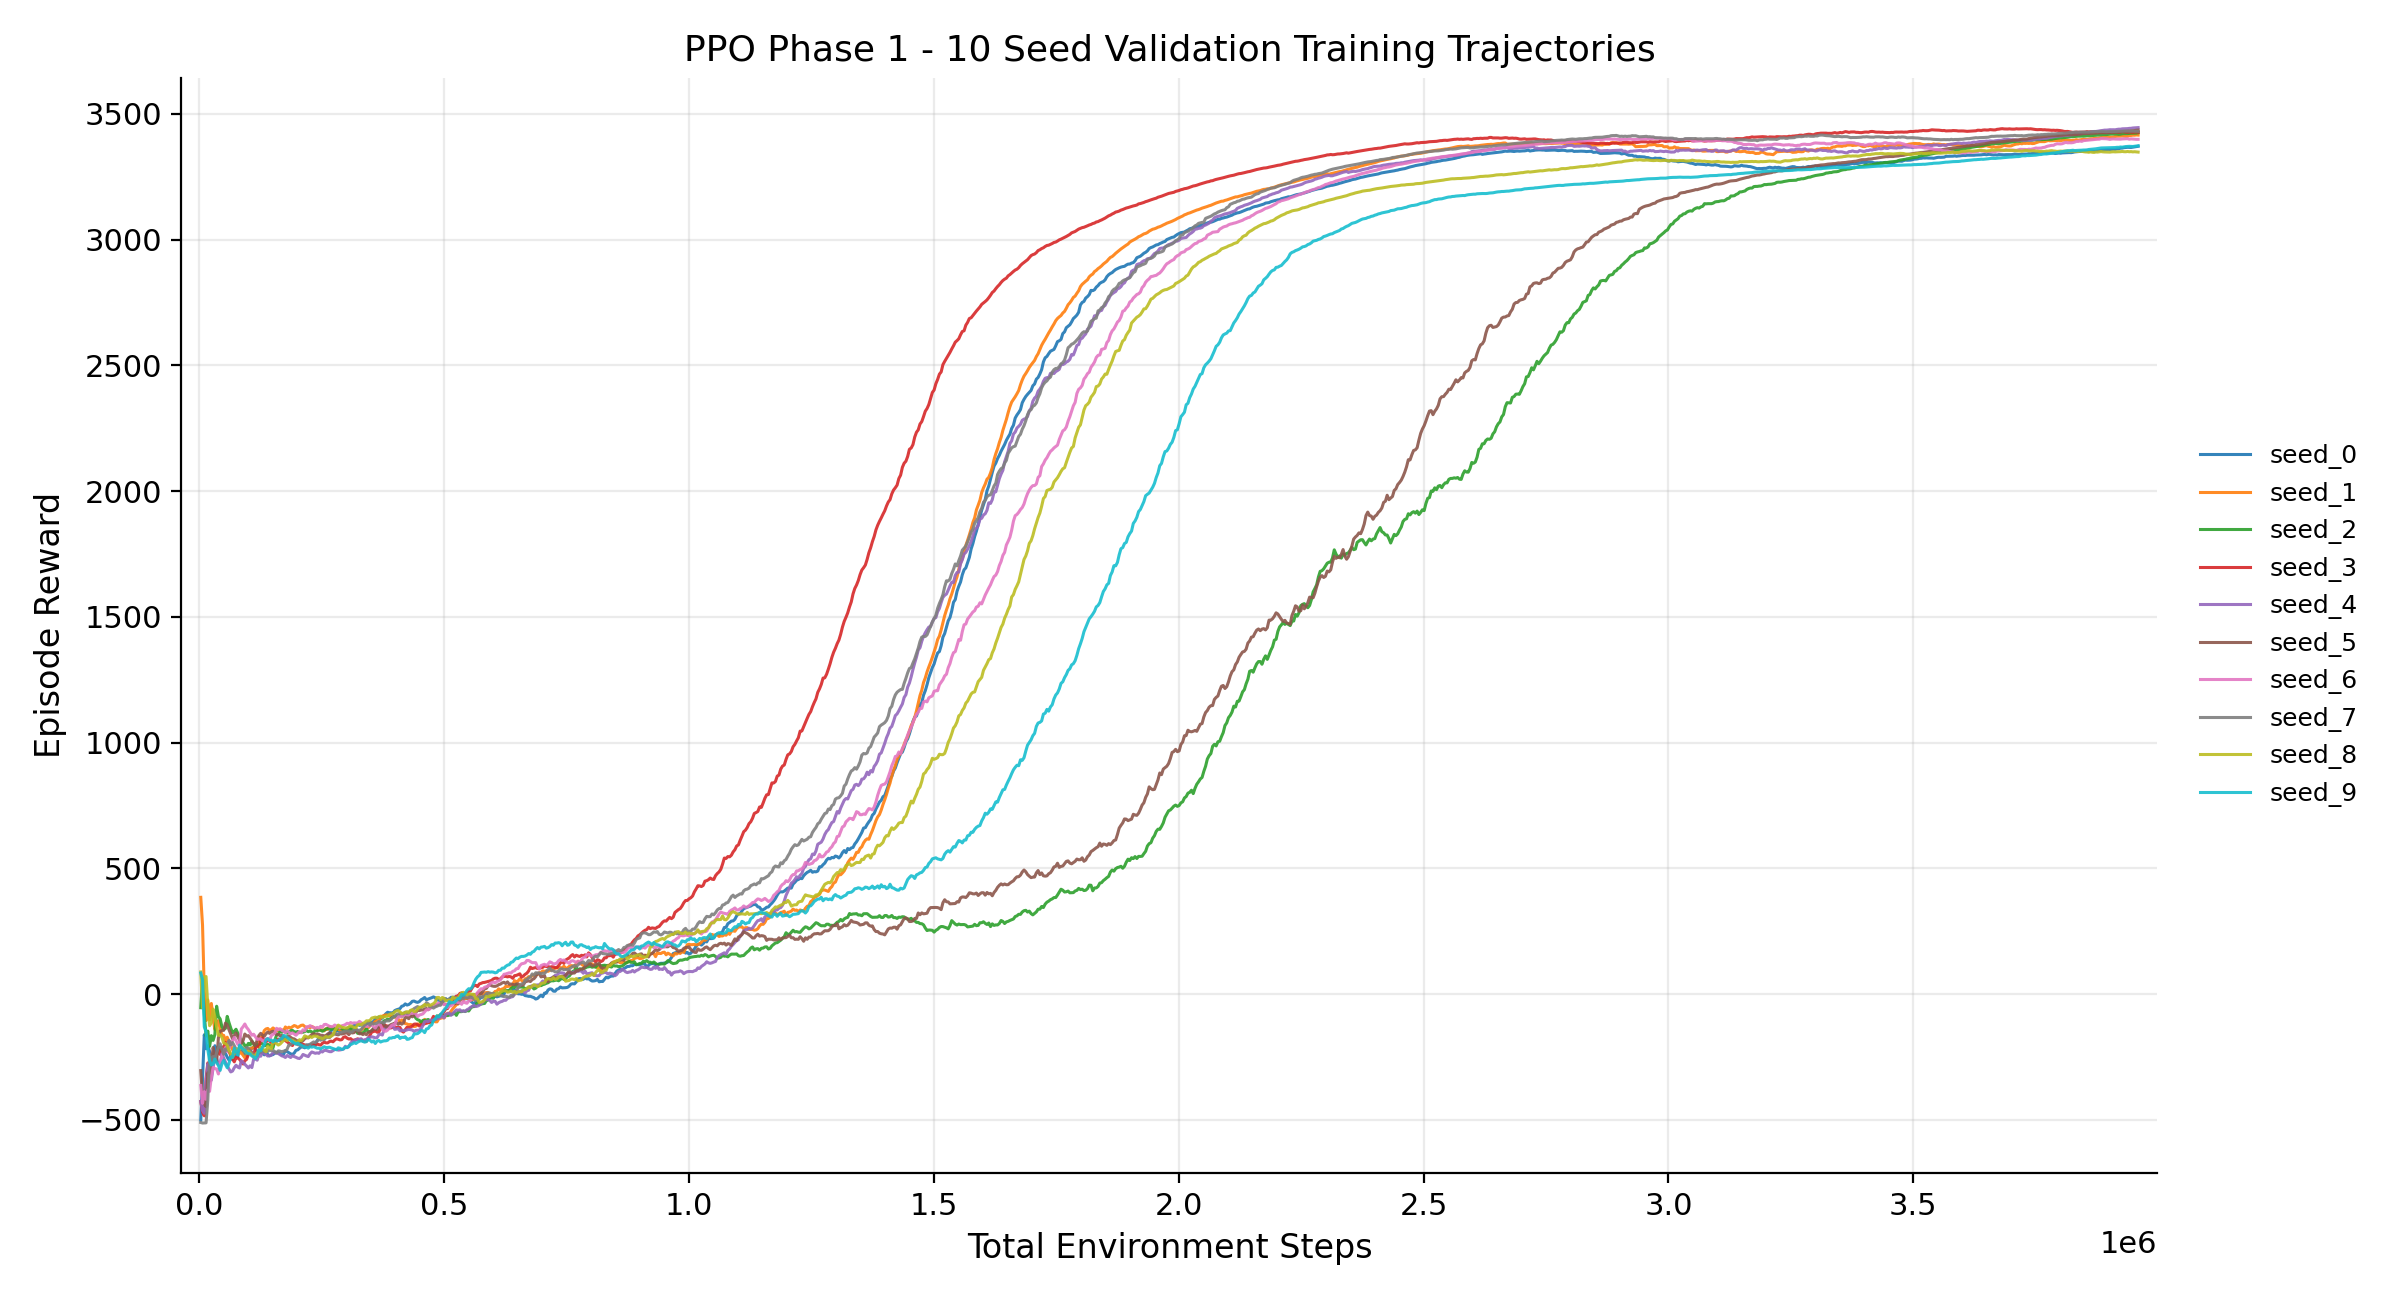
\includegraphics[width=0.75\textwidth]{imgs/plots/phase1/ppo/ppo_seeds.png}
  \caption[PPO seed training in Phase~1]{Training progress across different PPO seeds in Phase~1; curves are smoothed via moving average over 80 episodes.}
  \label{fig:phase1_ppo_seeds}
\end{figure}

\begin{figure}[htbp]
  \centering
  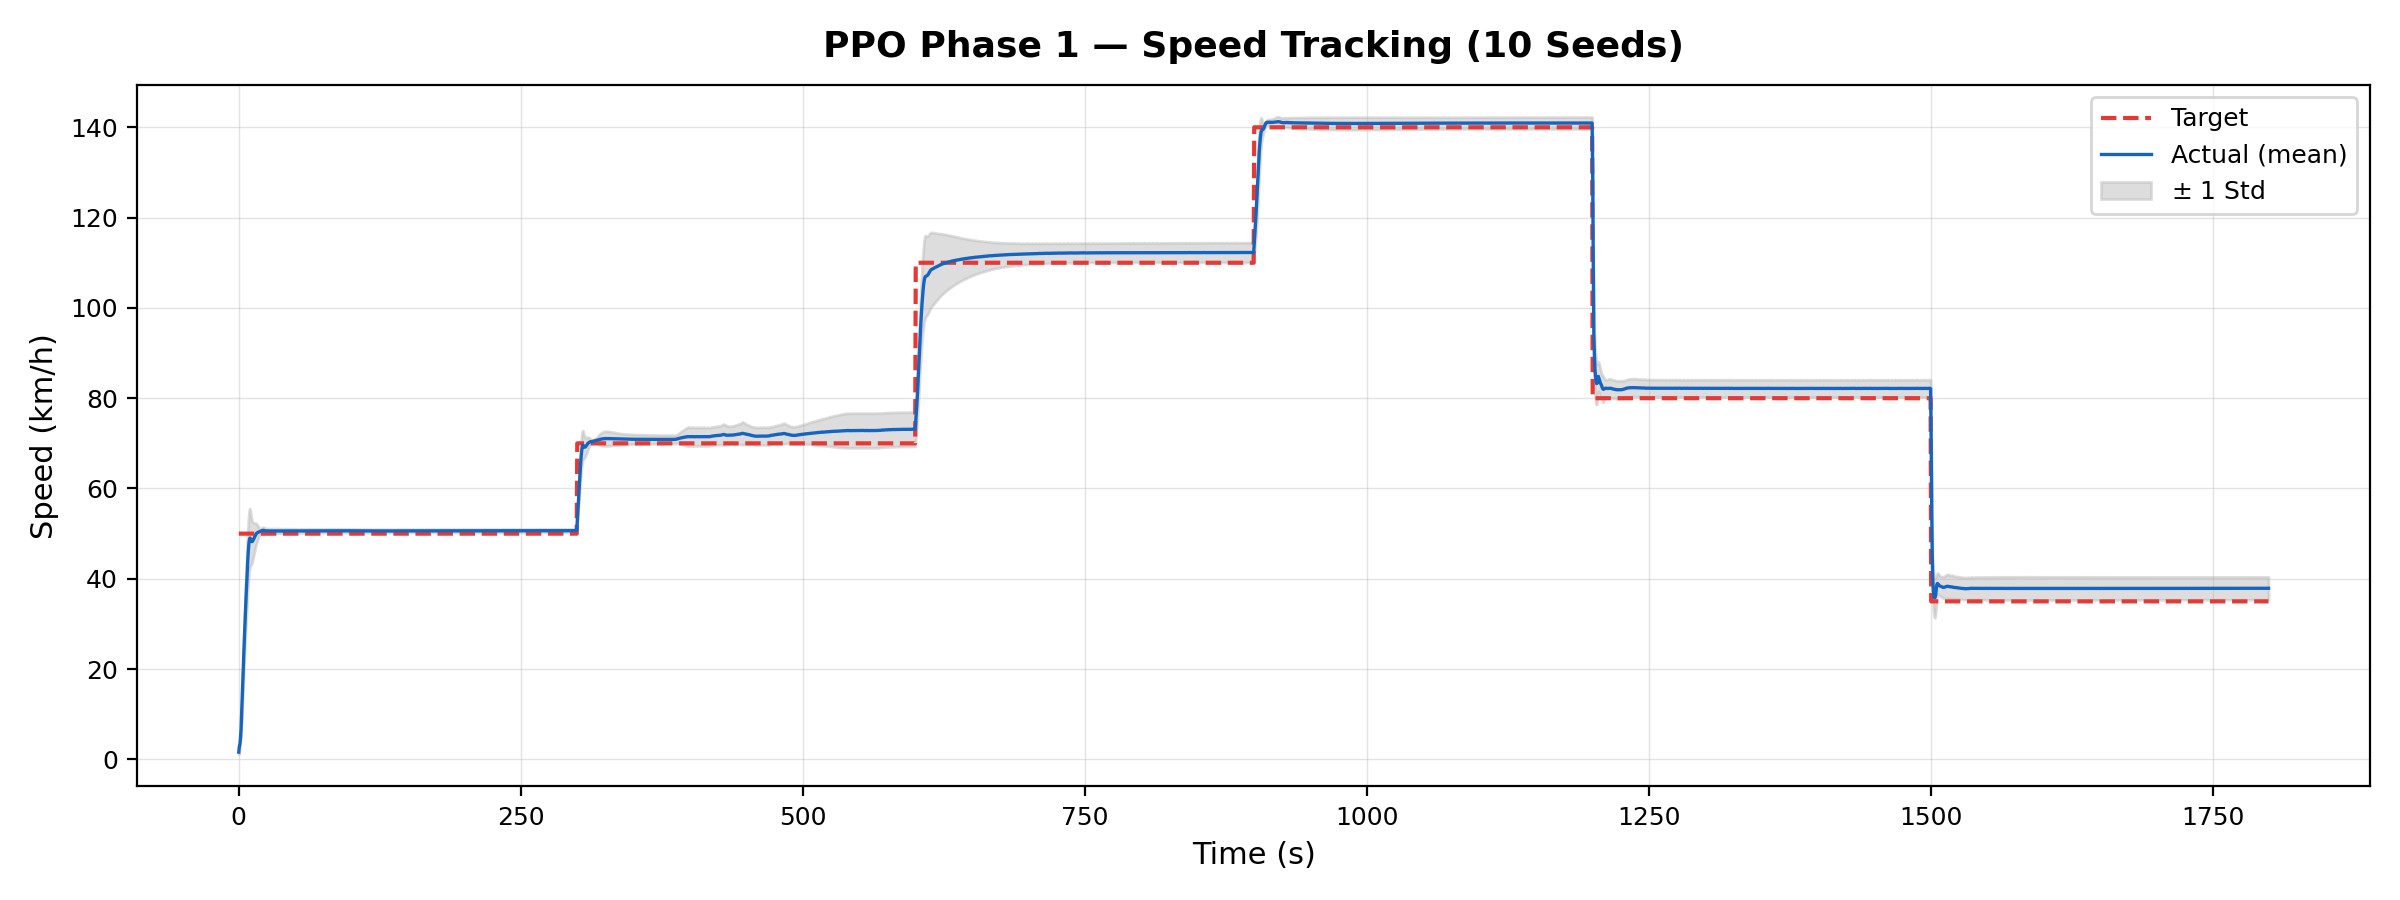
\includegraphics[width=0.7\textwidth]{imgs/plots/phase1/ppo/eval_speed_tracking.png}
  \caption[PPO speed tracking in Phase~1]{Evaluation speed-tracking trajectory for PPO in Phase~1.}
  \label{fig:phase1_ppo_eval_rmse_tracking}
\end{figure}

\paragraph{The best seed.}
The best PPO checkpoint is seed~3. Its action summary in \autoref{fig:phase1_ppo_action_summary} shows a high-rpm strategy. The engine is almost exclusively on, while the \ac{ICE} speed is concentrated at $4{,}000$\,rpm basically across the full target-speed range. The \ac{EM2} torque remains close to zero with only mild positive torque in the $0$--$80$\,Nm range, the fuel command is tightly concentrated around $17$--$23$\,mg, and the brake is essentially unused. This fixed operating point produces the cleanest best-seed policy of all three algorithms: $5.57$\,g cumulative \ac{NOx} and $74.46$\,g fuel at $3.16$\,km/h \ac{RMSE}. The result also shows that high engine speed alone is not the dominant \ac{NOx} driver; the integrated fuel seems more decisive. The resulting velocity, \ac{SOC}, and tailpipe \ac{NOx} emissions are depicted in \autoref{fig:phase1_ppo_seed3_evaluation_results}.

\begin{figure}[H]
  \centering
  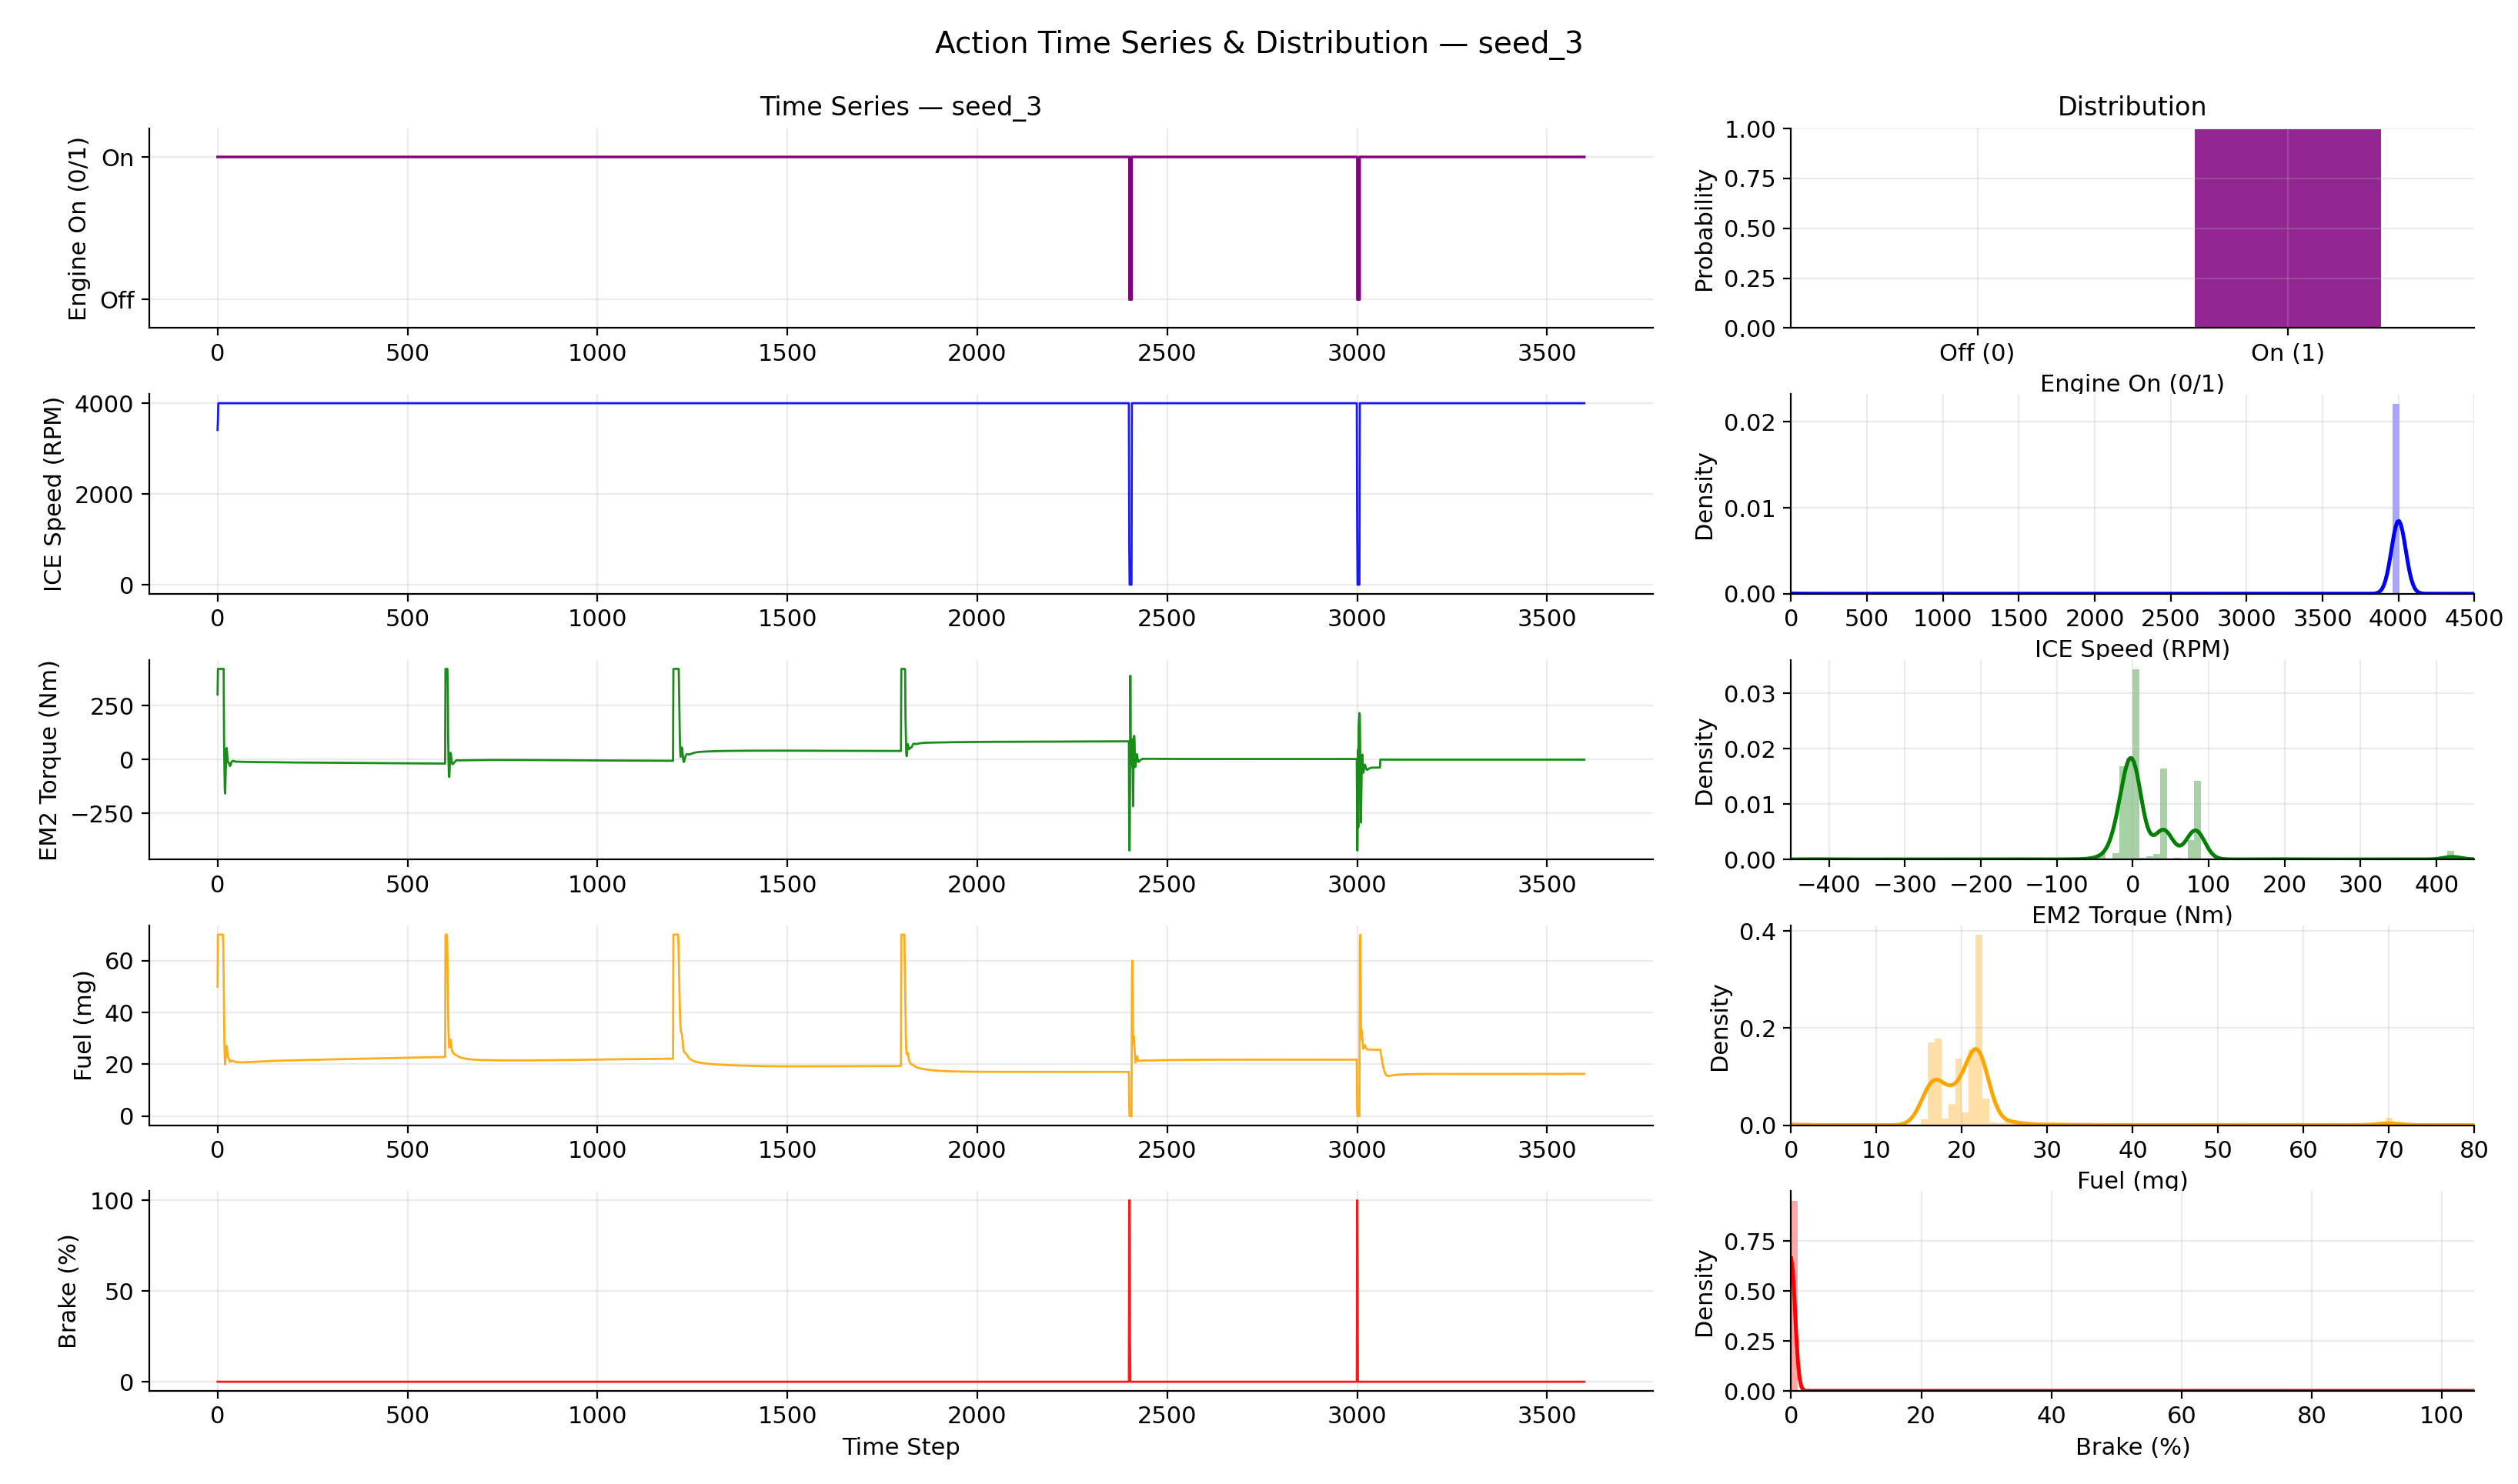
\includegraphics[width=\textwidth]{imgs/plots/phase1/ppo/seed_3_action_summary.png}
  \caption[Best PPO seed action summary in Phase~1]{Action summary for the best PPO checkpoint, seed~3, in Phase~1. The left panels show the PPO agent's actions during the evaluation cycle; the right panels show the corresponding densities.}
  \label{fig:phase1_ppo_action_summary}
\end{figure}

\begin{figure}[H]
  \centering
  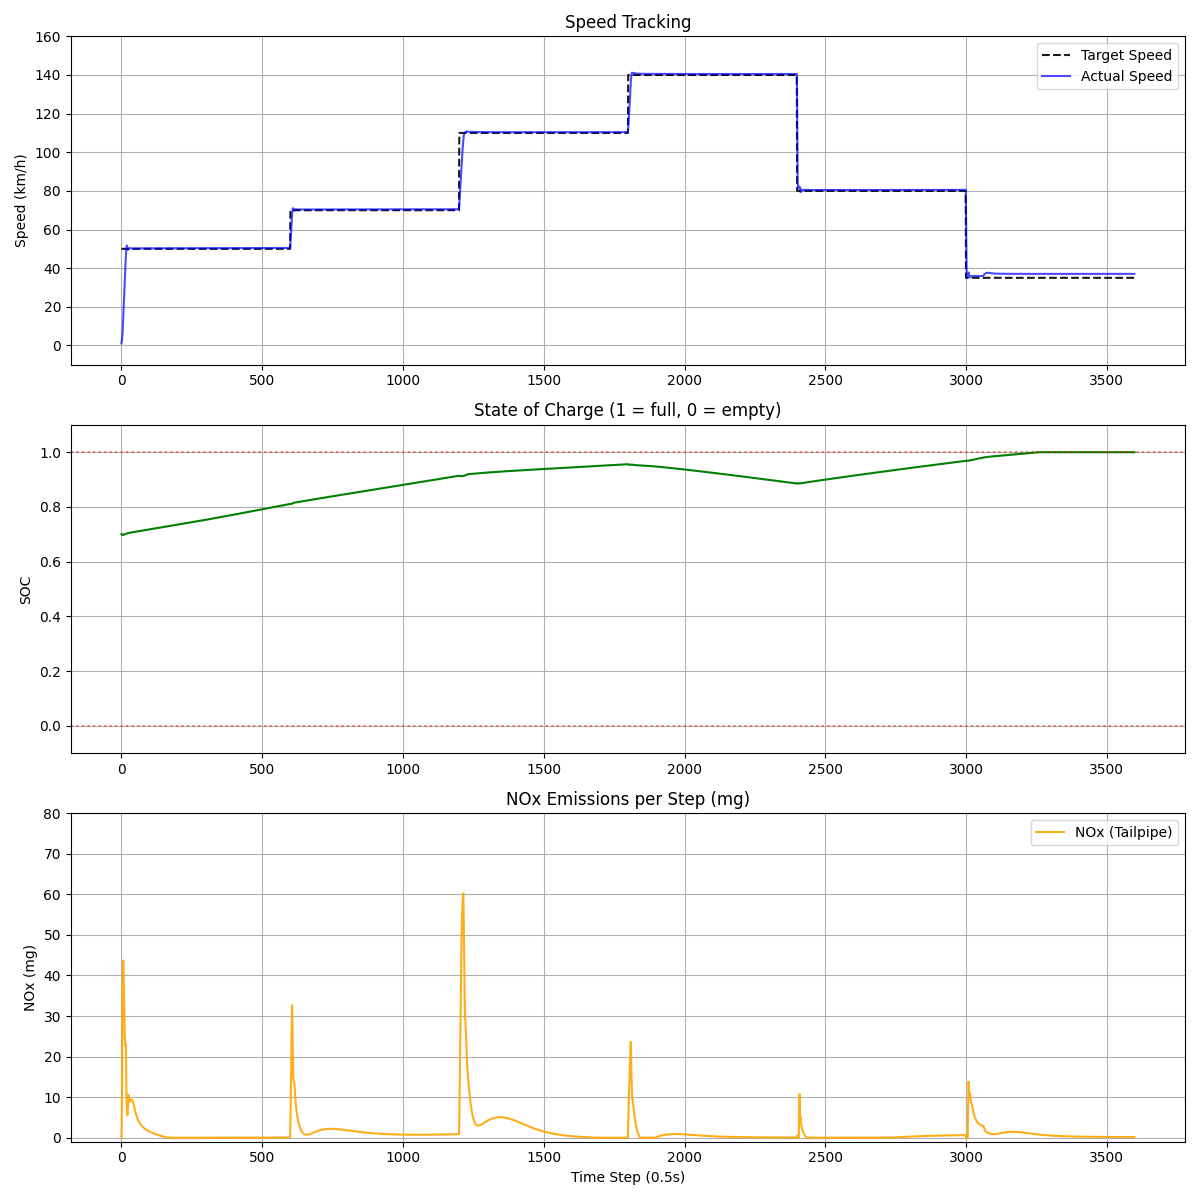
\includegraphics[width=0.55\textwidth]{imgs/plots/phase1/ppo/seed_3_evaluation_results.png}
  \caption[Best PPO seed evaluation results in Phase~1]{Evaluation results for the best PPO checkpoint, seed~3, in Phase~1. The panels show speed tracking, the \ac{SOC} trajectory, and tailpipe \ac{NOx} emissions over the evaluation cycle.}
  \label{fig:phase1_ppo_seed3_evaluation_results}
\end{figure}

\subsection{TD3}
\label{subsec:results_td3}
\paragraph{Hyperparameter optimisation trials.}

TD3's Optuna study comprised $45$ sampled trials, of which $30$ completed, $8$ were pruned, and the remaining $7$ failed; the corresponding trial history is shown in \autoref{fig:phase1_td3_trials}. The best configuration (\autoref{tab:phase1_best_hyperparameters} in Appendix~\ref{app:phase1_hyperparams}) features a learning rate of $1.79 \times 10^{-4}$, a batch size of $1{,}024$, a $[128, 128]$ \ac{MLP}, and most notably a \texttt{policy\_delay} of $1$. Setting the policy delay to $1$ effectively switches off the delayed actor-update mechanism that distinguishes \ac{TD3} from its predecessor \ac{DDPG}. The twin critics with clipped Gaussian target-policy smoothing ($\sigma_{\text{target}} = 0.116$, clip $= 0.7$) and the exploration noise ($\sigma_{\text{action}} = 0.144$) remain active. In this environment, the delayed actor update is therefore not what stabilises learning, an observation that is discussed further in \autoref{sec:findings_takeaways}.

\paragraph{Seed runs.}
The seed-wise learning curves (\autoref{fig:phase1_td3_seeds}) exhibit a fast initial climb to their plateau within the first $500{,}000$ steps. A single seed was not able to learn that fast initially and could only find a policy to cumulate the amount of reward at approximately $1{,}500{,}000$ steps. Different to \ac{PPO} however, is that the runs did not keep their stability once they reached the plateau. Instead, some of them drift off to a worse policy and then recover again or end with a slightly lower episode reward.

TD3 produces the tightest \ac{RMSE} distribution of the three algorithms ($3.81 \pm 0.29$\,km/h, \autoref{fig:phase1_td3_eval_rmse_tracking}) but at the same time the widest energy-side distribution ($95.4 \pm 100.8$\,g \ac{NOx}, $122.6 \pm 56.9$\,g fuel). The mean $\Delta\text{SOC}$ of $+0.146$ hides a bimodal underlying distribution: seeds $0$, $6$, and $8$ deplete the battery ($\Delta\text{SOC} = -0.12$, $-0.49$, $-0.03$ respectively), whereas the remaining seven seeds saturate it. Both groups can track the reference speed similarly well, which explains why the \ac{RMSE} distribution remains narrow while the energy- and emission-side distributions are much wider.

\begin{figure}[htbp]
  \centering
  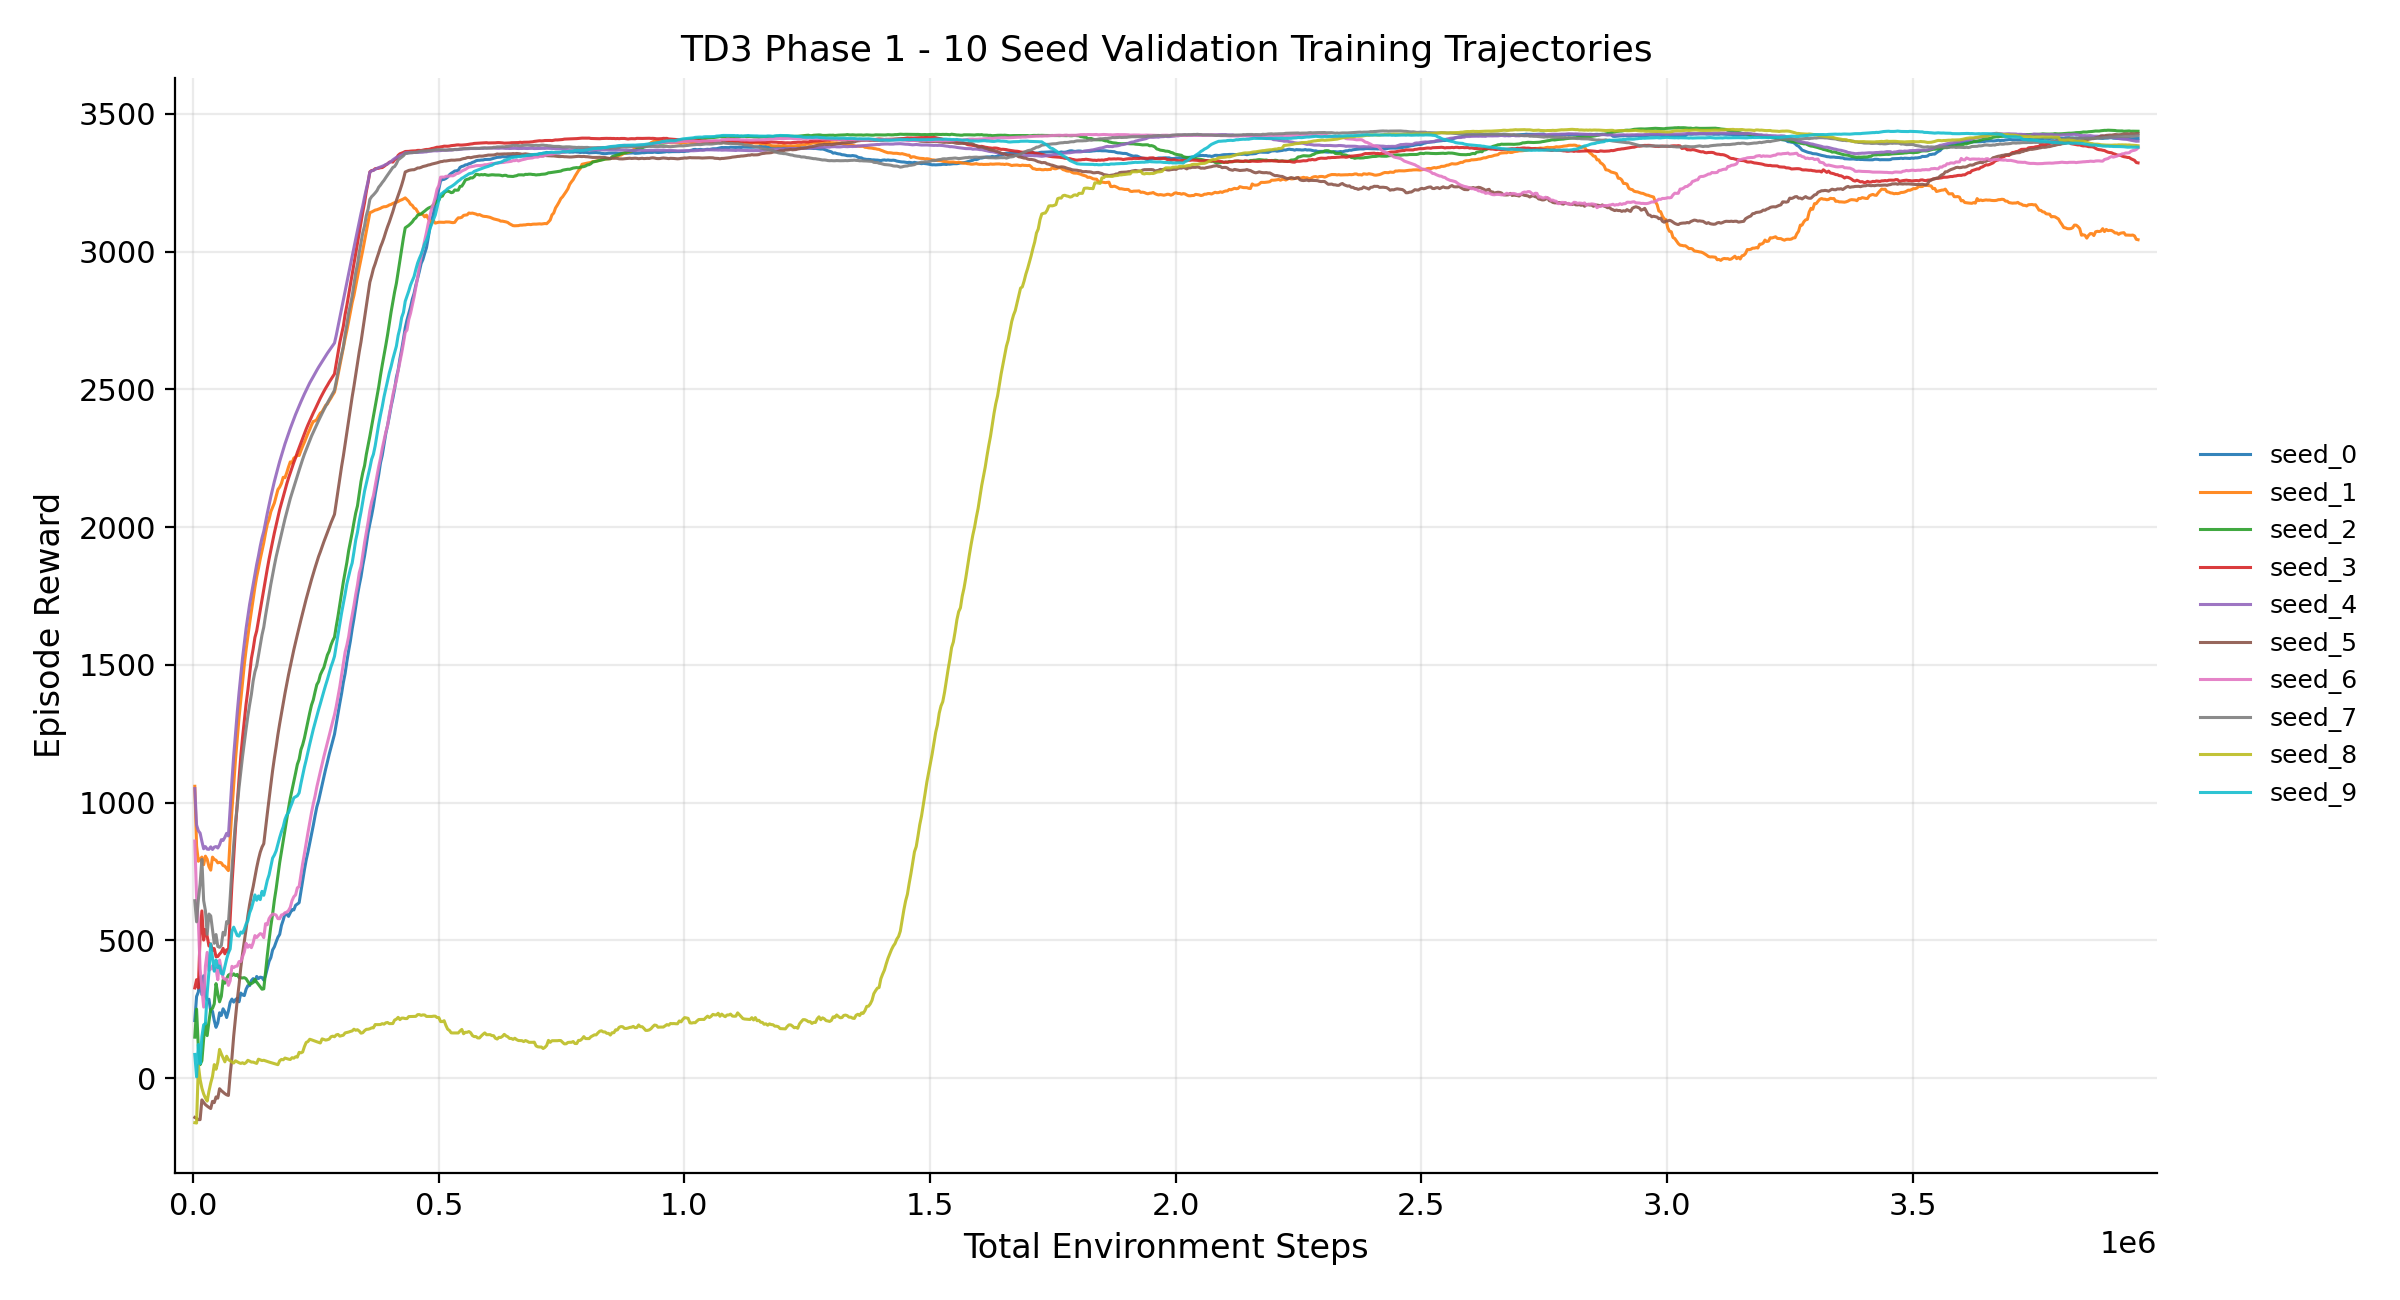
\includegraphics[width=0.75\textwidth]{imgs/plots/phase1/td3/td3_seeds.png}
  \caption[TD3 seed training in Phase~1]{Training progress across different TD3 seeds in Phase~1; curves are smoothed via moving average over 80 episodes.}
  \label{fig:phase1_td3_seeds}
\end{figure}

\begin{figure}[htbp]
  \centering
  
\includegraphics[width=0.7\textwidth]{imgs/plots/phase1/td3/eval_speed_tracking.png}
  \caption[TD3 speed tracking in Phase~1]{Evaluation speed-tracking trajectory for TD3 in Phase~1.}
  \label{fig:phase1_td3_eval_rmse_tracking}
\end{figure}

\paragraph{The best seed.}
The best TD3 checkpoint is seed~1. Its action summary in \autoref{fig:phase1_td3_action_summary} shows a lower-rpm policy than \ac{PPO}, combined with a bimodal fuel distribution and highly volatile \ac{EM2} usage. The engine is again almost exclusively on, while the \ac{ICE} speed is concentrated mainly around $900$--$1{,}300$\,rpm and $2{,}000$--$2{,}500$\,rpm. The $4{,}000$\,rpm region is used only when the target speed in the evaluation cycle increases. During steady cruising periods, where the target speed remains constant, the \ac{EM2} torque is approximately $0$\,Nm. In the first staircase segment (up to step $600$), it is exclusively negative at around $-165$\,Nm. In the fourth segment, at the highest target velocity of $140$\,km/h, the \ac{EM2} torque becomes highly volatile and alternates between approximately $+330$\,Nm and $-250$\,Nm every other time step (0.5\,s). Fuel injection is clearly bimodal, with one cluster around $10$--$20$\,mg and another around $50$--$70$\,mg. This high-fuel cluster gives TD3 the worst best-seed fuel and emission values: $163.94$\,g fuel and $73.42$\,g cumulative \ac{NOx} at $3.52$\,km/h \ac{RMSE}. The resulting velocity, \ac{SOC}, and tailpipe \ac{NOx} emissions are depicted in \autoref{fig:phase1_td3_seed1_evaluation_results}.

\begin{figure}[H]
  \centering
  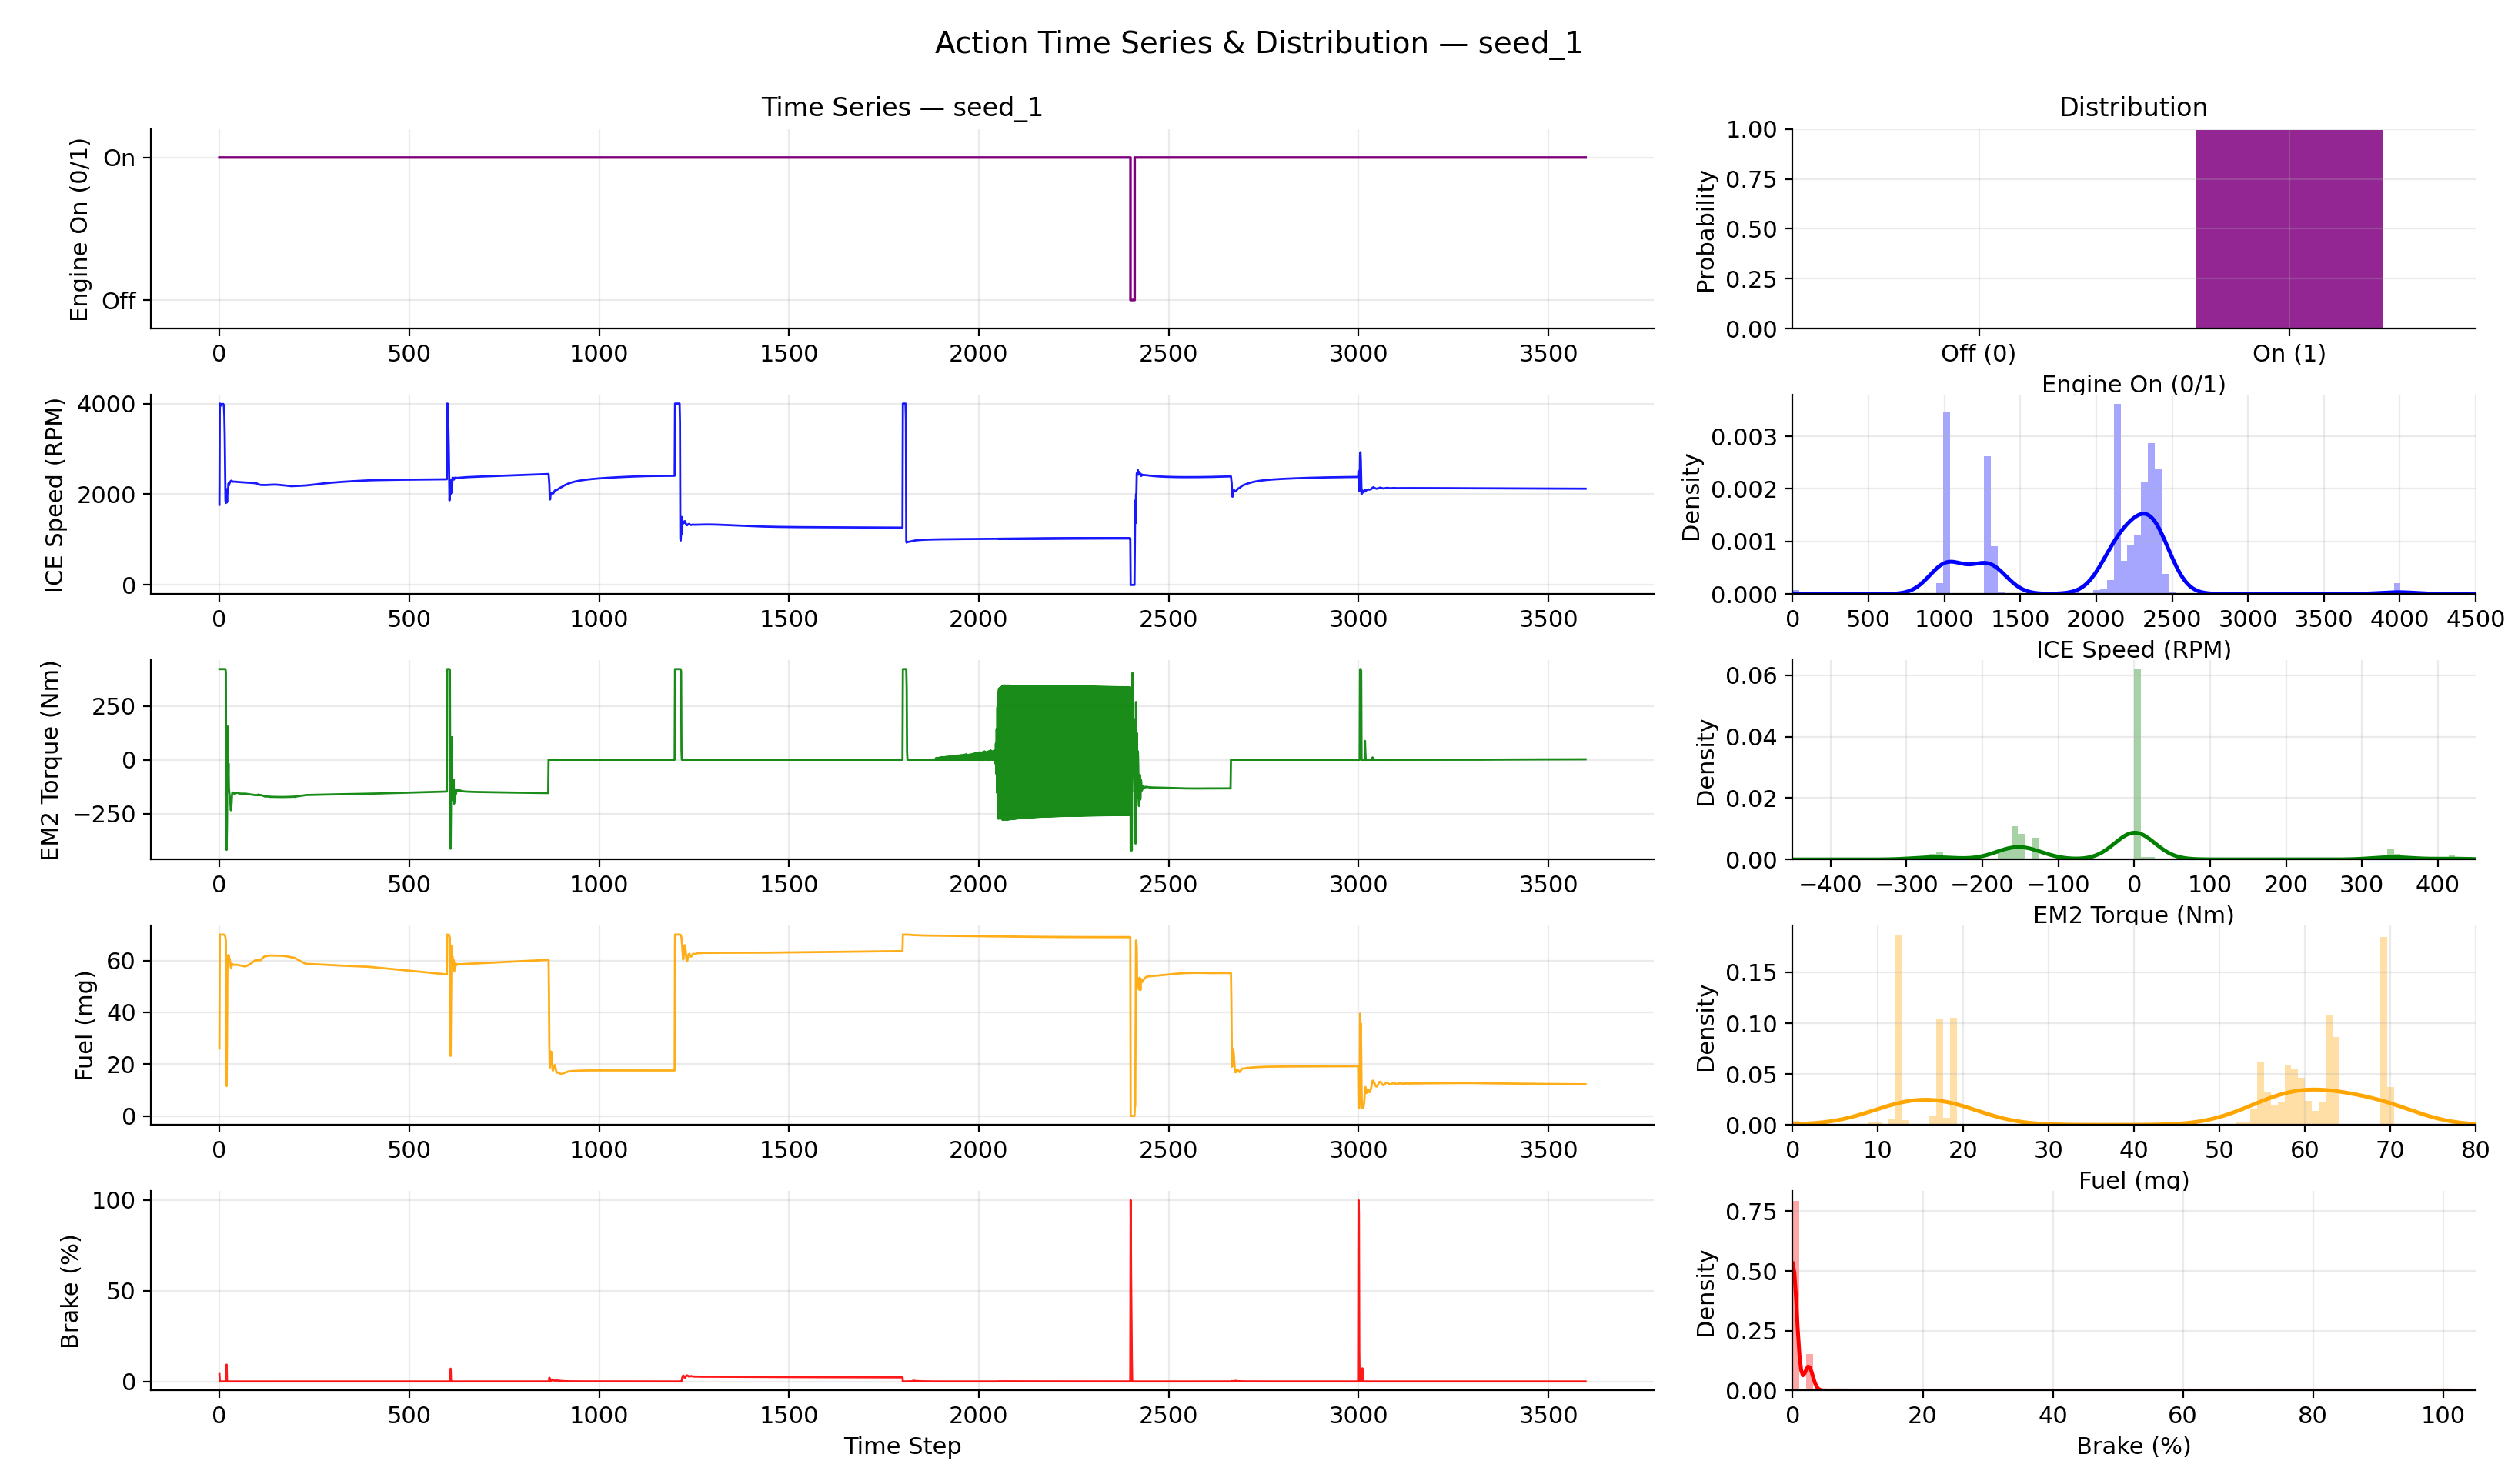
\includegraphics[width=\textwidth]{imgs/plots/phase1/td3/seed_1_action_summary.png}
  \caption[Best TD3 seed action summary in Phase~1]{Action summary for the best TD3 checkpoint, seed~1, in Phase~1. The left panels show the TD3 agent's actions during the evaluation cycle; the right panels show the corresponding densities.}
  \label{fig:phase1_td3_action_summary}
\end{figure}

\begin{figure}[H]
  \centering
  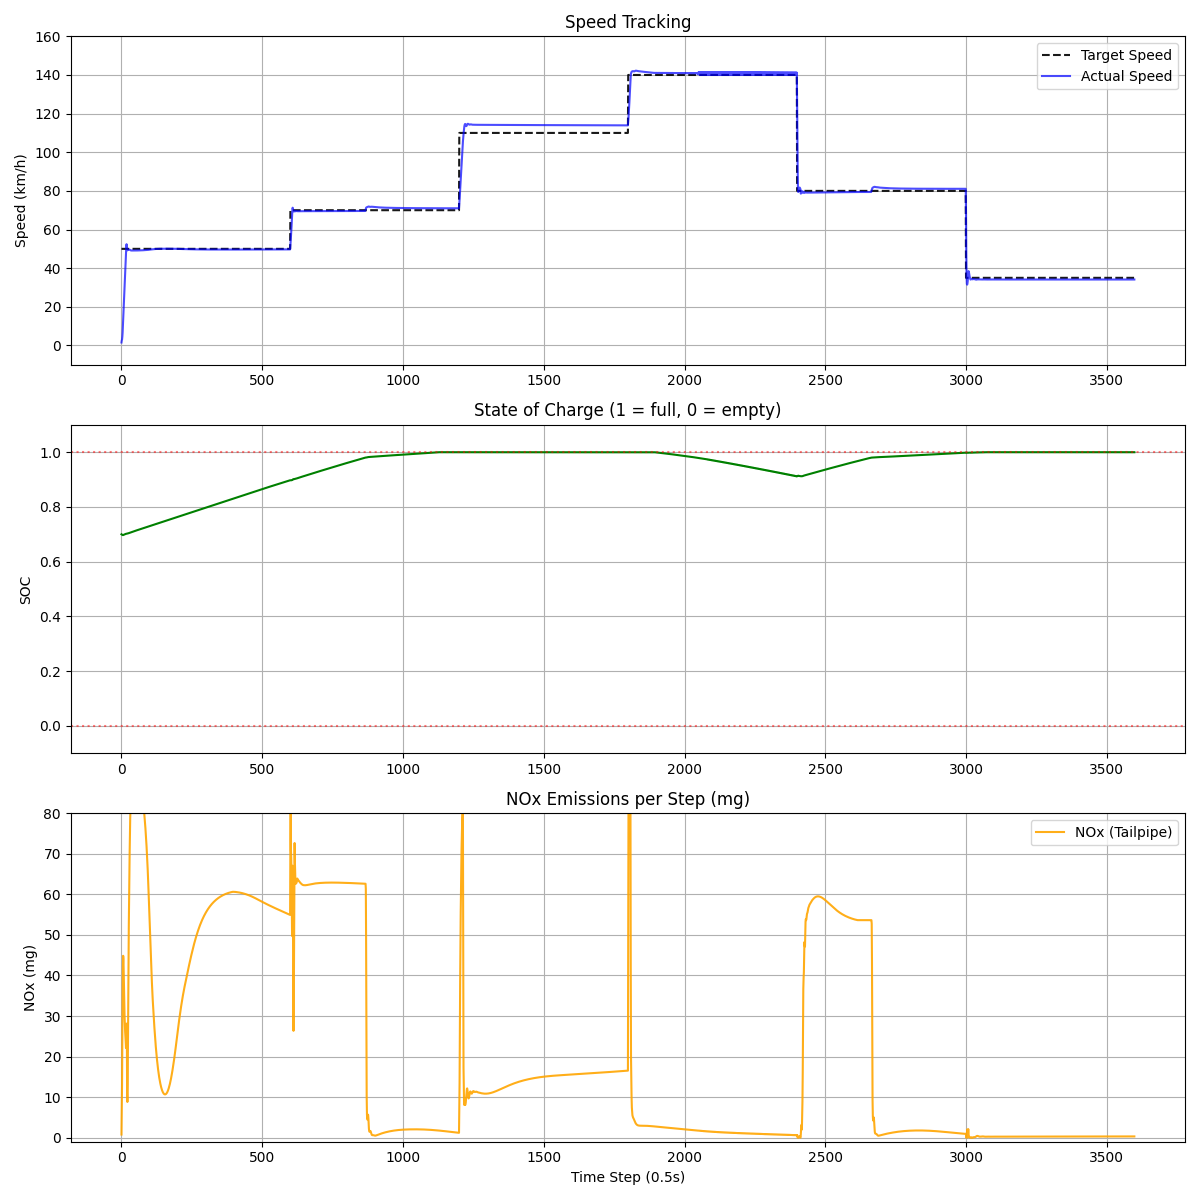
\includegraphics[width=0.55\textwidth]{imgs/plots/phase1/td3/seed_1_evaluation_results.png}
  \caption[Best TD3 seed evaluation results in Phase~1]{Evaluation results for the best TD3 checkpoint, seed~1, in Phase~1. The panels show speed tracking, the \ac{SOC} trajectory, and tailpipe \ac{NOx} emissions over the evaluation cycle.}
  \label{fig:phase1_td3_seed1_evaluation_results}
\end{figure}

\subsection{SAC}
\label{subsec:results_sac}

\paragraph{Hyperparameter optimisation trials.}
Of SAC's $44$ Optuna trials, $20$ completed successfully, $12$ were pruned, and $12$ failed; the corresponding trial history is shown in \autoref{fig:phase1_sac_trials}. The best configuration uses a learning rate of $9.20 \times 10^{-4}$, a batch size of $512$, a three-layer $[128, 128, 128]$ \ac{MLP}, $\tau = 0.0080$, and automatic entropy-coefficient tuning (\texttt{ent\_coef = "auto"}); the full configuration is documented in \autoref{tab:phase1_best_hyperparameters} in Appendix~\ref{app:phase1_hyperparams}.

\paragraph{Seed runs.}
The seed-wise learning curves (\autoref{fig:phase1_sac_seeds}) reach $\approx 3{,}500$ within $300{,}000$ steps and remain close to that level for the remainder of training, apart from two temporary dips around $3{,}300{,}000$ steps. SAC is more stable than TD3 because its reward trajectories are tighter, and it learns substantially faster than PPO; the two observed reward dips recover successfully and therefore do not indicate lasting instability. The resulting evaluation \ac{RMSE} ($3.45 \pm 0.43$\,km/h) has both the lowest mean and the lowest per-seed variance of the three algorithms (see \autoref{tab:phase1_summary}), making SAC the most reliable speed tracker in Phase~1.

\begin{figure}[htbp]
  \centering
  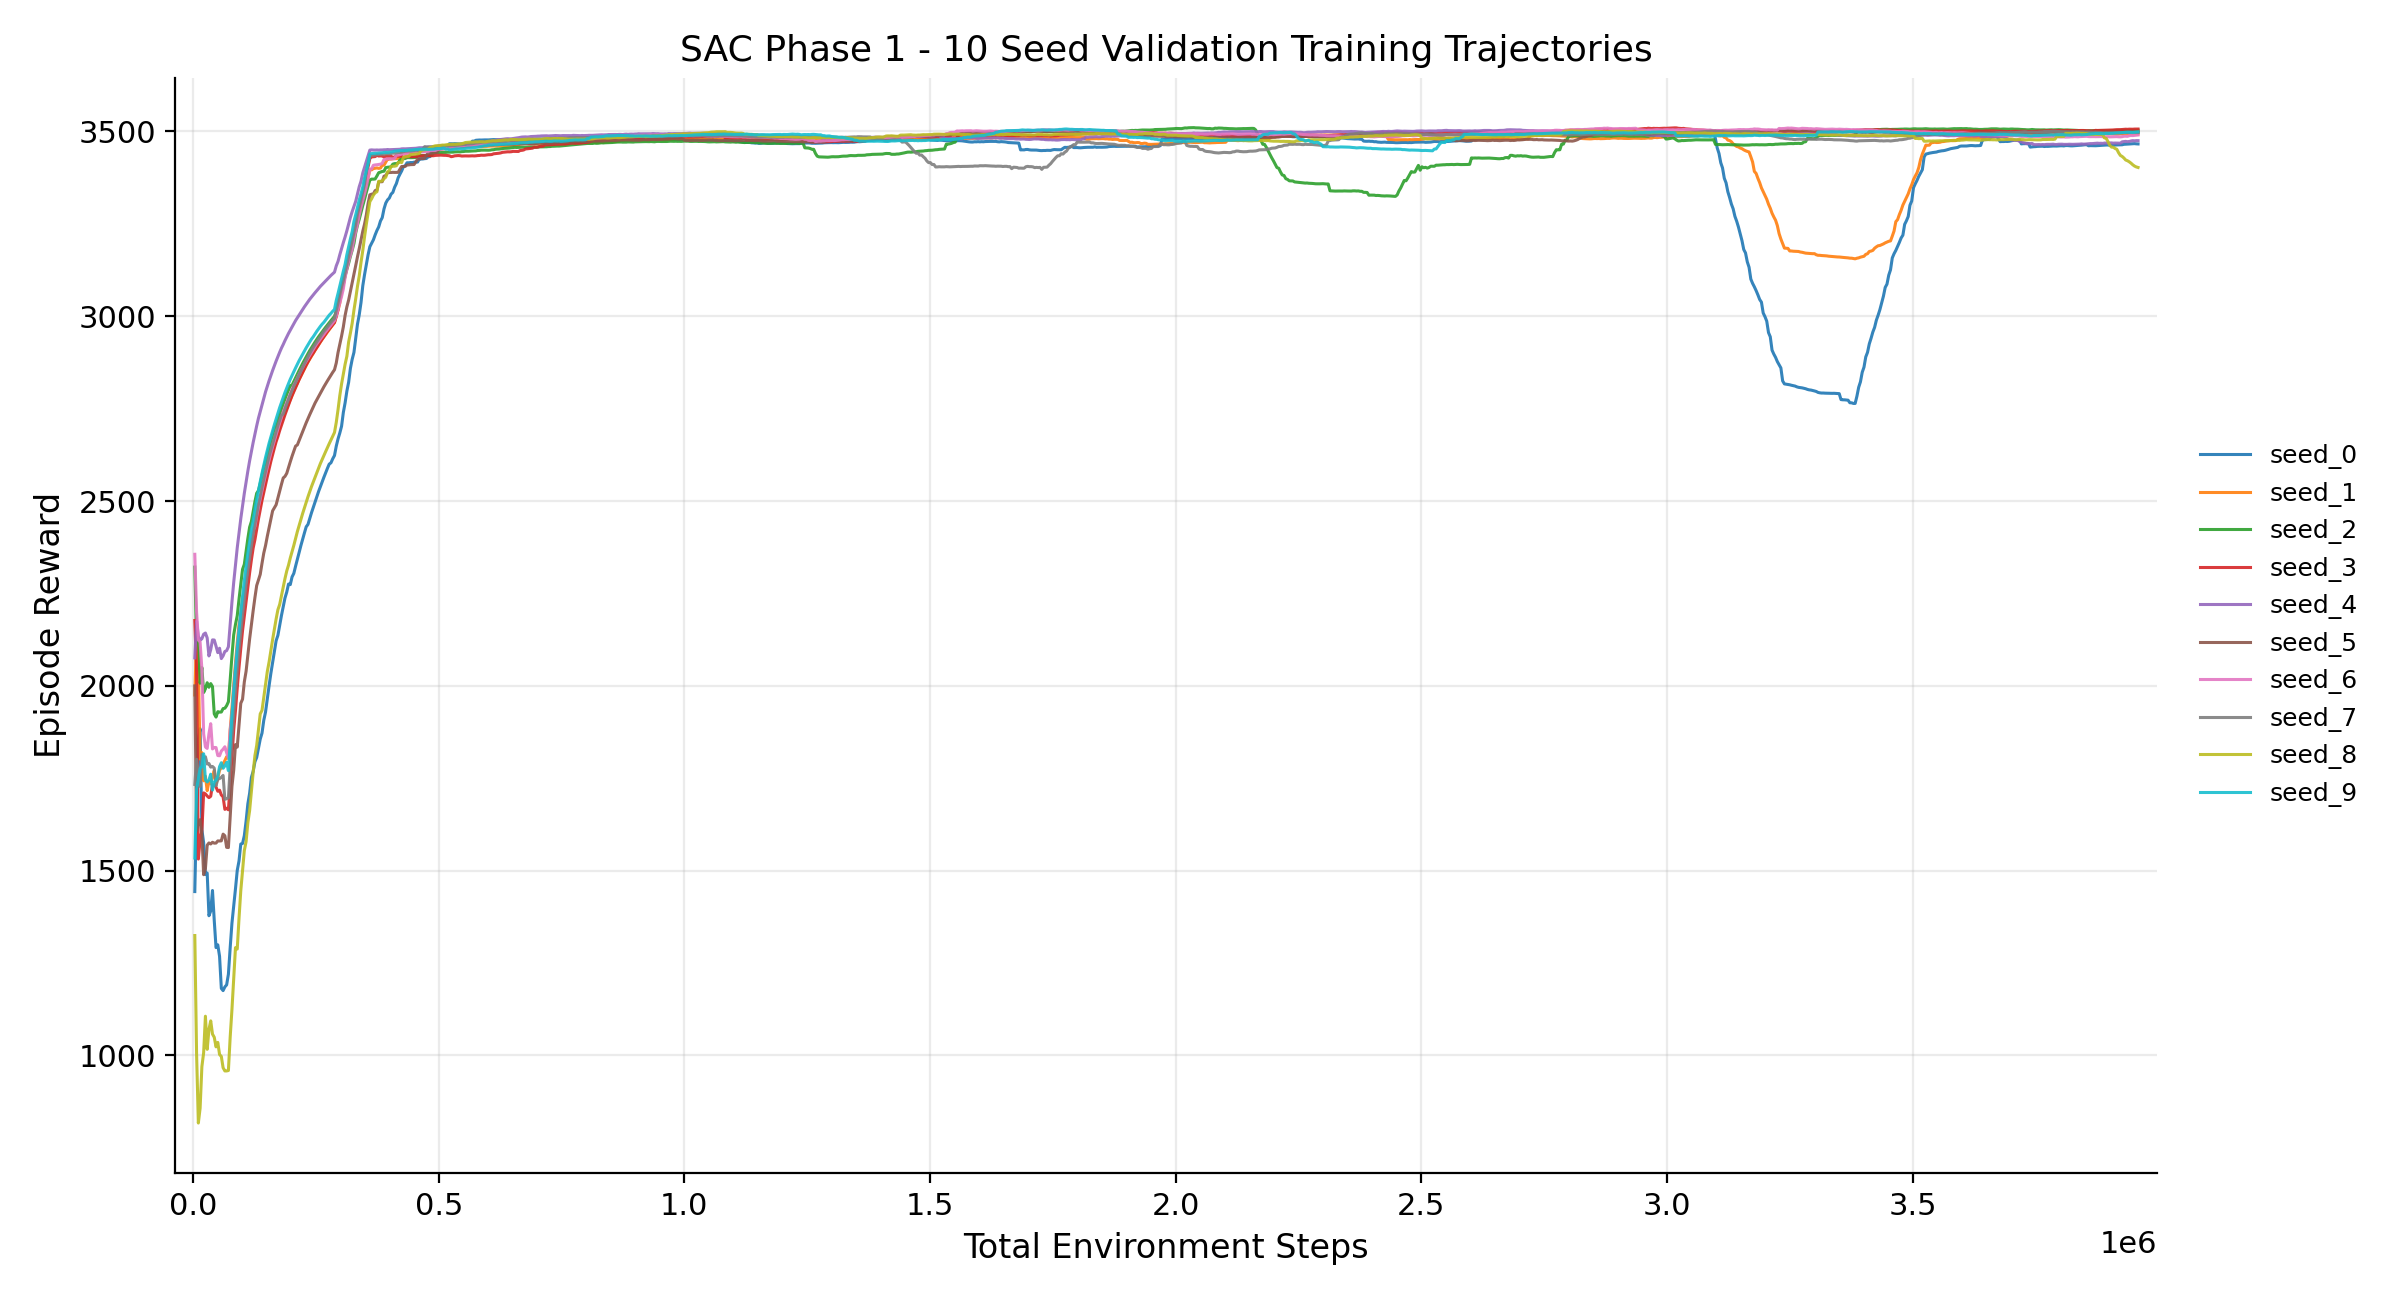
\includegraphics[width=0.75\textwidth]{imgs/plots/phase1/sac/sac_seeds.png}
  \caption[SAC seed training in Phase~1]{Training progress across different SAC seeds in Phase~1; curves are smoothed via moving average over 80 episodes.}
  \label{fig:phase1_sac_seeds}
\end{figure}

\begin{figure}[htbp]
  \centering
  
\includegraphics[width=0.7\textwidth]{imgs/plots/phase1/sac/eval_speed_tracking.png}
  \caption[SAC speed tracking in Phase~1]{Evaluation speed-tracking trajectory for SAC in Phase~1.}
  \label{fig:phase1_sac_eval_rmse_tracking}
\end{figure}

\paragraph{The best seed.}
The best SAC checkpoint is seed~3 and is also the lowest-\ac{RMSE} policy of Phase~1 across all algorithms. Its action summary in \autoref{fig:phase1_sac_action_summary} shows a more modulating strategy than PPO. The engine is active for most of the cycle, but it is switched off during the final staircase segment, making SAC the only best-seed policy that actively turns the engine off for a non-trivial part of the evaluation cycle. The \ac{ICE} speed therefore contains a $0$\,rpm mode and a broad active range from approximately $2{,}400$ to $4{,}000$\,rpm. The \ac{EM2} torque is mostly close to zero, with a negative presence at around $-50$ to $-100$\,Nm and a smaller positive band between $0$ and approximately $+70$\,Nm. In the engine-off segment, the agent alternates between these positive torque values every other step to propel the vehicle while the \ac{ICE} is off. Fuel injection is zero when the engine is off, due to the engine-switch cooldown through the post-posed action shield described in \autoref{sec:impl_environment}; otherwise, it is concentrated around $30$--$40$\,mg up to $60$\,mg. This learned behaviour yields the best speed tracking ($3.11$\,km/h \ac{RMSE} and $0.89$\,km/h \ac{MAE}), but it comes at higher cumulative fuel ($109.31$\,g) and \ac{NOx} ($48.94$\,g) than the best PPO seed. The resulting velocity, \ac{SOC}, and tailpipe \ac{NOx} emissions are depicted in \autoref{fig:phase1_sac_seed3_evaluation_results}.

\begin{figure}[H]
  \centering
  
\includegraphics[width=\textwidth]{imgs/plots/phase1/sac/seed_3_action_summary.png}
  \caption[Best SAC seed action summary in Phase~1]{Action summary for the best SAC checkpoint, seed~3, in Phase~1. The left panels show the SAC agent's actions during the evaluation cycle; the right panels show the corresponding densities.}
  \label{fig:phase1_sac_action_summary}
\end{figure}

\begin{figure}[H]
  \centering
  
\includegraphics[width=0.55\textwidth]{imgs/plots/phase1/sac/seed_3_evaluation_results.png}
  \caption[Best SAC seed evaluation results in Phase~1]{Evaluation results for the best SAC checkpoint, seed~3, in Phase~1. The panels show speed tracking, the \ac{SOC} trajectory, and tailpipe \ac{NOx} emissions over the evaluation cycle.}
  \label{fig:phase1_sac_seed3_evaluation_results}
\end{figure}

\subsection{Summary}
\label{subsec:results_phase1_summary}

\paragraph{Training convergence.}
The three algorithms reach essentially indistinguishable best-seed speed-tracking quality: the minimum-\ac{RMSE} seeds of PPO, SAC and TD3 fall within $3.11$--$3.51$\,km/h. The remaining error is dominated by the unavoidable transient overshoot at each step change in the staircase evaluation cycle, while the steady-state tracking on each plateau is much tighter. \autoref{fig:phase1_training_progress_comparison} also shows the typical sample-efficiency difference between the algorithms: SAC and TD3 reach their reward plateau earlier than PPO, whereas PPO converges more slowly under the same environment-interaction budget. By the end of training, however, all three algorithms operate close to the theoretical reward ceiling, so the central Phase~1 finding is not whether speed tracking can be learned, but which uncontrolled side effects appear once only speed tracking is rewarded.

\begin{figure}[H]
  \centering
  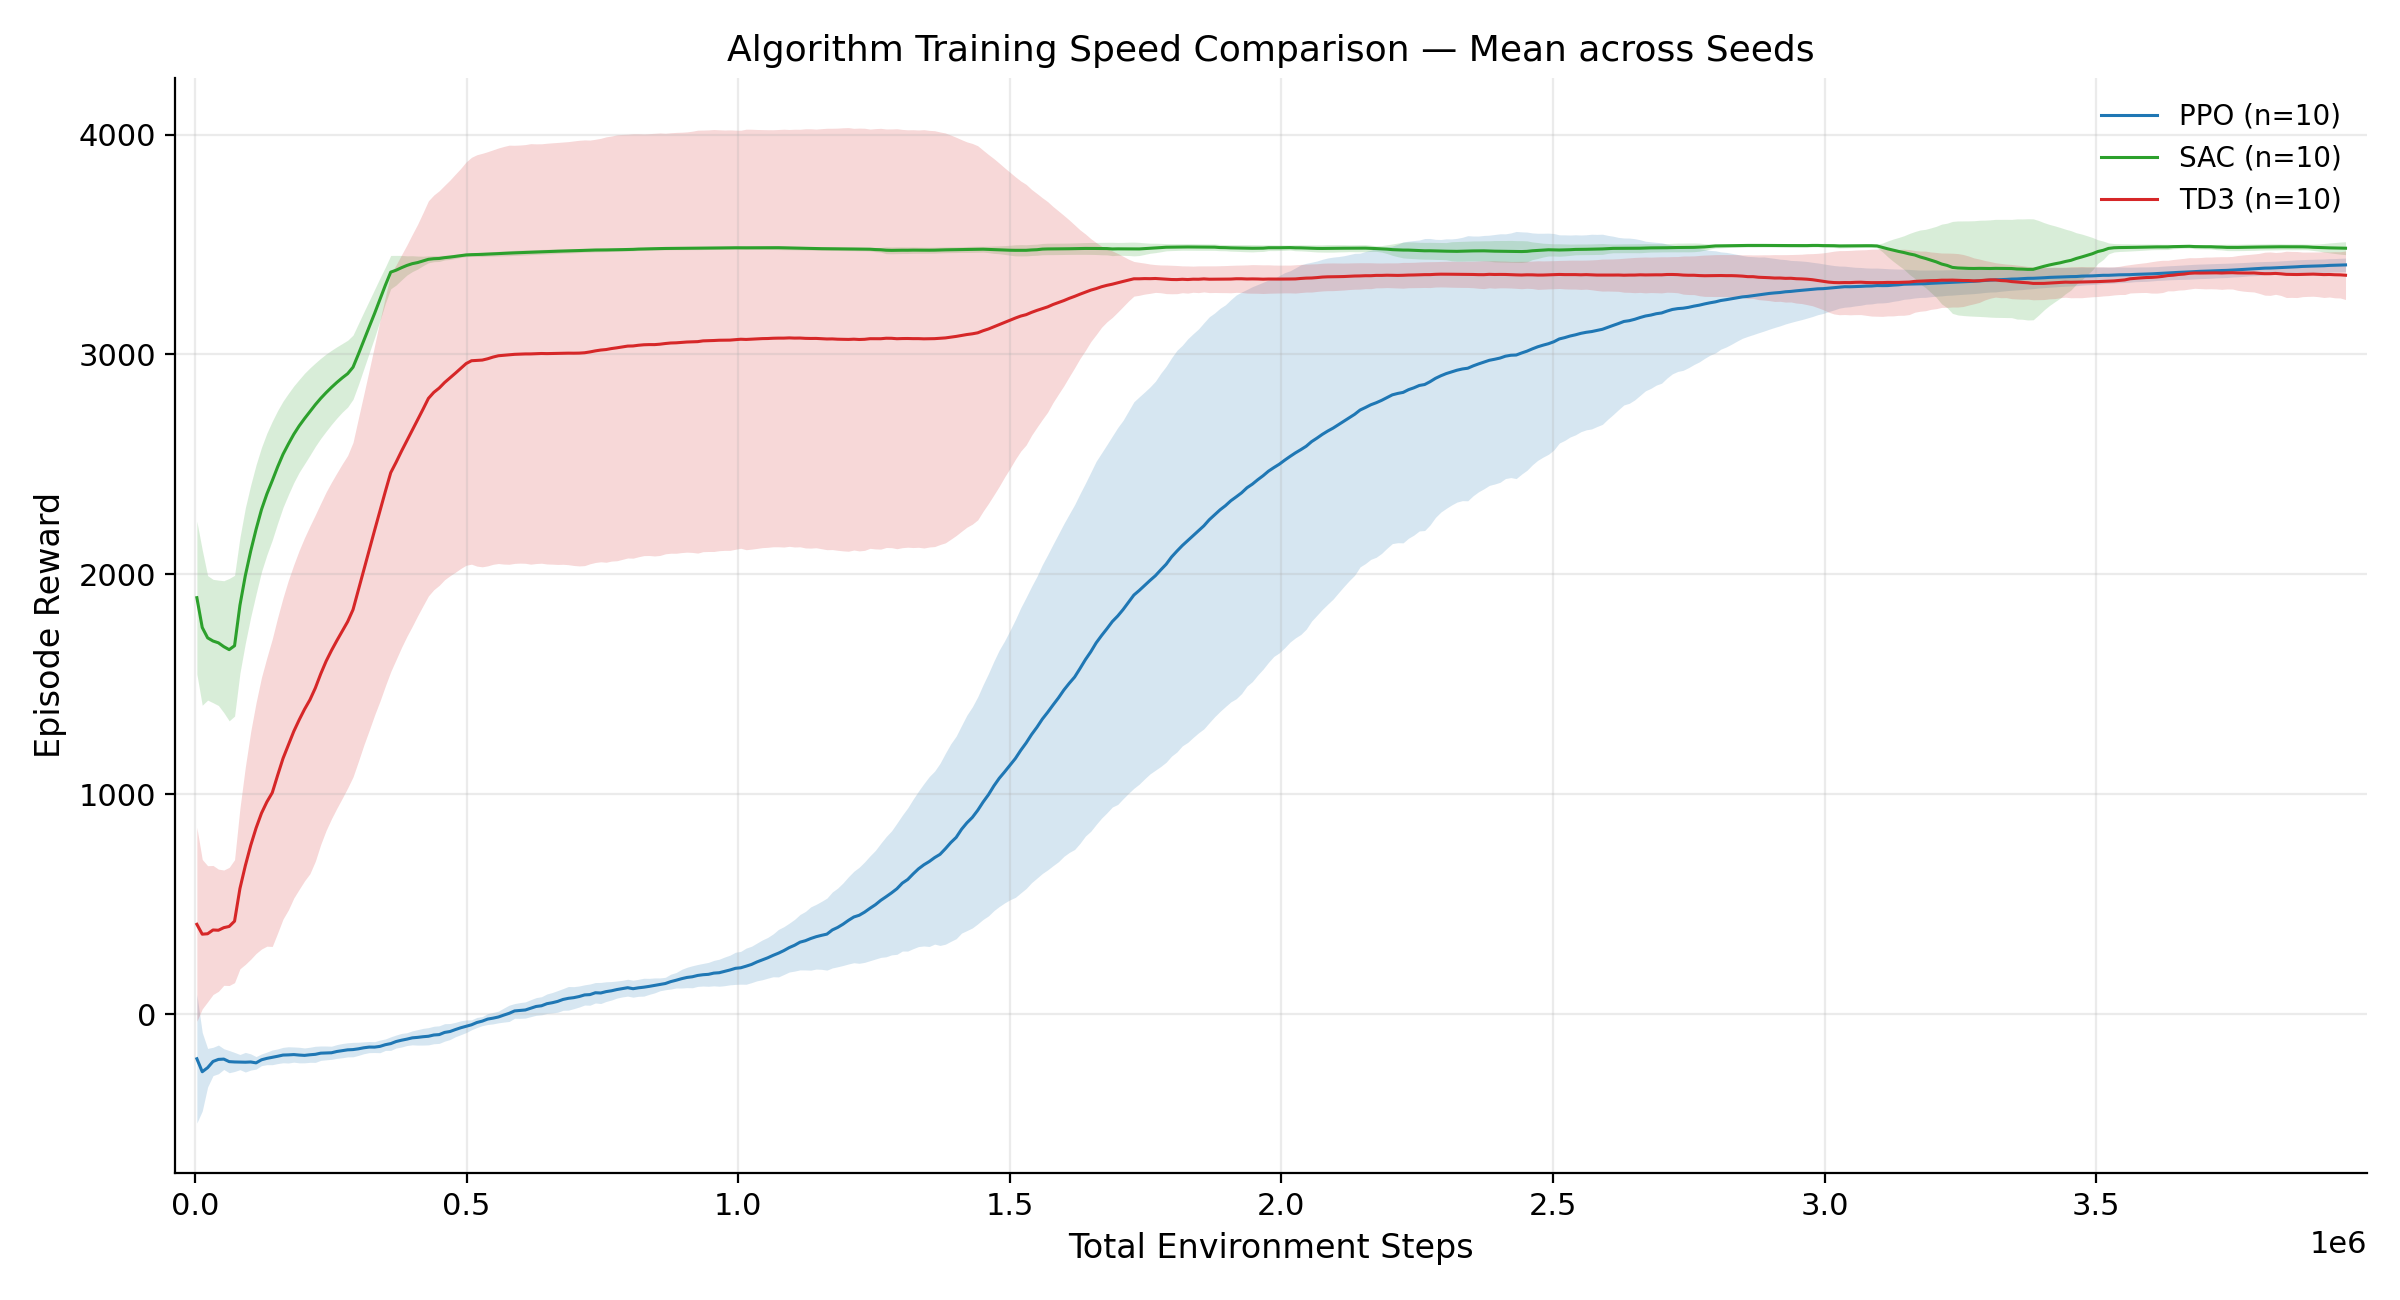
\includegraphics[width=0.7\textwidth]{imgs/plots/phase1/training_progress_comparison.png}
  \caption[Phase~1 training-progress comparison]{Comparison of seed-averaged training progress across all Phase~1 algorithms. Curves are smoothed with a moving average over 80 episodes, and shaded bands represent $\pm$ one standard deviation across the 10 seed curves at each x-grid point.}
  \label{fig:phase1_training_progress_comparison}
\end{figure}

\paragraph{Equal tracking but divergent powertrain use.}
To look behind the seed-averaged tracking quality, three cross-algorithm visualisations (\autoref{fig:phase1_pareto_front}--\autoref{fig:phase1_engine_map_occupancy}) dissect how the $30$ policies differ despite near-identical reward. The Pareto view in \autoref{fig:phase1_pareto_front} plots speed-tracking accuracy against cumulative \ac{NOx}. Speed tracking is tightly clustered (\ac{RMSE} $3.1$--$6.3$\,km/h), whereas cumulative \ac{NOx} spans more than two orders of magnitude ($2.6$--$354$\,g). The non-dominated low-\ac{NOx} front is occupied almost exclusively by battery-depleting policies --- for example SAC seed~8 attains only $2.6$\,g \ac{NOx} but at $\Delta\text{SOC}=-0.64$ --- while the majority of seeds saturate the battery upward ($\Delta\text{SOC}\approx+0.30$) and form a distinctly higher-\ac{NOx} band. The parallel-coordinate view in \autoref{fig:phase1_parallel_coords} confirms the same degeneracy across every metric at once: reward, \ac{RMSE} and \ac{MAE} stay nearly flat from seed to seed, whereas fuel, \ac{NOx} and $\Delta$\ac{SOC} fan out strongly. Equal speed-tracking reward therefore masks fundamentally different energy-management strategies, and a low \ac{NOx} value in Phase~1 is frequently the by-product of draining the unconstrained battery rather than of a charge-sustaining clean-control policy. This degeneracy is the direct motivation for the explicit \ac{SOC} and \ac{NOx} reward terms introduced in Phase~2.

\begin{figure}[htbp]
  \centering
  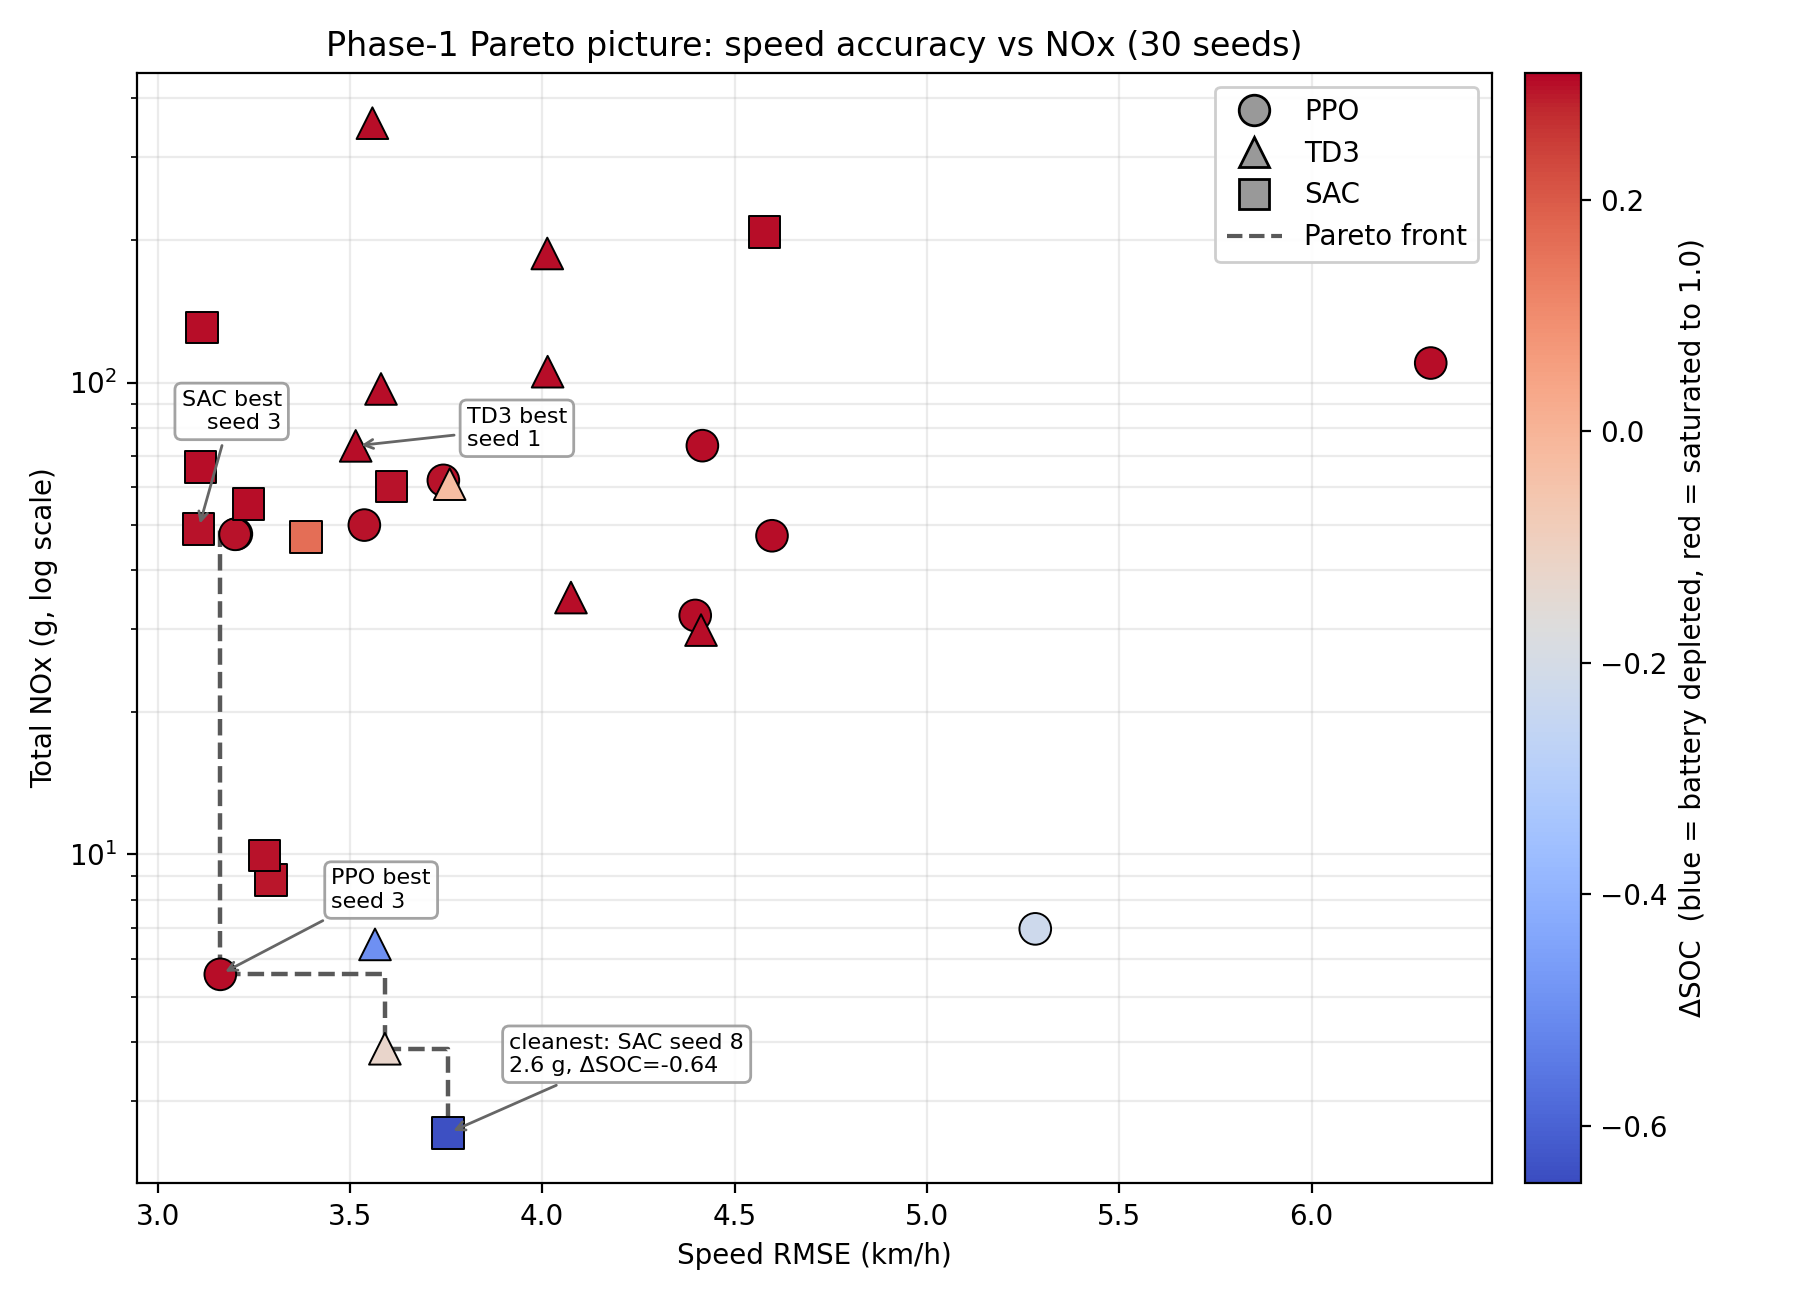
\includegraphics[width=0.7\textwidth]{imgs/analysis_plots/pareto_front.png}
  \caption[Speed-tracking accuracy versus NOx across all Phase~1 seeds]{Speed-tracking accuracy versus \ac{NOx} across all 30 Phase~1 seeds on the deterministic staircase evaluation cycle. Marker shape encodes the algorithm, fill colour encodes the net battery-state change $\Delta$\ac{SOC}, and the dashed step line denotes the non-dominated front for jointly minimising \ac{RMSE} and \ac{NOx}.}
  \label{fig:phase1_pareto_front}
\end{figure}

\begin{figure}[htbp]
  \centering
  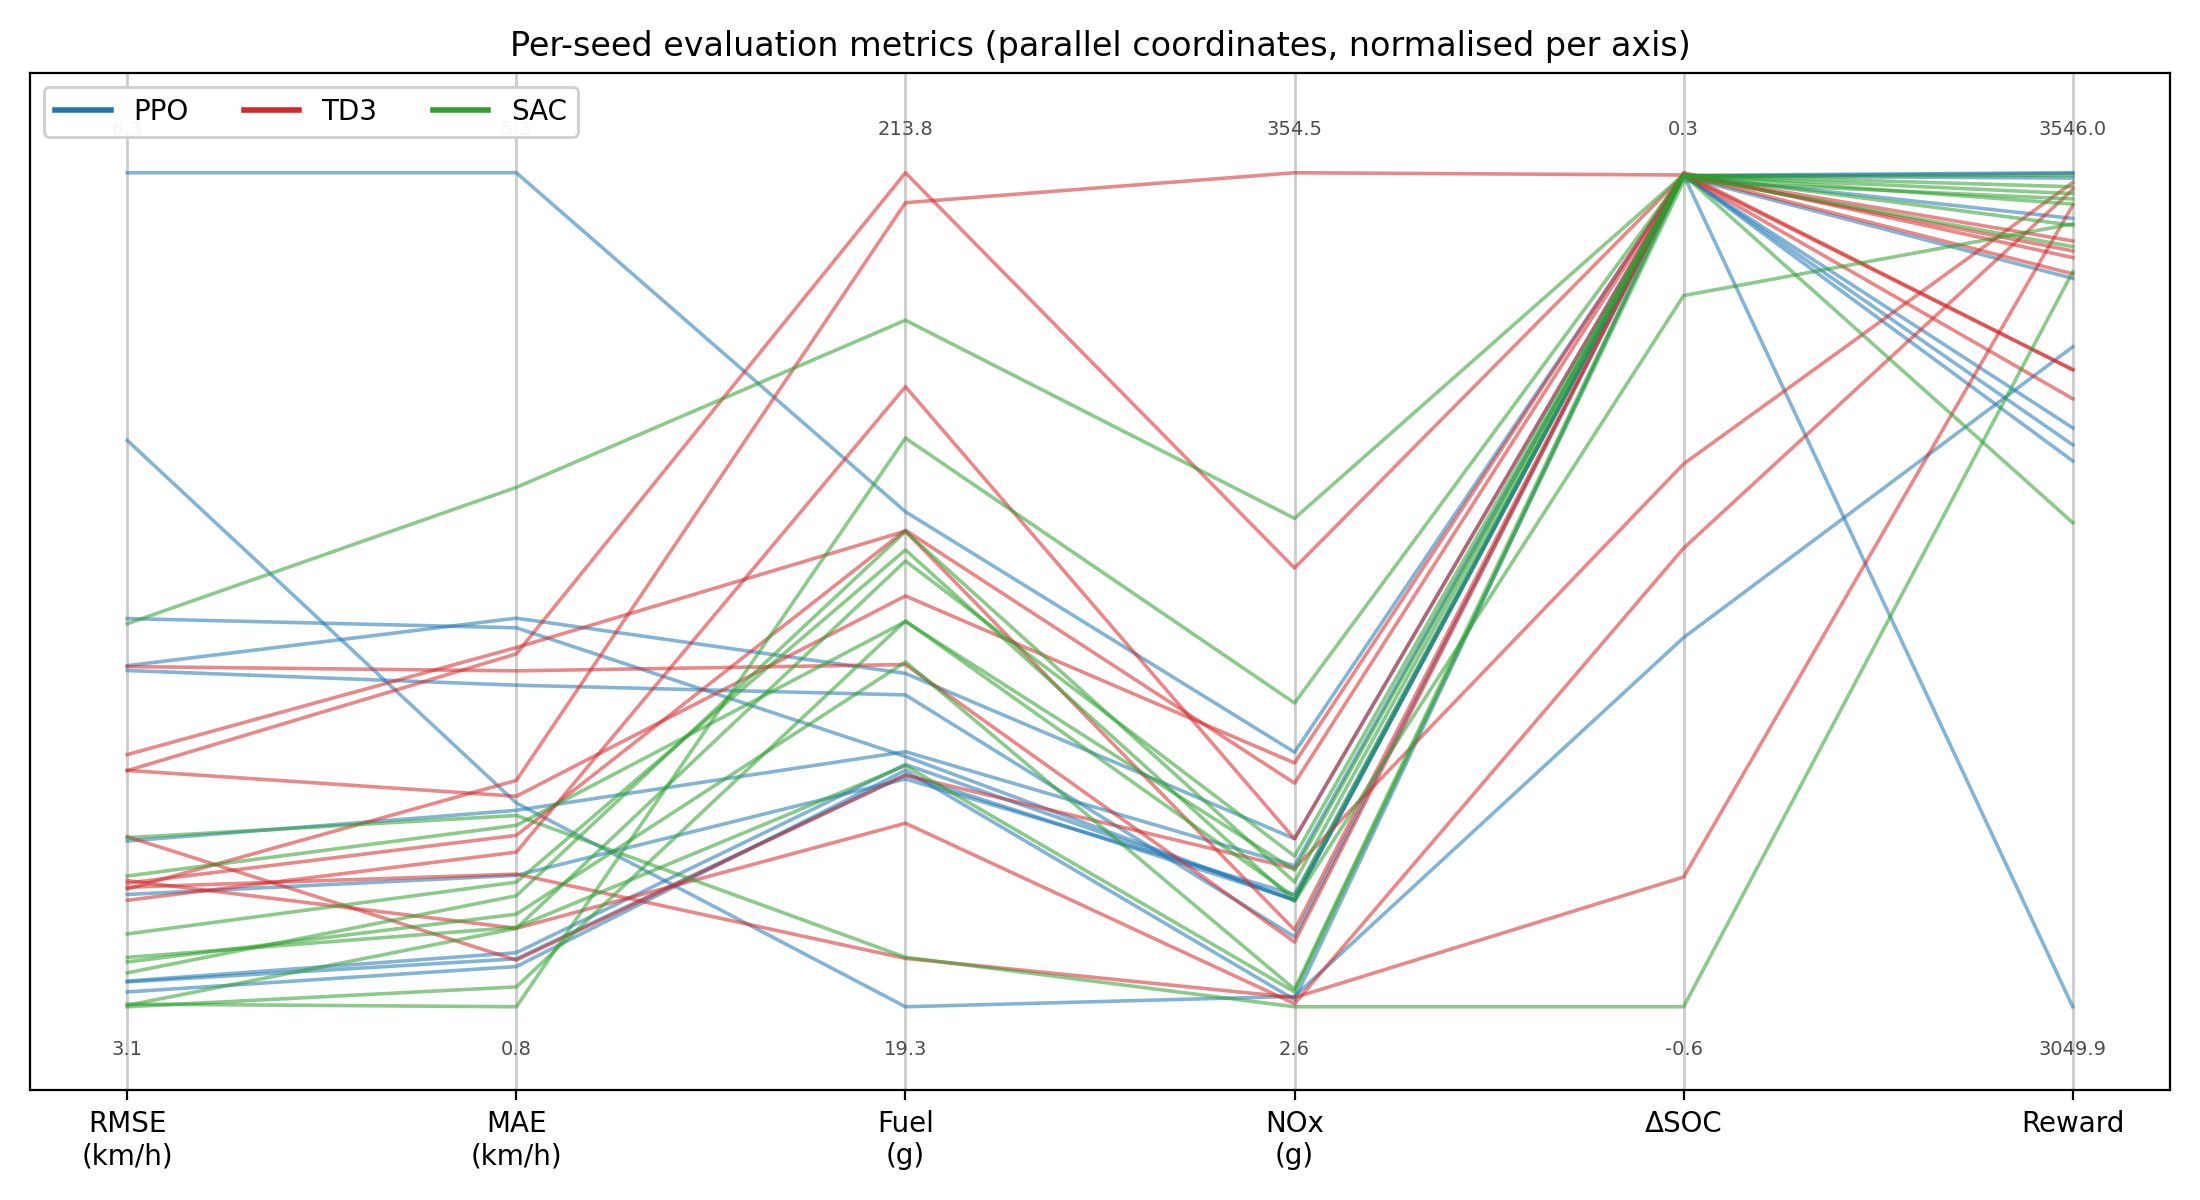
\includegraphics[width=0.7\textwidth]{imgs/analysis_plots/parallel_coords.png}
  \caption[Per-seed evaluation metrics in parallel coordinates]{Per-seed evaluation metrics in parallel coordinates. Each polyline represents one seed, each axis is normalised independently to its own min--max range with the true extrema printed at the axis ends, and colour encodes the algorithm.}
  \label{fig:phase1_parallel_coords}
\end{figure}

\paragraph{Mechanistic origin in the engine map.}
Where the Pareto and parallel-coordinate views establish \emph{that} the policies diverge, the engine-map occupancy in \autoref{fig:phase1_engine_map_occupancy} explains \emph{where} that divergence originates. Overlaying the pooled engine-on operating points on the measured EA189 \ac{BSFC} map reveals three distinct regimes: PPO and TD3 concentrate the engine near the $4{,}000$\,rpm ceiling whereas SAC spreads more broadly across low-to-mid engine speeds. None of the algorithms consistently utilises the \ac{ICE} at the most efficient measured operating point, which is consistent with the elevated fuel total. Efficiency was never rewarded, so each policy settles wherever speed tracking is convenient. The simulator additionally caps \ac{ICE} speed at $4{,}000$\,rpm, whereas the measured map extends to $4{,}500$\,rpm, leaving an unused efficiency margin. This margin is genuine headroom for Phase~2, but it must be realised by operating the engine more efficiently, not by allowing the controller to lower emissions through battery depletion.

\begin{figure}[htbp]
  \centering
  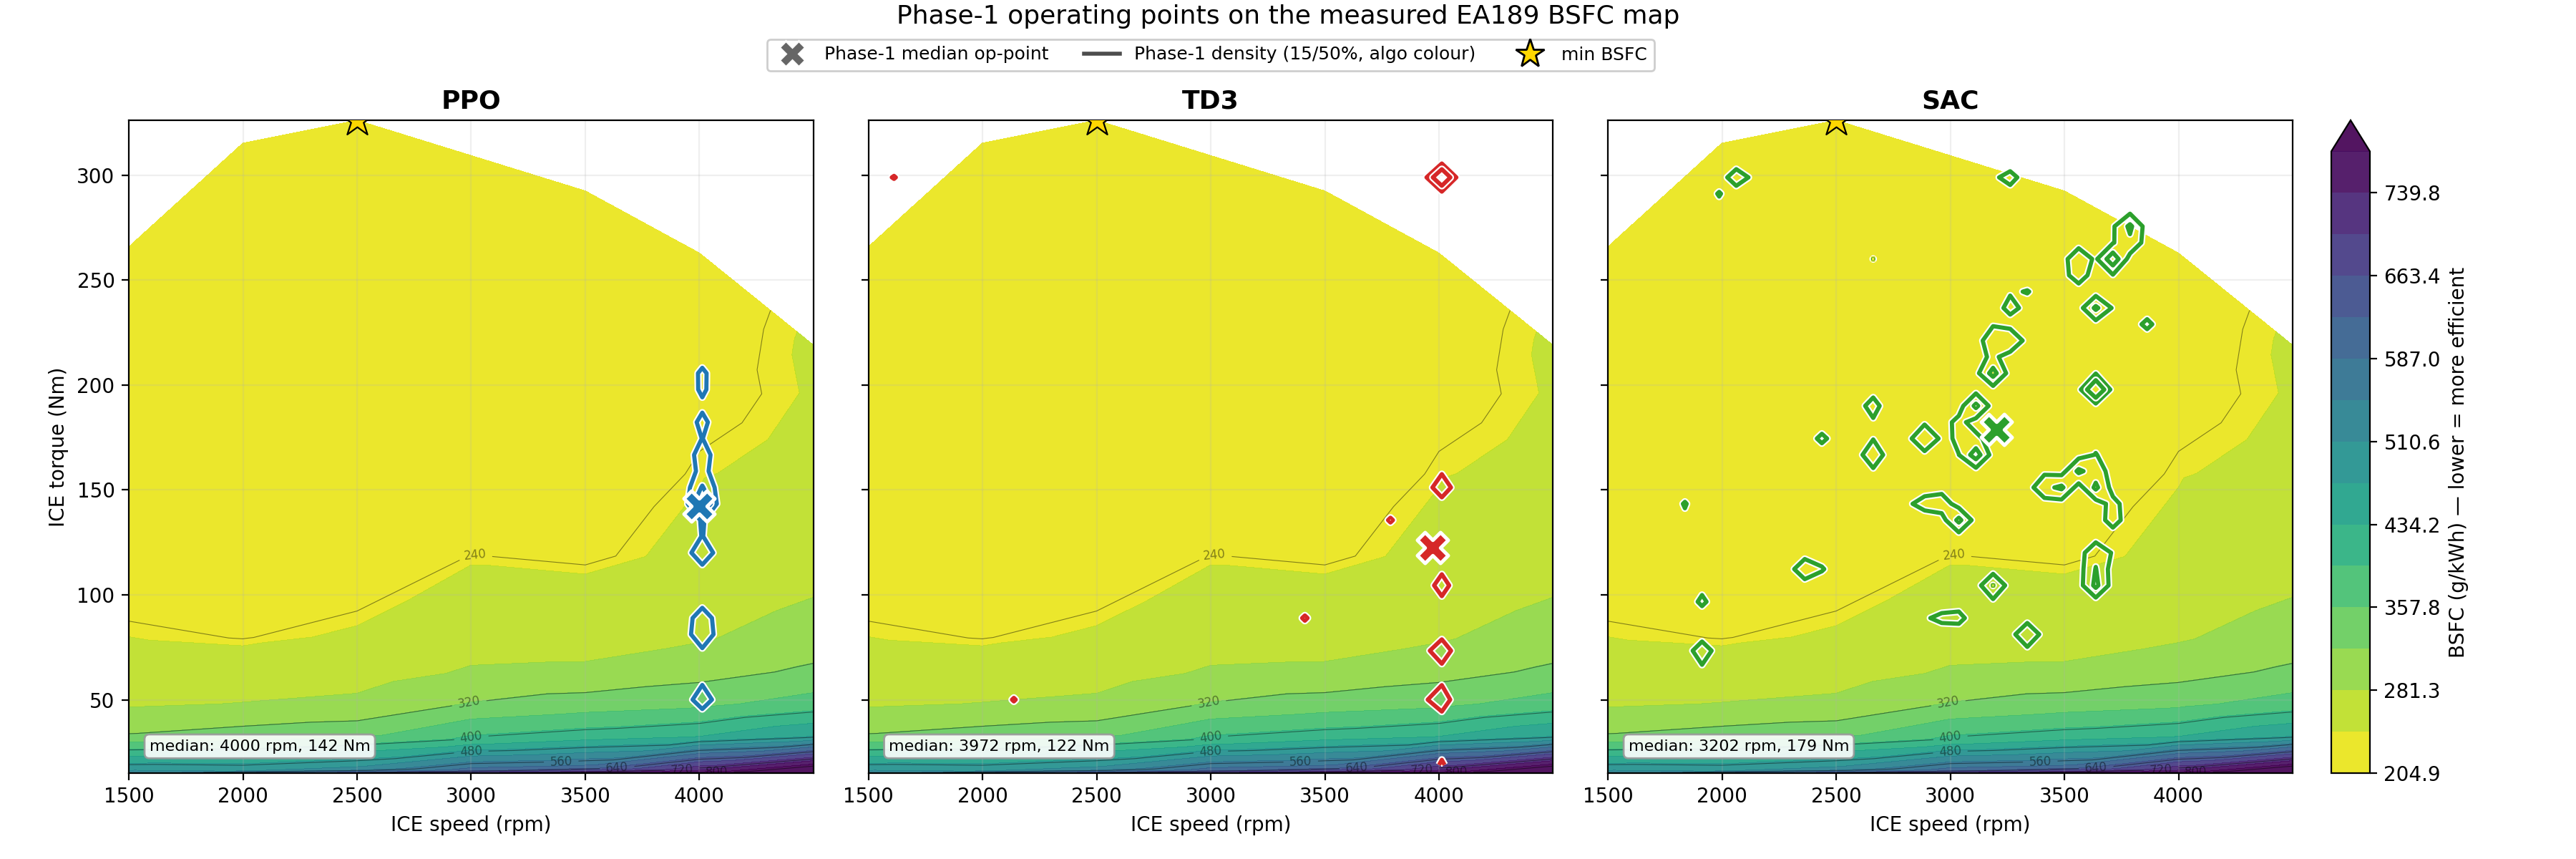
\includegraphics[width=\textwidth]{imgs/analysis_plots/engine_map_bsfc_occupancy.png}
  \caption[Learned engine operating points over the measured EA189 BSFC map]{Learned engine operating points over the measured EA189 brake-specific fuel-consumption (BSFC) map. Filled contours show the measured BSFC map, labelled black lines show iso-BSFC contours, X markers show median operating points, the gold star marks the most efficient measured point, and coloured density contours show the engine-on, positive-torque operating regions pooled over the 10 seeds of each algorithm. The two coloured contours outline where each policy spent most of its time: the inner (50\%) line encloses its most-frequented rpm--torque region, the outer (15\%) line a wider surrounding band.}
  \label{fig:phase1_engine_map_occupancy}
\end{figure}

\paragraph{Best-seed baselines and the \ac{SOC} bias.}
The checkpoint transferred to Phase~2 is selected by the lowest evaluation \ac{RMSE} within each algorithm, so the relevant reference is the concrete best-seed operating point in \autoref{tab:phase1_best_seed_action_comparison} rather than only the seed-averaged values in \autoref{tab:phase1_summary}. All three selected checkpoints saturate the battery upward with $\Delta\text{SOC}\approx+0.30$; none is charge-sustaining before the Phase~2 reward terms are introduced, which makes the battery-exploitation bias identified above an explicit property of the transferred policies, not only of the seed population. The three baselines nonetheless differ strongly in remaining headroom: PPO seed~3 is already unusually clean, SAC seed~3 is the best speed tracker but carries substantially higher \ac{NOx}, and TD3 seed~1 leaves the largest fuel- and emission-reduction margin.

\begin{table}[H]
  \centering
  \small
  \begin{tabular}{lcccccc}
    \hline
    \textbf{Algorithm} & \textbf{Seed} & \textbf{RMSE} & \textbf{MAE} & \textbf{\ac{NOx}} & \textbf{Fuel} & \textbf{$\Delta$\ac{SOC}} \\
    & & \textbf{(km/h)} & \textbf{(km/h)} & \textbf{(g)} & \textbf{(g)} & \\
    \hline
    PPO & 3 & $3.163$ & $1.001$ & $\mathbf{5.57}$ & $\mathbf{74.46}$ & $+0.299$ \\
    TD3 & 1 & $3.515$ & $1.621$ & $73.42$ & $163.94$ & $+0.300$ \\
    SAC & 3 & $\mathbf{3.106}$ & $\mathbf{0.891}$ & $48.94$ & $109.31$ & $+0.299$ \\
    \hline
  \end{tabular}
  \caption[Phase~1 best-seed comparison]{Phase~1 best seeds on the deterministic evaluation cycle. The selected seeds are the checkpoints with the lowest evaluation \ac{RMSE} per algorithm. Bold entries mark the best value in each metric. These specific seeds are used solely as the starting points for Phase~2; they are not the statistical baseline for evaluating whether Phase~2 improves speed tracking, reduces \ac{NOx}, and limits \ac{SOC} deviation. That comparison should use the 10-seed averages reported in \autoref{tab:phase1_summary}.}
  \label{tab:phase1_best_seed_action_comparison}
\end{table}

\section{Phase~2}
\label{sec:results_phase2}
Phase~2 evaluates whether the best Phase~1 speed-tracking checkpoints can be converted into charge-sustaining, low-\ac{NOx} controllers without a meaningful loss of tracking accuracy. The fine-tuning protocol follows \autoref{subsec:method_phase2} and \autoref{subsec:impl_phase2_pipeline}; the Phase~1 best-seed metrics in \autoref{tab:phase1_best_seed_action_comparison} define the concrete per-agent starting checkpoints. Because each agent is then re-trained over 10 seeds from that single checkpoint, the resulting Phase~2 10-seed statistics are compared like-for-like against the Phase~1 10-seed means of \autoref{tab:phase1_summary}; the best-seed metrics fix only the starting points and are not the statistical baseline for the comparison.

\paragraph{Augmented reward.} Phase~2 uses the reward formulation of \autoref{eq:reward} with the emission and quadratic \ac{SOC} terms active. The results below therefore vary only the two multi-objective weights $(W_{\text{emi}}, W_{\text{soc}^2})$; the speed-tracking and mechanical shaping terms remain fixed as specified in \autoref{tab:reward_weights}.

\paragraph{Weight selection by Optuna.} The two active Phase~2 weights are selected with the constrained Optuna objective defined in \autoref{eq:phase2_objective}, which minimises cumulative \ac{NOx} inside the admissible tracking and charge-drift region and penalises violations outside it. Each agent was tuned over 20 valid trials; the selected trials, scores and evaluation metrics are listed in \autoref{tab:phase2_best_trials}. The reward-weight trial histories are treated as selection diagnostics and are therefore collected in \autoref{app:phase2_reward_trial_histories}. The selected configuration was then re-trained over 10 seeds, and all reported statistics are the mean $\pm$ standard deviation over those seeds.

\begin{table}[H]
  \centering
  \small
  \begin{tabular}{@{}llrrrrrr@{}}
    \hline
    \textbf{Algorithm} & \textbf{Trial} & \textbf{$\mathbf{W_{\text{emi}}}$} & \textbf{$\mathbf{W_{\text{soc}}}$} & \textbf{Score $J$} & \textbf{\shortstack{\ac{RMSE} (km/h)}} & \textbf{\shortstack{\ac{NOx} (g)}} & \textbf{\shortstack{$\mathbf{\max|\Delta}$\ac{SOC}$|$}} \\
    \hline
    PPO & trial~1 & $1.185$ & $\phantom{0}92.86$ & $4.111$ & $\mathbf{3.16}$ & $4.11$ & $0.040$ \\
    TD3 & trial~4 & $1.010$ & $\phantom{0}64.50$ & $3.950$ & $4.01$ & $2.68$ & $0.086$ \\
    SAC & trial~4 & $0.495$ & $167.01$           & $\mathbf{2.436}$ & $3.68$ & $\mathbf{2.44}$ & $\mathbf{0.013}$ \\
    \hline
  \end{tabular}
  \caption[Best Phase~2 Optuna trials]{Best Phase~2 Optuna trial per algorithm. The Optuna score is the constrained scalar objective from \autoref{eq:phase2_objective}; lower is better and bold marks the best score. \ac{RMSE}, \ac{NOx} and $\max|\Delta\text{SOC}|$ are deterministic single-run evaluation metrics of the selected trial before 10-seed retraining.}
  \label{tab:phase2_best_trials}
\end{table}

\paragraph{Initial reward drop.} Because the fine-tune starts from a Phase~1 checkpoint whose reward normalisation and value estimates were based on the speed-only reward, the activation of the emission and \ac{SOC} penalties causes a steep drop in episodic reward in the beginning of the training before the policy re-stabilises. This is visible as the early dip in every Phase~2 learning curve of the reward-weight search.

The aggregated Phase~2 evaluation statistics across the 10 seeds per algorithm are reported in \autoref{tab:phase2_summary}. For TD3 a second column reports the statistics with its two divergent seeds removed; the reason for this split is detailed in \autoref{subsec:results_phase2_td3}.

\begin{table}[H]
  \centering
  \small
  \begin{tabular}{lcccc}
    \hline
    \textbf{Metric (evaluation cycle)} & \textbf{PPO} & \textbf{TD3 (all 10)} & \textbf{TD3 (8/10)} & \textbf{SAC} \\
    \hline
    Cumulative reward            & $3{,}553.16 \pm 2.81$ & $3{,}360.37 \pm 227.04$ & $3{,}461.38 \pm 68.14$ & $3{,}518.40 \pm 44.33$ \\
    \ac{RMSE} speed (km/h)       & $\mathbf{3.13 \pm 0.07}$ & $7.41 \pm 9.94$ & $3.96 \pm 0.47$ & $3.33 \pm 0.33$ \\
    \ac{MAE} speed (km/h)        & $\mathbf{0.80 \pm 0.08}$ & $3.66 \pm 3.75$ & $2.21 \pm 0.58$ & $1.38 \pm 0.81$ \\
    Cumulative \ac{NOx} (g)      & $4.94 \pm 0.72$ & $10.01 \pm 4.85$ & $8.65 \pm 4.43$ & $\mathbf{4.51 \pm 1.46}$ \\
    \ac{NOx} intensity (mg/km)   & $122.42$ & $252.42$ & $212.80$ & $\mathbf{111.03}$ \\
    Cumulative fuel (g)          & $\mathbf{52.76 \pm 1.25}$ & $79.79 \pm 31.40$ & $79.46 \pm 35.60$ & $63.99 \pm 20.17$ \\
    $|\Delta$\ac{SOC}$|$         & $0.029 \pm 0.004$ & $0.061 \pm 0.032$ & $0.069 \pm 0.032$ & $\mathbf{0.010 \pm 0.008}$ \\
    $\max|\Delta$\ac{SOC}$|$     & $0.038 \pm 0.009$ & $0.137 \pm 0.058$ & $0.123 \pm 0.048$ & $\mathbf{0.021 \pm 0.009}$ \\
    \hline
  \end{tabular}
  \caption[Phase~2 evaluation summary]{Phase~2 evaluation metrics across the 10 seeds of the best reward-weight configuration per algorithm. Bold marks the best value among the stable candidates (PPO and SAC); \ac{TD3} is excluded from the bold comparison due to its instability. The two \ac{TD3} columns report all 10 seeds and the statistics with the two divergent seeds (1 and 3) removed, respectively. \ac{NOx} intensity is the cumulative \ac{NOx} normalised by the $\approx 40$\,km evaluation cycle distance. Cumulative reward row is diagnostic only; since reward weights differ per algorithm, reward is not directly comparable across them.}
  \label{tab:phase2_summary}
\end{table}

\subsection{PPO}
\label{subsec:results_phase2_ppo}

\paragraph{Reward-weight search.}
\ac{PPO}'s Optuna study ran $20$ valid trials ($16$ completed, $4$ pruned) and settled on the highest emission weight of the three agents, $W_{\text{emi}} = 1.185$, with a moderate $W_{\text{soc}^2} = 92.86$ (\autoref{tab:phase2_best_trials}). The corresponding reward-weight trial history is provided in \autoref{fig:phase2_ppo_reward_trials}. Overall, this produced the agent with the tightest speed-tracking ability with a \ac{RMSE} of $3.16$.

\begin{figure}[htbp]
  \centering
  
\includegraphics[width=0.75\textwidth]{imgs/plots/phase2/ppo/training_progress.png}
  \caption[PPO seed training in Phase~2]{Training progress across the 10 PPO seeds in Phase~2. Curves are smoothed via moving average over 80 episodes, and the y-axis is clipped to $\pm4000$.}
  \label{fig:phase2_ppo_seeds}
\end{figure}

\begin{figure}[htbp]
  \centering
  
\includegraphics[width=0.7\textwidth]{imgs/plots/phase2/ppo/eval_speed_tracking.png}
  \caption[PPO speed tracking in Phase~2]{Evaluation speed-tracking trajectory for PPO in Phase~2.}
  \label{fig:phase2_ppo_eval_rmse_tracking}
\end{figure}

\paragraph{Seed runs.}
PPO is the most reliable agent in Phase~2. After the initial reward shock, all $10$ seeds recover to nearly identical learning curves (\autoref{fig:phase2_ppo_seeds}) and the evaluation \ac{RMSE} collapses to $3.13 \pm 0.07$\,km/h --- below the Phase~1 $10$-seed mean of $4.19$\,km/h, and with a per-seed standard deviation more than an order of magnitude tighter than the $0.98$\,km/h of Phase~1. The speed-tracking trajectory in \autoref{fig:phase2_ppo_eval_rmse_tracking} is essentially indistinguishable from the Phase~1 PPO baseline, while the evaluation metrics in \autoref{tab:phase2_summary} show the energy side transformed: mean cumulative \ac{NOx} falls to $4.94 \pm 0.72$\,g (from the Phase~1 10-seed mean of $48.3$\,g) and fuel to $52.76 \pm 1.25$\,g (from $79.6$\,g), and the charge drift tightens to $|\Delta\text{SOC}| = 0.029$ from the Phase~1 10-seed mean of $+0.247$. PPO therefore converts an already-clean but battery-saturating Phase~1 policy into a clean and charge-sustaining one at no cost to tracking accuracy.

\paragraph{The best seed.}
The best Phase~2 PPO seed is seed~4 with a composite score $J$ of $4.23$. This value is determined by the \ac{NOx} term only, since the \ac{SOC} and \ac{RMSE} constraints are satisfied.

The policy preserves the main qualitative features of the Phase~1 PPO strategy: the engine remains continuously on, the \ac{ICE} speed still saturates at $4{,}000$\,rpm, and mechanical braking is avoided. The difference lies in the \ac{EM2} and fuel commands, both of which become more volatile. During the second, third, fifth, and sixth phases of the evaluation cycle, the \ac{EM2} torque rapidly switches between approximately $-340$ and $421$\,Nm. The density plot therefore forms three clusters: the two torque extremes and an additional cluster around $50$\,Nm. The fuel-injection command also broadens around $20$\,mg and now spans roughly $0$--$20$\,mg, showing similarly volatile behaviour. These results suggest that the more aggressive torque and fuel modulation is part of the mechanism by which PPO reduces \ac{NOx} substantially. Provided that these commands are mechanically feasible and that the surrogate models remain reliable in this operating regime, this behaviour may offer useful insight; however, mechanical feasibility is not validated within the scope of this thesis.

The resulting velocity, \ac{SOC}, and tailpipe \ac{NOx} emissions are depicted in \autoref{fig:phase2_ppo_seed4_evaluation_results}.

\begin{figure}[H]
  \centering
  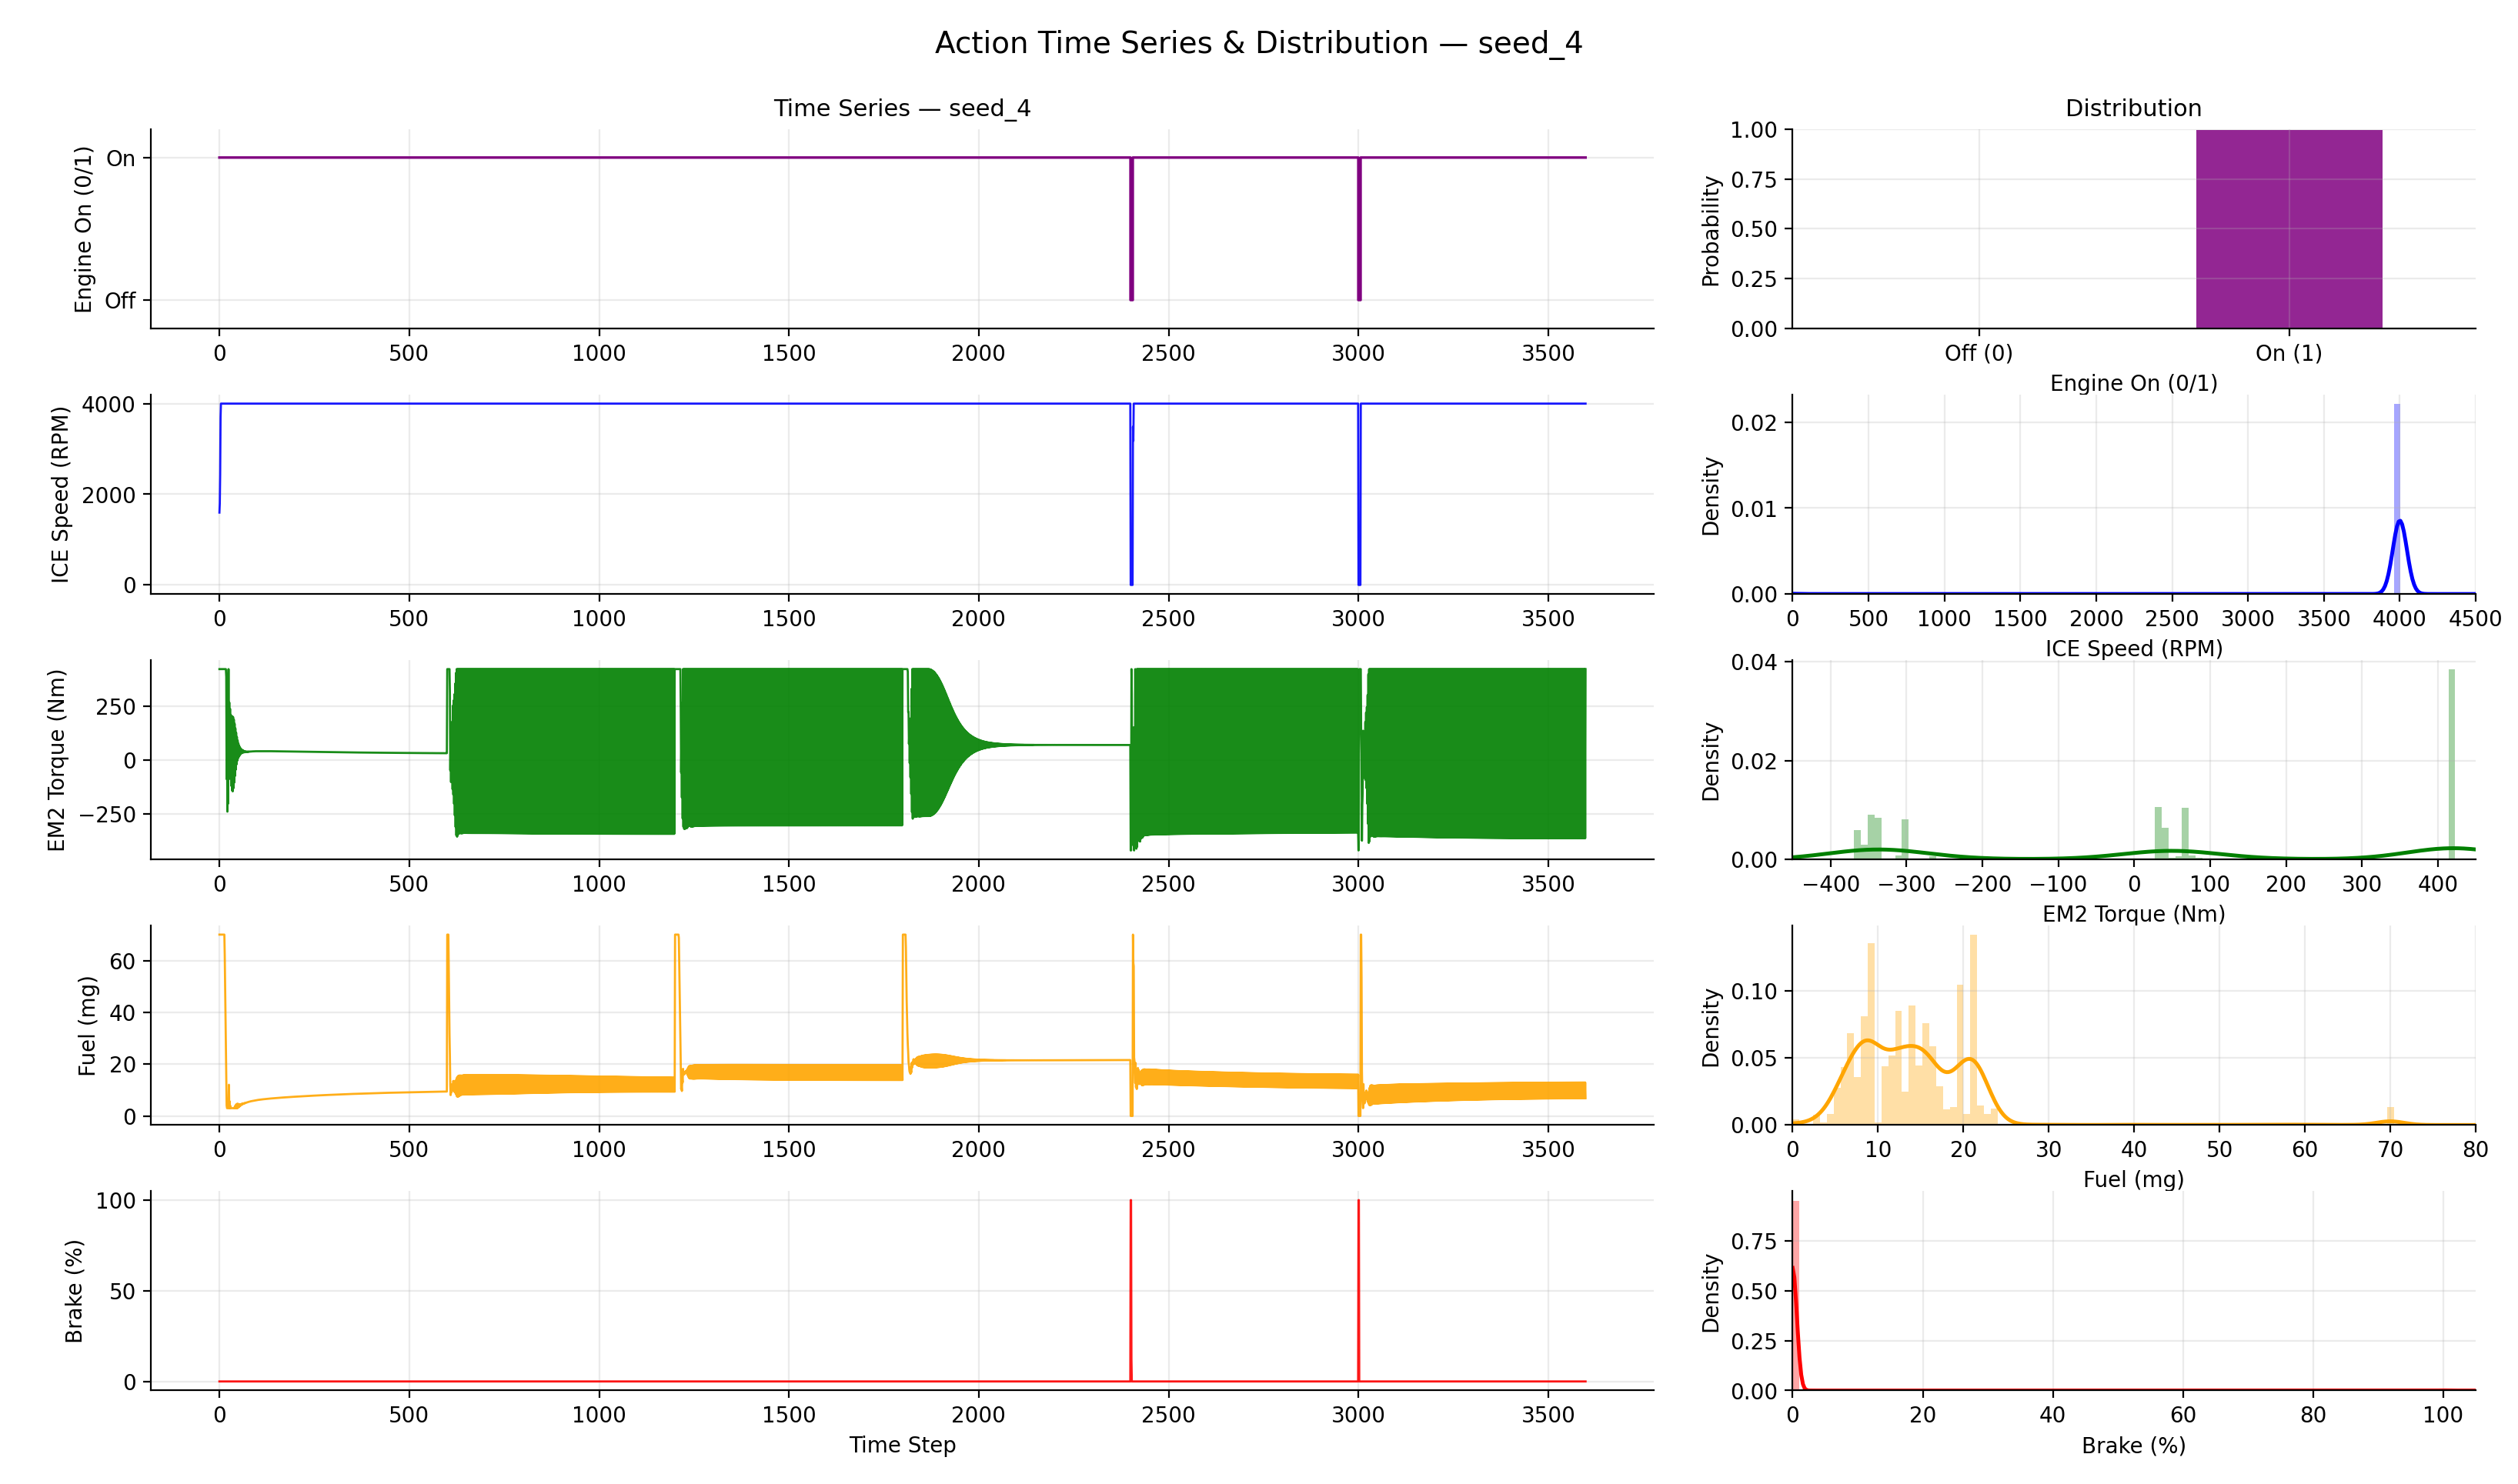
\includegraphics[width=\textwidth]{imgs/plots/phase2/ppo/seed_4_action_summary.png}
  \caption[Best PPO seed action summary in Phase~2]{Action summary for the best PPO checkpoint, seed~4, in Phase~2. The left panels show the PPO agent's actions during the evaluation cycle; the right panels show the corresponding densities.}
  \label{fig:phase2_ppo_action_summary}
\end{figure}

\begin{figure}[H]
  \centering
  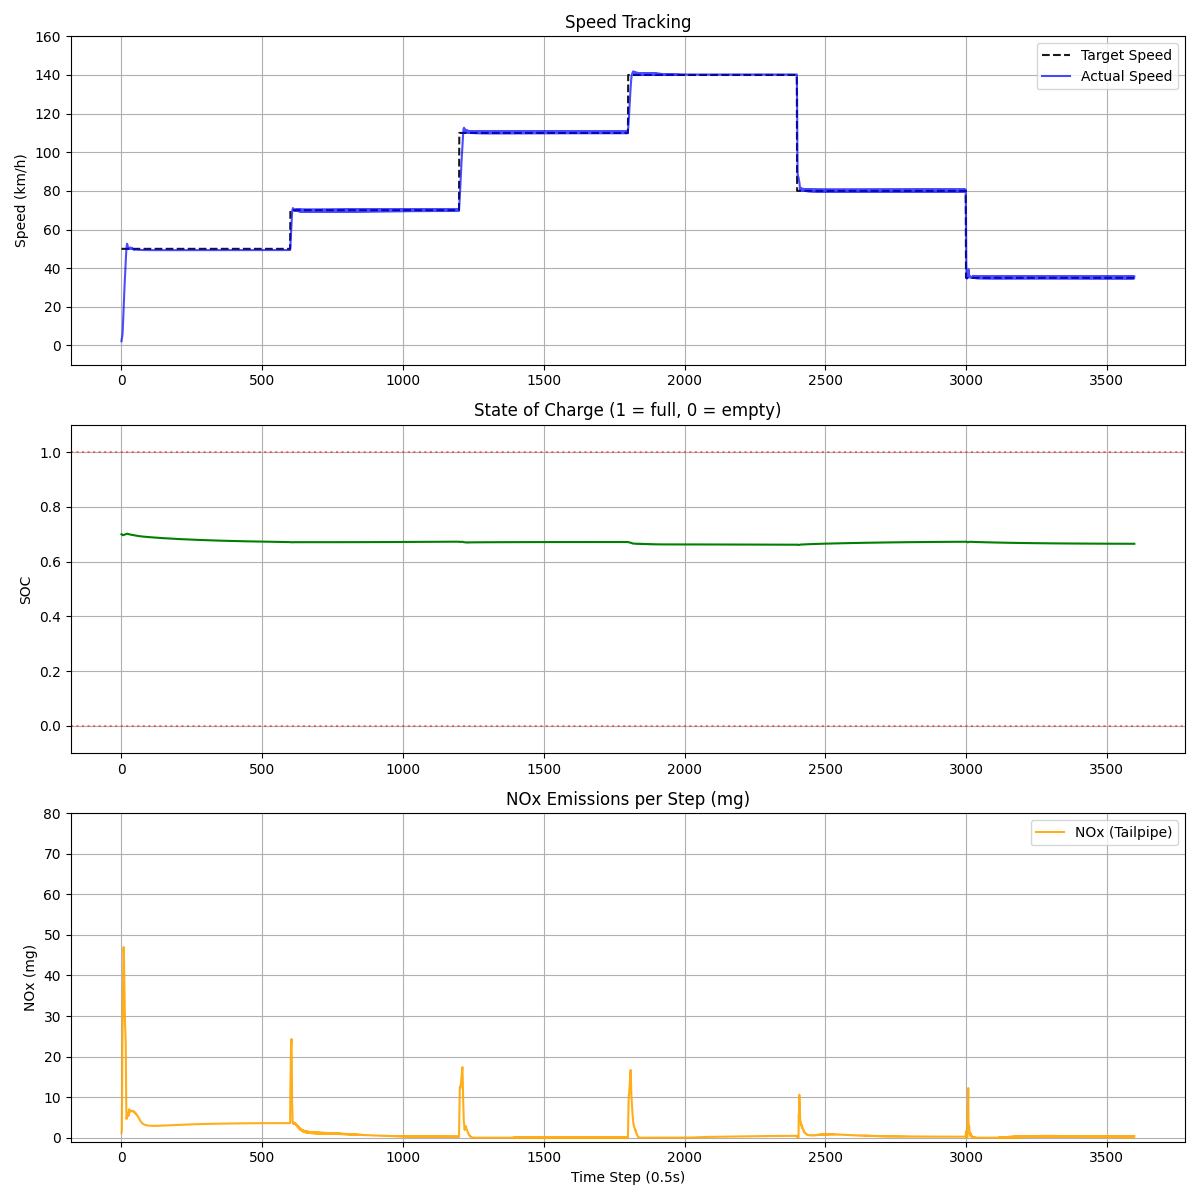
\includegraphics[width=0.55\textwidth]{imgs/plots/phase2/ppo/seed_4_evaluation_results.png}
  \caption[Best PPO seed evaluation results in Phase~2]{Evaluation results for the best PPO checkpoint, seed~4, in Phase~2. The panels show speed tracking, the \ac{SOC} trajectory, and tailpipe \ac{NOx} emissions over the evaluation cycle.}
  \label{fig:phase2_ppo_seed4_evaluation_results}
\end{figure}

\subsection{TD3}
\label{subsec:results_phase2_td3}

\paragraph{Reward-weight search.}
TD3's study ran $20$ valid trials ($15$ completed, $5$ pruned) and selected the lowest \ac{SOC} weight of the three agents, $W_{\text{soc}^2} = 64.50$, paired with a high emission weight $W_{\text{emi}} = 1.010$. The comparably low \ac{SOC} weight leads to the largest residual drift of the three agents ($\max|\Delta\text{SOC}| = 0.086$, \autoref{tab:phase2_best_trials}). The corresponding reward-weight trial history is provided in \autoref{fig:phase2_td3_reward_trials}.

\begin{figure}[htbp]
  \centering
  
\includegraphics[width=0.75\textwidth]{imgs/plots/phase2/td3/training_progress.png}
  \caption[TD3 seed training in Phase~2]{Training progress across the 10 TD3 seeds in Phase~2. Curves are smoothed via moving average over 80 episodes, and the y-axis is clipped to $\pm4000$; the large-amplitude reward collapses persist throughout training.}
  \label{fig:phase2_td3_seeds}
\end{figure}

\begin{figure}[htbp]
  \centering
  
\includegraphics[width=0.7\textwidth]{imgs/plots/phase2/td3/eval_speed_tracking.png}
  \caption[TD3 speed tracking in Phase~2]{Evaluation speed-tracking trajectory for TD3 in Phase~2. The spread across seeds is far larger than for PPO or SAC.}
  \label{fig:phase2_td3_eval_rmse_tracking}
\end{figure}

\paragraph{Seed runs.}
TD3 does not produce a stable controller in Phase~2. Its seed-wise learning curves (\autoref{fig:phase2_td3_seeds}) exhibit large-amplitude reward collapses that occur throughout the full $4{,}000{,}000$-step budget rather than dying out after the initial reward shock. Two of the ten seeds (1 and 3) never recover a usable speed-tracking policy: seed~3 gets stuck at a low-speed plateau and never follows the higher staircase setpoints, reaching $35.57$\,km/h \ac{RMSE}, and seed~1 is a milder version of the same failure at $6.78$\,km/h. These two seeds inflate the all-seed \ac{RMSE} to $7.41 \pm 9.94$\,km/h; removing them recovers a mean of $3.96 \pm 0.47$\,km/h (\autoref{tab:phase2_summary}, third column), comparable to SAC. However, the volatility in \autoref{fig:phase2_td3_seeds} is present in \emph{all} seeds, not only the two that diverge, so even the surviving runs cannot be considered robust and reliable. \textbf{TD3 is therefore not considered a viable candidate for the control problem}, and the favourable $8/10$ column is reported only to characterise the failure rather than to reclaim the agent's competence.

\paragraph{Best-seed analysis omitted.}
The analogous best-seed action-summary and evaluation-result panels are omitted for TD3. Although the scalar selection score would nominate seed~9, the Phase~2 TD3 population is unstable and includes outright failed policies; interpreting a single surviving checkpoint would therefore overstate the reliability of the algorithm.

\subsection{SAC}
\label{subsec:results_phase2_sac}

\paragraph{Reward-weight search.}
SAC's study ran $20$ valid trials ($11$ completed, $9$ pruned) and produced the cleanest single trial of the entire Phase~2 search ($2.44$\,g \ac{NOx} at $\max|\Delta\text{SOC}| = 0.013$, \autoref{tab:phase2_best_trials}). It selected a moderate emission weight ($W_{\text{emi}} = 0.495$) but the highest \ac{SOC} weight of the three agents ($W_{\text{soc}^2} = 167.01$). The corresponding reward-weight trial history is provided in \autoref{fig:phase2_sac_reward_trials}. This is consistent with SAC carrying the larger \ac{NOx} reduction burden among the two stable agents: its transferred checkpoint ($48.94$\,g \ac{NOx}, \autoref{tab:phase1_best_seed_action_comparison}) emitted substantially more than PPO's ($5.57$\,g).

\begin{figure}[htbp]
  \centering
  
\includegraphics[width=0.75\textwidth]{imgs/plots/phase2/sac/training_progress.png}
  \caption[SAC seed training in Phase~2]{Training progress across the 10 SAC seeds in Phase~2. Curves are smoothed via moving average over 80 episodes, and the y-axis is clipped to $\pm4000$.}
  \label{fig:phase2_sac_seeds}
\end{figure}

\begin{figure}[htbp]
  \centering
  
\includegraphics[width=0.7\textwidth]{imgs/plots/phase2/sac/eval_speed_tracking.png}
  \caption[SAC speed tracking in Phase~2]{Evaluation speed-tracking trajectory for SAC in Phase~2.}
  \label{fig:phase2_sac_eval_rmse_tracking}
\end{figure}

\paragraph{Seed runs.}
SAC achieves the largest absolute and relative emission reduction. Its learning curves (\autoref{fig:phase2_sac_seeds}) are stabilising after the initial shock, and the evaluation \ac{RMSE} of $3.33 \pm 0.33$\,km/h is slightly better than its Phase~1 10-seed mean of $3.45$\,km/h. The energy-side metrics in \autoref{tab:phase2_summary} show cumulative \ac{NOx} cut by $93\%$ against the Phase~1 10-seed mean of $63.8$\,g to $4.51 \pm 1.46$\,g --- the lowest mean of the three agents --- and the charge drift reduced to $|\Delta\text{SOC}| = 0.010$ (from the Phase~1 10-seed mean of $+0.191$), roughly three times tighter than PPO's $0.029$.

\paragraph{The best seed.}
The best Phase~2 SAC seed is seed~7 with a composite score $J$ of $2.06$. As for the selected PPO seed, the score is determined by the \ac{NOx} term because the \ac{SOC} and \ac{RMSE} constraints are satisfied. The corresponding action summary and evaluation results are shown in \autoref{fig:phase2_sac_action_summary} and \autoref{fig:phase2_sac_seed7_evaluation_results}, respectively.

SAC's braking and engine on/off behaviour remains largely unchanged compared with Phase~1. The \ac{ICE} speed, however, shifts to lower operating points, with one cluster around $2{,}400$\,rpm and another around $1{,}000$\,rpm during the first stage of the evaluation cycle. A volatile pattern similar to that of PPO is visible in the \ac{EM2} command, which produces a wider density distribution. Stages~2--5 contribute most strongly to this effect, with the command rapidly switching between approximately $-180$ and $250$\,Nm. The fuel command also shifts downward: its main density peak is now around $15$\,mg rather than approximately $35$\,mg in Phase~1. This suggests that the same increase in command volatility already observed for PPO in Phase~2 contributes to SAC's substantial \ac{NOx} reduction. Whether this behaviour reflects a transferable control insight or an exploitation of the surrogate system cannot be determined within the scope of this thesis.

The resulting velocity, \ac{SOC}, and tailpipe \ac{NOx} emissions are depicted in \autoref{fig:phase2_sac_seed7_evaluation_results}.

\begin{figure}[H]
  \centering
  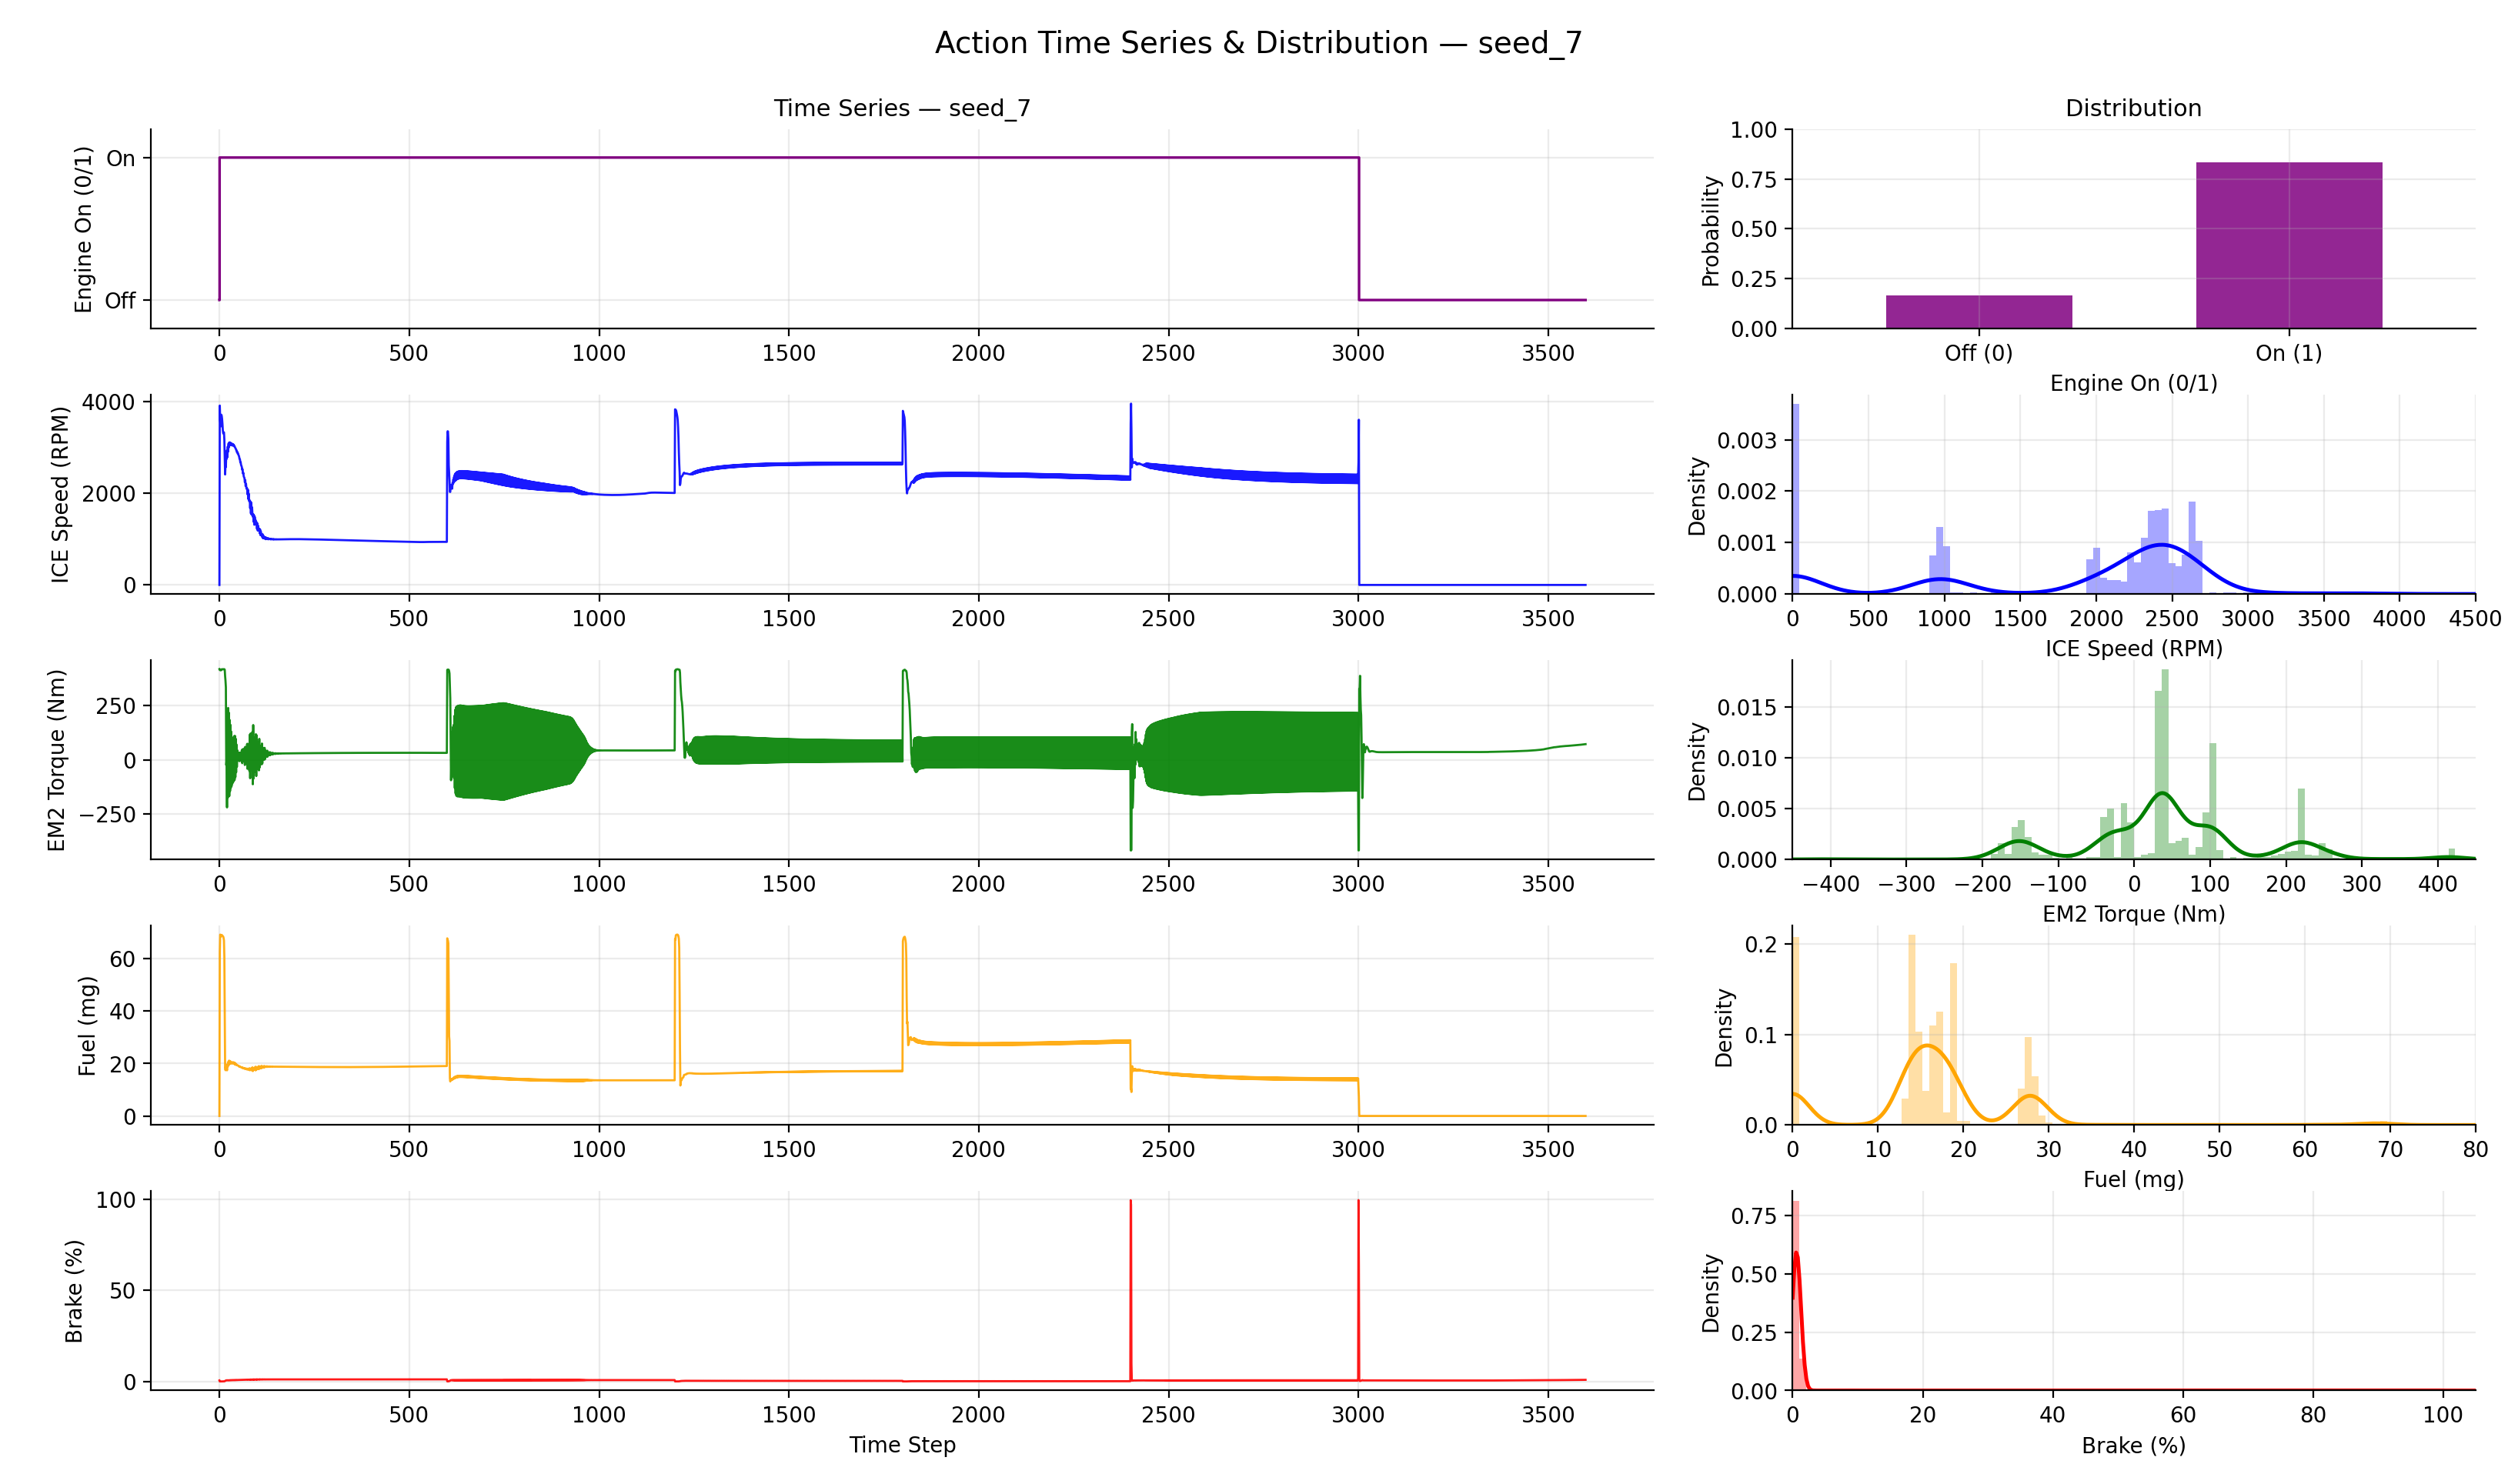
\includegraphics[width=\textwidth]{imgs/plots/phase2/sac/seed_7_action_summary.png}
  \caption[Best SAC seed action summary in Phase~2]{Action summary for the best SAC checkpoint, seed~7, in Phase~2. The left panels show the SAC agent's actions during the evaluation cycle; the right panels show the corresponding densities.}
  \label{fig:phase2_sac_action_summary}
\end{figure}

\begin{figure}[H]
  \centering
  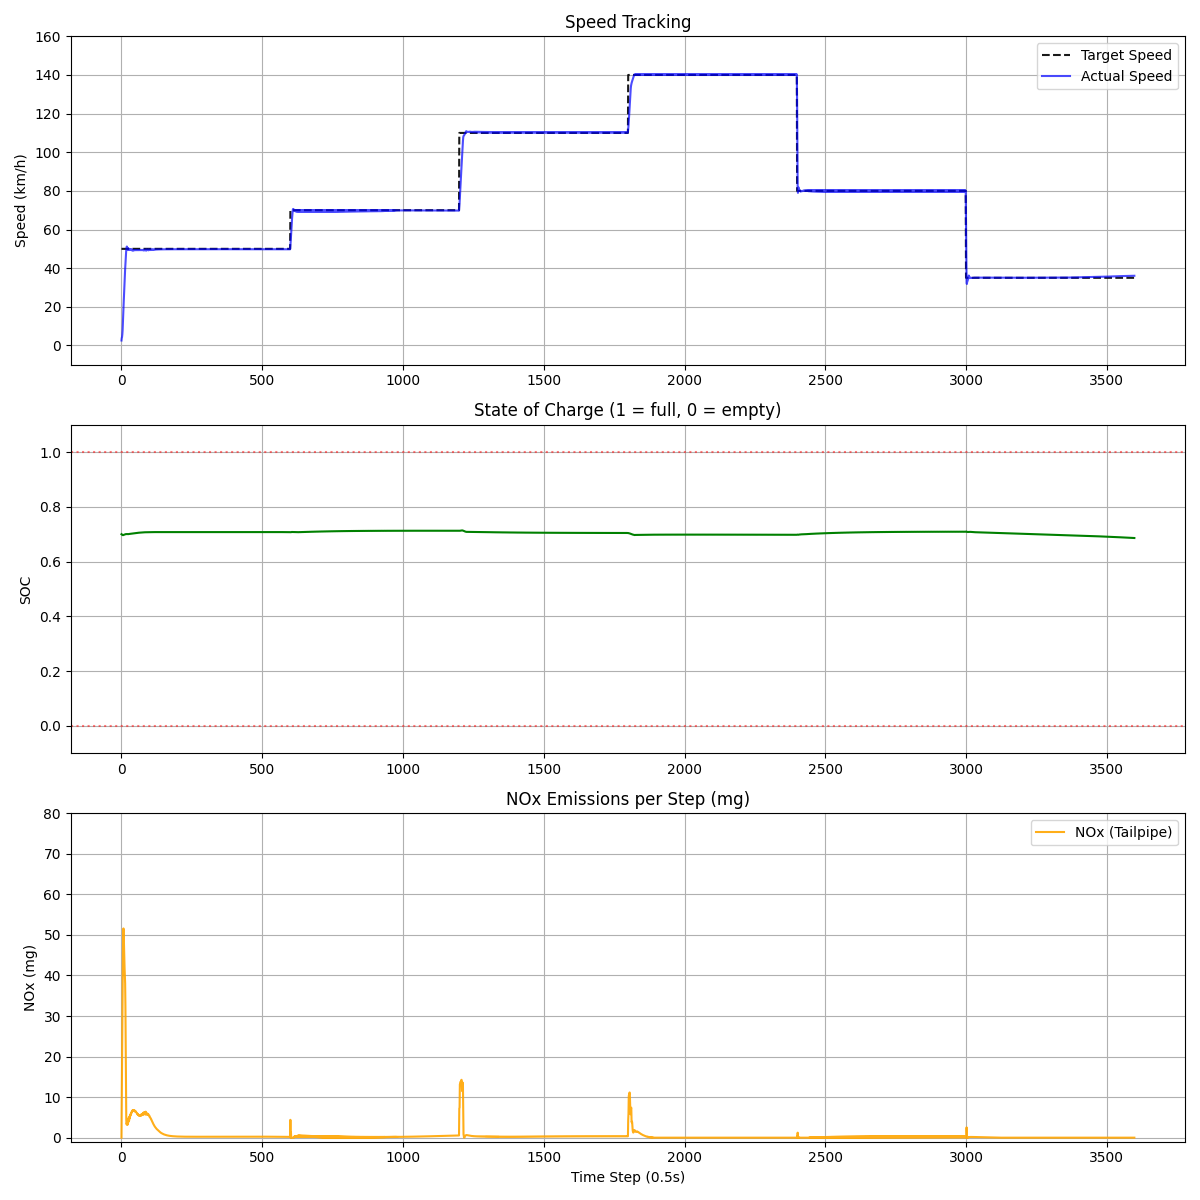
\includegraphics[width=0.55\textwidth]{imgs/plots/phase2/sac/seed_7_evaluation_results.png}
  \caption[Best SAC seed evaluation results in Phase~2]{Evaluation results for the best SAC checkpoint, seed~7, in Phase~2. The panels show speed tracking, the \ac{SOC} trajectory, and tailpipe \ac{NOx} emissions over the evaluation cycle.}
  \label{fig:phase2_sac_seed7_evaluation_results}
\end{figure}

\subsection{Summary}
\label{subsec:results_phase2_summary}

\paragraph{Training convergence.}
As discussed above, the Phase~2 results reveal clear differences in control performance across the algorithms. This pattern is also apparent in the seed-averaged training trajectories used to assess convergence. \autoref{fig:phase2_training_progress_comparison} aggregates the 10-seed training performance for each algorithm and shows that \ac{TD3} fails to converge to a robust policy, whereas \ac{PPO} and \ac{SAC} stabilise and eventually reach episodic rewards close to those observed in Phase~1.

\begin{figure}[H]
  \centering
  
\includegraphics[width=0.7\textwidth]{imgs/plots/phase2/training_progress_comparison.png}
  \caption[Phase~2 training-progress comparison]{Comparison of seed-averaged training progress across all Phase~2 algorithms. Curves are smoothed with a moving average over 80 episodes, y-axis clipped to $\pm4000$ and shaded bands represent $\pm$ one standard deviation across the 10 seed curves at each x-grid point.}
  \label{fig:phase2_training_progress_comparison}
\end{figure}

\paragraph{Multi-objective feasibility.}
Activating the emission and \ac{SOC} reward terms and fine-tuning from the Phase~1 checkpoints reduces cumulative \ac{NOx} and the \ac{SOC} drift by roughly an order of magnitude (when neglecting TD3). Comparing the 10-seed statistics with the Phase~1 10-seed mean (\autoref{tab:phase1_summary}): mean speed tracking is not degraded but slightly improved for the two stable agents (PPO $4.19 \to 3.13$, SAC $3.45 \to 3.33$\,km/h), with the its \ac{RMSE} variance reduced. The per-agent change against these Phase~1 10-seed baselines is summarised in \autoref{tab:phase2_headline}.

\begin{table}[H]
  \centering
  \small
  \begin{tabular}{lccc}
    \hline
    \textbf{Metric} & \textbf{PPO} & \textbf{TD3 (8/10)} & \textbf{SAC} \\
    \hline
    \ac{RMSE} (km/h)     & $4.19 \to 3.13$ & $3.81 \to 3.96$ & $3.45 \to 3.33$ \\
    \ac{RMSE} $\sigma$   & $0.98 \to \mathbf{0.07}$ & $0.29 \to 0.47$ & $0.43 \to 0.33$ \\
    \ac{NOx} (g)         & $48.3 \to \mathbf{4.94}$ & $95.4 \to 8.65$ & $63.8 \to \mathbf{4.51}$ \\
    \ac{NOx} (mg/km)     & $1{,}165 \to 122$ & $2{,}327 \to 213$ & $1{,}564 \to 111$ \\
    Fuel (g)             & $79.6 \to 52.8$ & $122.6 \to 79.5$ & $113.5 \to 64.0$ \\
    $|\Delta$\ac{SOC}$|$ & $0.247 \to \mathbf{0.029}$ & $0.146 \to 0.069$ & $0.191 \to \mathbf{0.010}$ \\
    \hline
  \end{tabular}
  \caption[Phase~1 to Phase~2 headline changes]{Phase~1 $\to$ Phase~2 change per algorithm. Phase~1 figures are the 10-seed means from \autoref{tab:phase1_summary}; Phase~2 figures are from \autoref{tab:phase2_summary} (TD3 with the two divergent seeds removed). \ac{NOx} and fuel fall together because the Phase~1 policies burned extra fuel at high engine load purely to overcharge the battery, an effect the \ac{SOC} term removes.}
  \label{tab:phase2_headline}
\end{table}

The overall progression of this reduction across the full training pipeline is shown in \autoref{fig:nox_pipeline}, which traces the per-agent mean cumulative \ac{NOx} from the Phase~1 baseline through the two reward-weight search stages to the Phase~2 fine-tune. PPO and SAC settle just above the indicative Euro~6 line at $\approx\!5$\,g per cycle, whereas TD3 plateaus at ($10$\,g).

\begin{figure}[H]
  \centering
  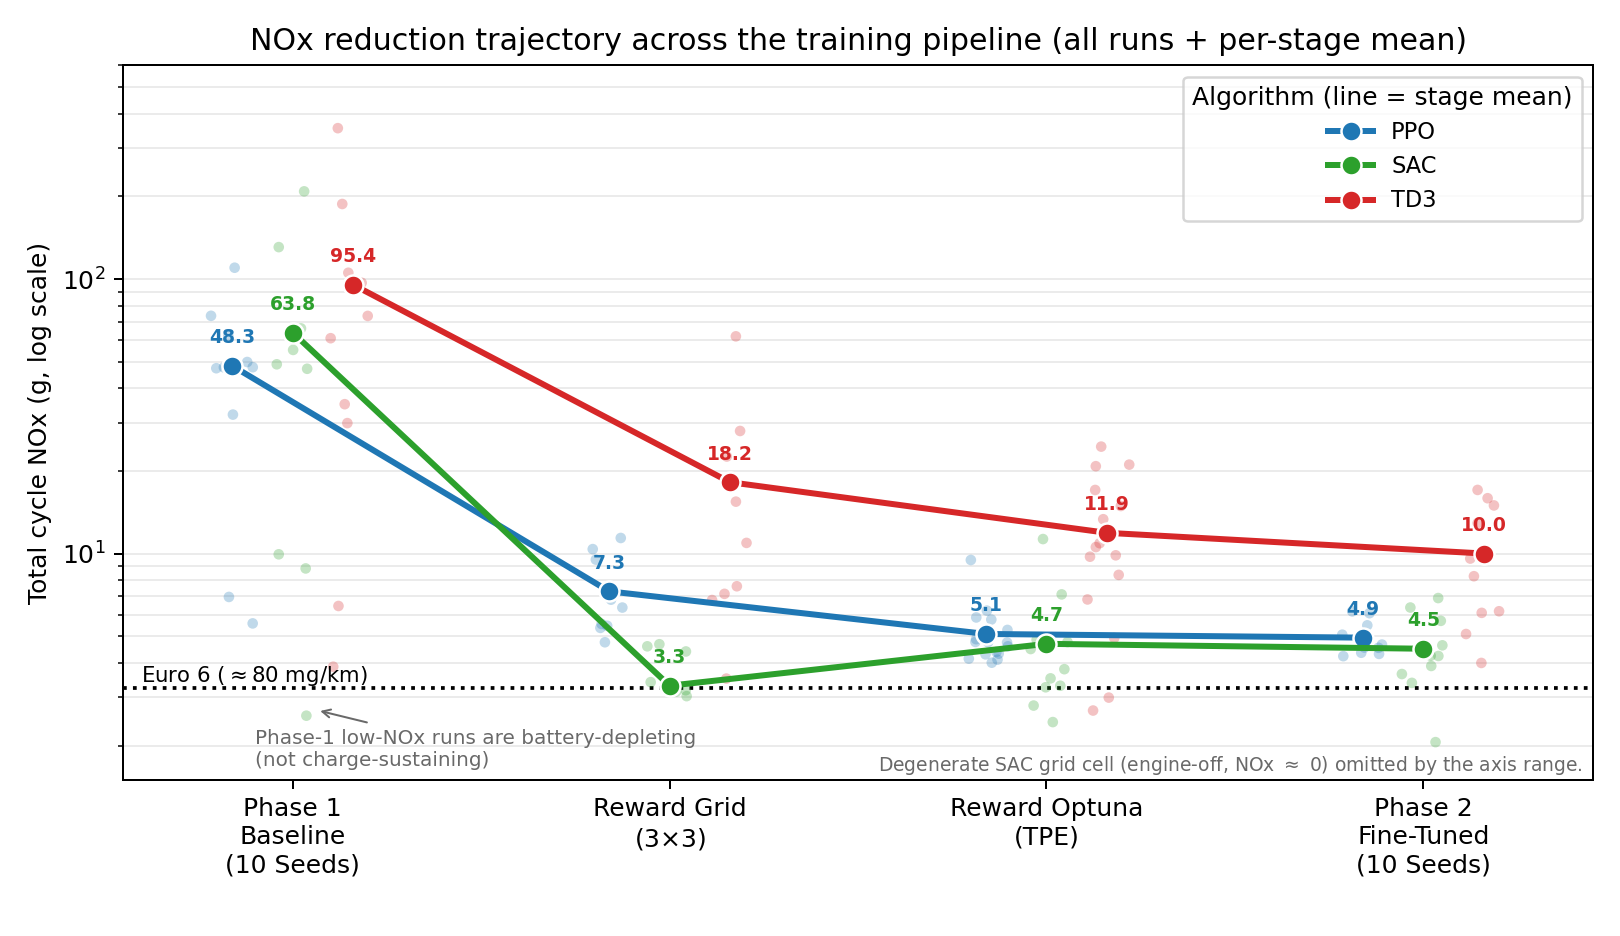
\includegraphics[width=0.7\textwidth]{imgs/nox_pipeline_swarm_traj.png}
  \caption[NO\textsubscript{x} reduction across the training pipeline]{Per-stage cumulative tail-pipe \ac{NOx} (total grams over the identical staircase evaluation cycle, logarithmic y-axis) across the four pipeline stages: the Phase~1 baseline ($10$ seeds, emission term off), the $3\times3$ reward-weight grid, the Optuna \ac{TPE} refinement, and the Phase~2 10-seed fine-tuned. Faint markers denote individual runs; the bold line connects the per-stage mean of each algorithm. The dotted line marks the gram-equivalent of the Euro~6 limit ($80$\,mg/km over the ${\approx}40.4$\,km cycle). Note that the grid and Optuna stages hold one run per weight configuration, so their means are not a controlled comparison against the 10-seed Phase~1/Phase~2 statistics; the single degenerate engine-off \ac{SAC} grid cell (\ac{NOx}~${\approx}\,0$) lies below the axis range and is the reason why \ac{NOx} for SAC in that experimental stage is so low.}
  \label{fig:nox_pipeline}
\end{figure}

\paragraph{Resolving the Phase~1 charge--emissions trade-off.}
The Phase~2 parallel-coordinate plot in \autoref{fig:phase2_parallel_coords} shows that the scatter observed in Phase~1 (\autoref{fig:phase1_parallel_coords}) is replaced by a much more coherent low-emission, charge-sustaining bundle. In Phase~1, the tracking axes (\ac{RMSE}, \ac{MAE}) were already tightly clustered, but fuel, \ac{NOx}, and $\Delta$\ac{SOC} spanned more than two orders of magnitude. Phase~2 removes this degeneracy: $\Delta$\ac{SOC} contracts to a narrow band around zero for every seed, \ac{NOx} shrinks from a $2.6$--$354$\,g span to roughly $2$--$17$\,g, and fuel tightens correspondingly. For PPO (blue) and SAC (green), the polylines now remain compact across all six axes, meaning that seeds which track well are also clean and \ac{SOC}-maintaining; the only remaining crossings and spikes are the volatile TD3 seeds, which jump on fuel and \ac{NOx} and collapse on reward. The Pareto overlay in \autoref{fig:phase2_pareto_overlay} highlights that only one Phase~1 seed is charge-sustaining ($|\Delta\text{SOC}| < 0.10$), and it still emits $60.9$\,g of \ac{NOx}, whereas all Phase~2 seeds are charge-sustaining.

\begin{figure}[htbp]
  \centering
  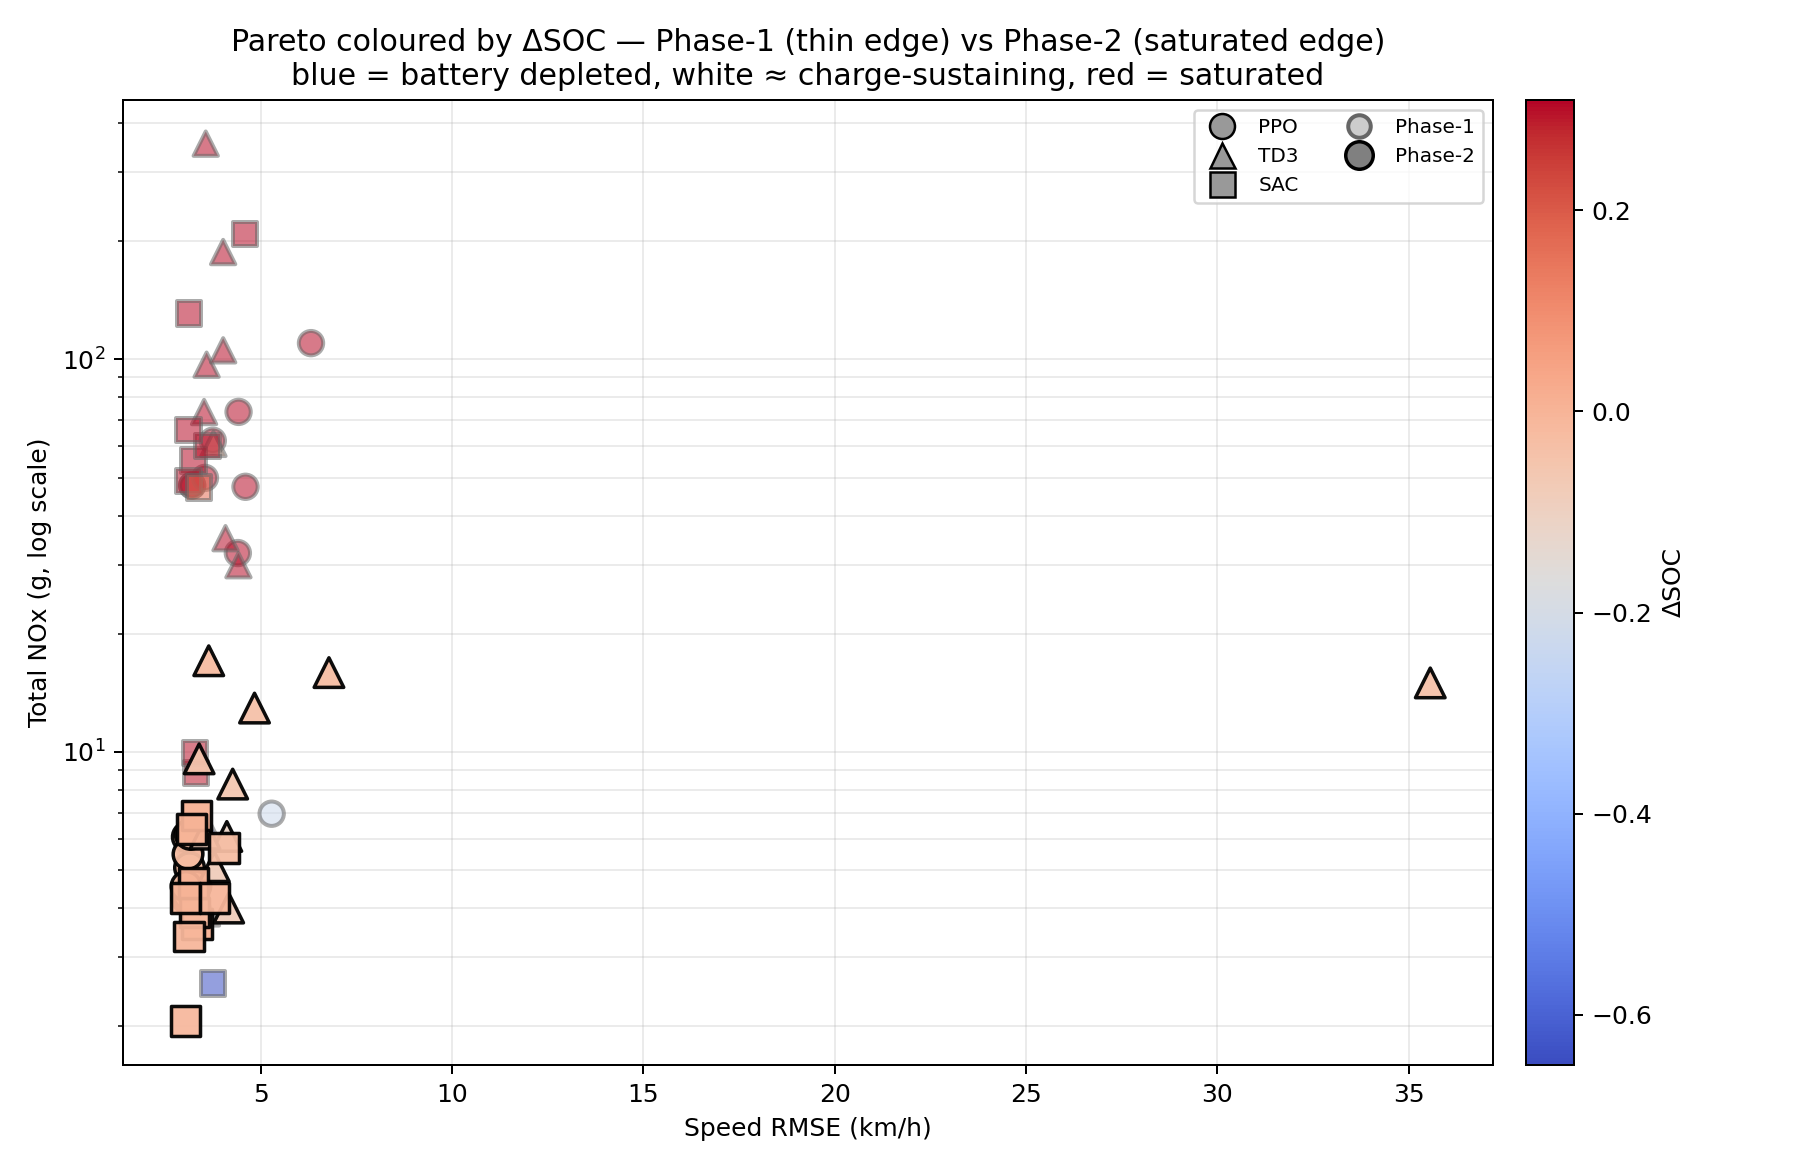
\includegraphics[width=0.7\textwidth]{imgs/analysis_plots/phase2/pareto_overlay_soc.png}
  \caption[Phase-1 vs Phase-2 Pareto picture coloured by charge drift]{Speed-tracking accuracy versus cumulative \ac{NOx} (log axis) for all 30 Phase~1 seeds (thin edge) and 30 Phase~2 seeds (saturated edge). Marker shape encodes the algorithm and fill colour encodes $\Delta$\ac{SOC} (blue = battery depleted, white $\approx$ charge-sustaining, red = saturated). The lone deep-blue low-\ac{NOx} Phase~1 marker is SAC seed~8, isolating the single ``clean'' Phase~1 seed as a battery-depleter.}
  \label{fig:phase2_pareto_overlay}
\end{figure}

\begin{figure}[htbp]
  \centering
  
\includegraphics[width=0.7\textwidth]{imgs/analysis_plots/phase2/parallel_coords.png}
  \caption[Per-seed Phase-2 evaluation metrics in parallel coordinates]{Per-seed Phase~2 evaluation metrics in parallel coordinates. Each polyline is one seed, each axis is normalised independently to its own min--max range (true extrema printed at the axis ends), and colour encodes the algorithm. Contrast with the Phase~1 version in \autoref{fig:phase1_parallel_coords}.}
  \label{fig:phase2_parallel_coords}
\end{figure}

\paragraph{Operating-point shift by reducing \ac{NOx}.}
The emission reduction originates in a shift of the engine operating point toward lower load. Because the tailpipe \ac{NOx} rate rises monotonically with engine torque (\autoref{fig:phase2_nox_rate_vs_torque}; the measured bench data give $\text{Pearson correlation}(\text{torque}, \text{NOx}) = 0.84$), and because the low-\ac{BSFC} efficiency optimum overlaps with the high-load region, lowering \ac{NOx} requires moving \emph{away} from the \ac{BSFC} sweet spot (\autoref{fig:phase1_engine_map_occupancy}). The per-agent engine-load distributions confirm the shift (\autoref{fig:phase2_engine_load_distribution}), and the operating-point overlay on the measured \ac{NOx} map (\autoref{fig:phase2_engine_map_nox}) shows the median operating point dropping out of the brighter high-\ac{NOx} regions into the darker low-\ac{NOx} regions for all three agents.

A notable consequence of the operating-point shift is that fuel consumption falls alongside \ac{NOx} rather than trading off against it (\autoref{tab:phase2_headline}). The Phase~1 policies, lacking any \ac{SOC} penalty, overcharged the battery to its upper clip ($\Delta\text{SOC} \approx +0.30$, \autoref{subsec:results_phase1_summary}). Assuming that overcharge required additional high-load engine operation purely to charge the battery which inflates both fuel and \ac{NOx}. Once the \ac{SOC} term enforces \ac{SOC} maintenance, the engine performs only the tractive work the cycle demands, so both quantities drop together. The same shift is visible on the \ac{BSFC} map (\autoref{fig:phase2_engine_map_bsfc}), read as a slight increase in distance from the efficiency optimum; representing a trade-off, in brake-specific terms, for the large \ac{NOx} reduction.

\begin{figure}[H]
  \centering
  \begin{minipage}[t]{0.49\textwidth}
    \centering
    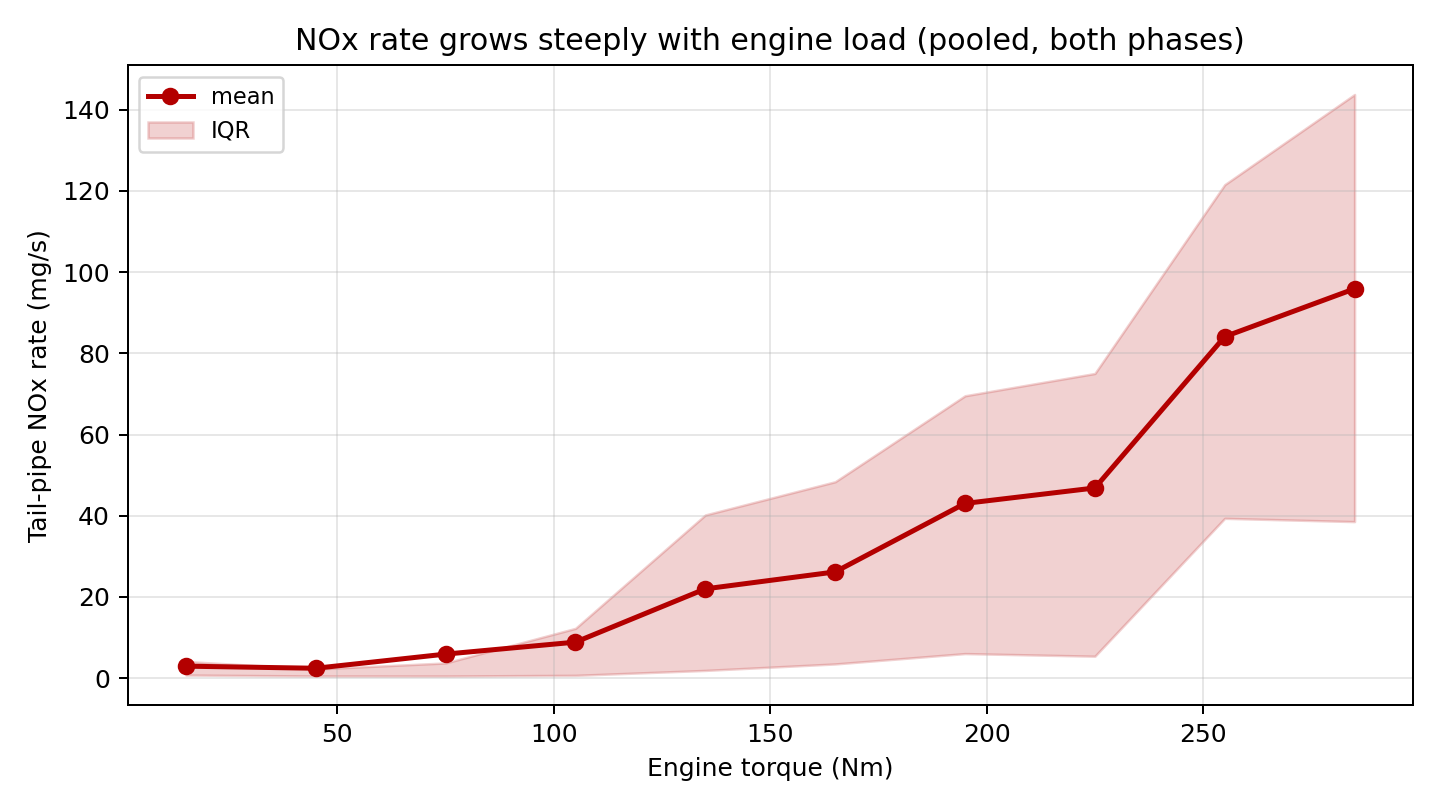
\includegraphics[width=\textwidth]{imgs/analysis_plots/phase2/nox_rate_vs_torque.png}
    \caption[NO\textsubscript{x} rate versus engine torque]{Pooled tail-pipe \ac{NOx} rate as a function of engine torque for both phases and engine-on steps, with the inter-quartile band. The monotonic trend explains why moving to lower engine load reduces \ac{NOx}.}
    \label{fig:phase2_nox_rate_vs_torque}
  \end{minipage}
  \hfill
  \begin{minipage}[t]{0.49\textwidth}
    \centering
    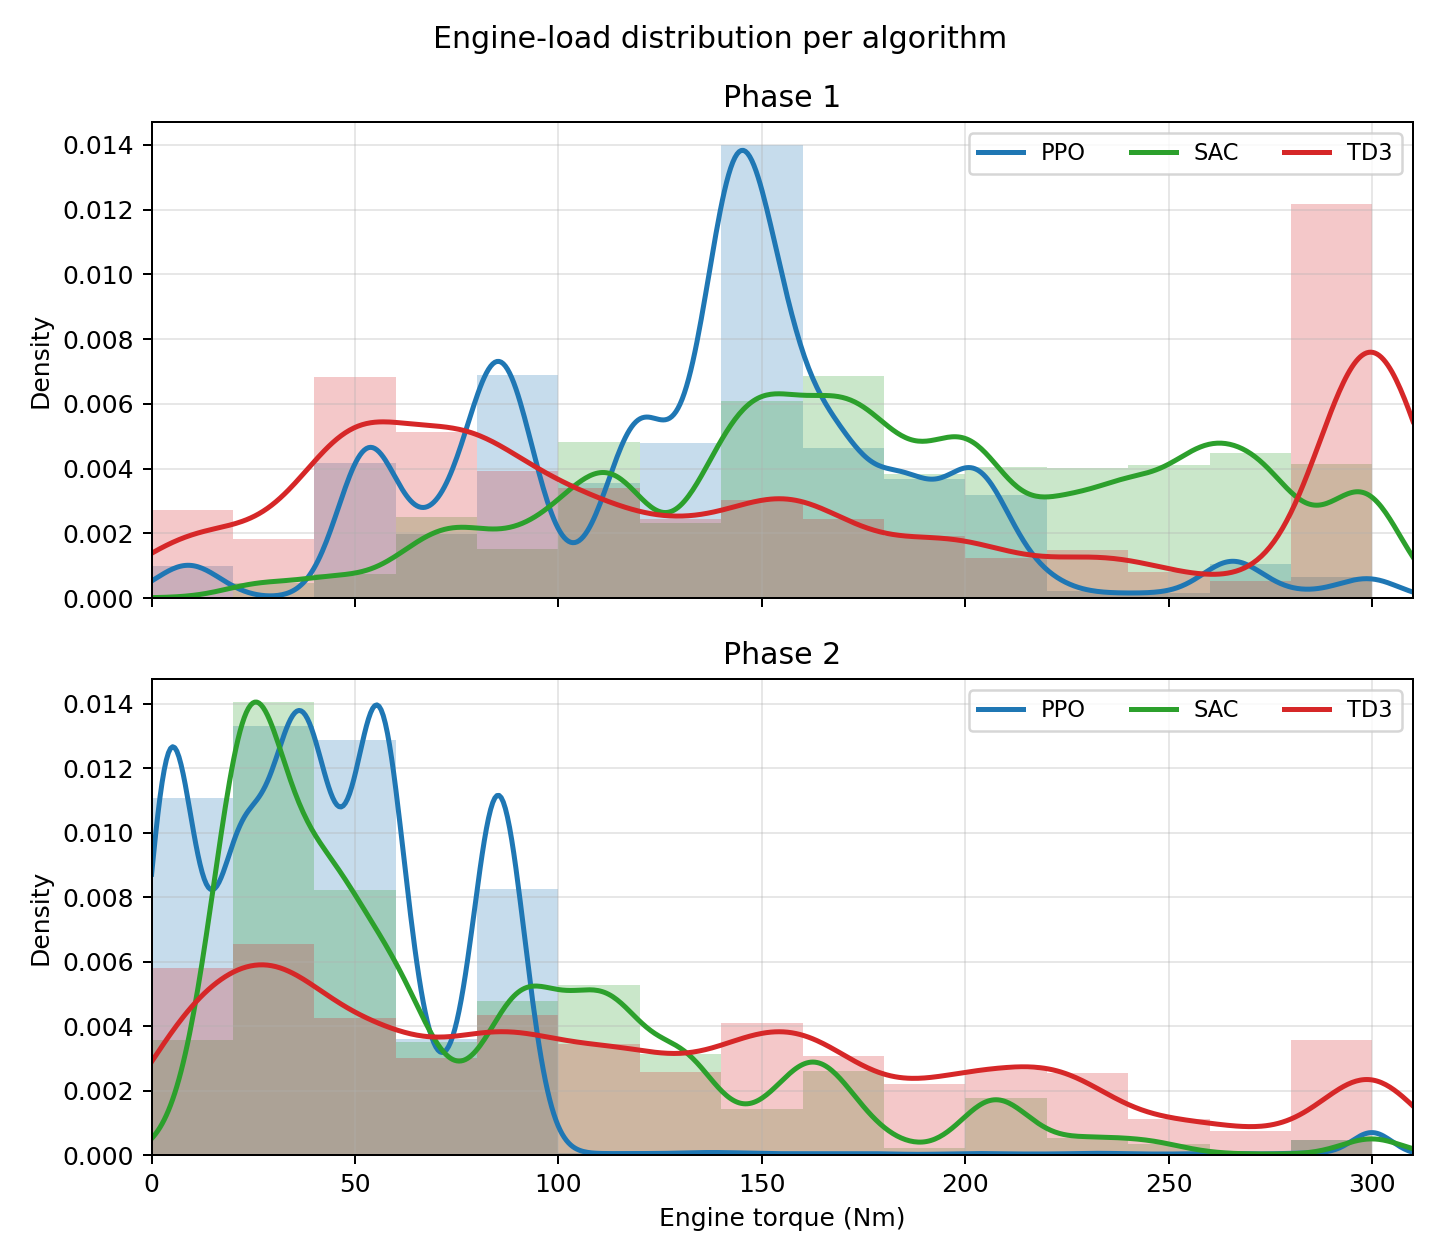
\includegraphics[width=\textwidth]{imgs/analysis_plots/phase2/engine_load_distribution.png}
    \caption[Phase-1/Phase-2 engine-load distributions]{Per-agent engine-torque distributions for Phase~1 (dotted) and Phase~2 (solid). Phase~2 concentrates engine operation at markedly lower load, where \ac{NOx} production is low.}
    \label{fig:phase2_engine_load_distribution}
  \end{minipage}
\end{figure}

\begin{figure}[H]
  \centering
  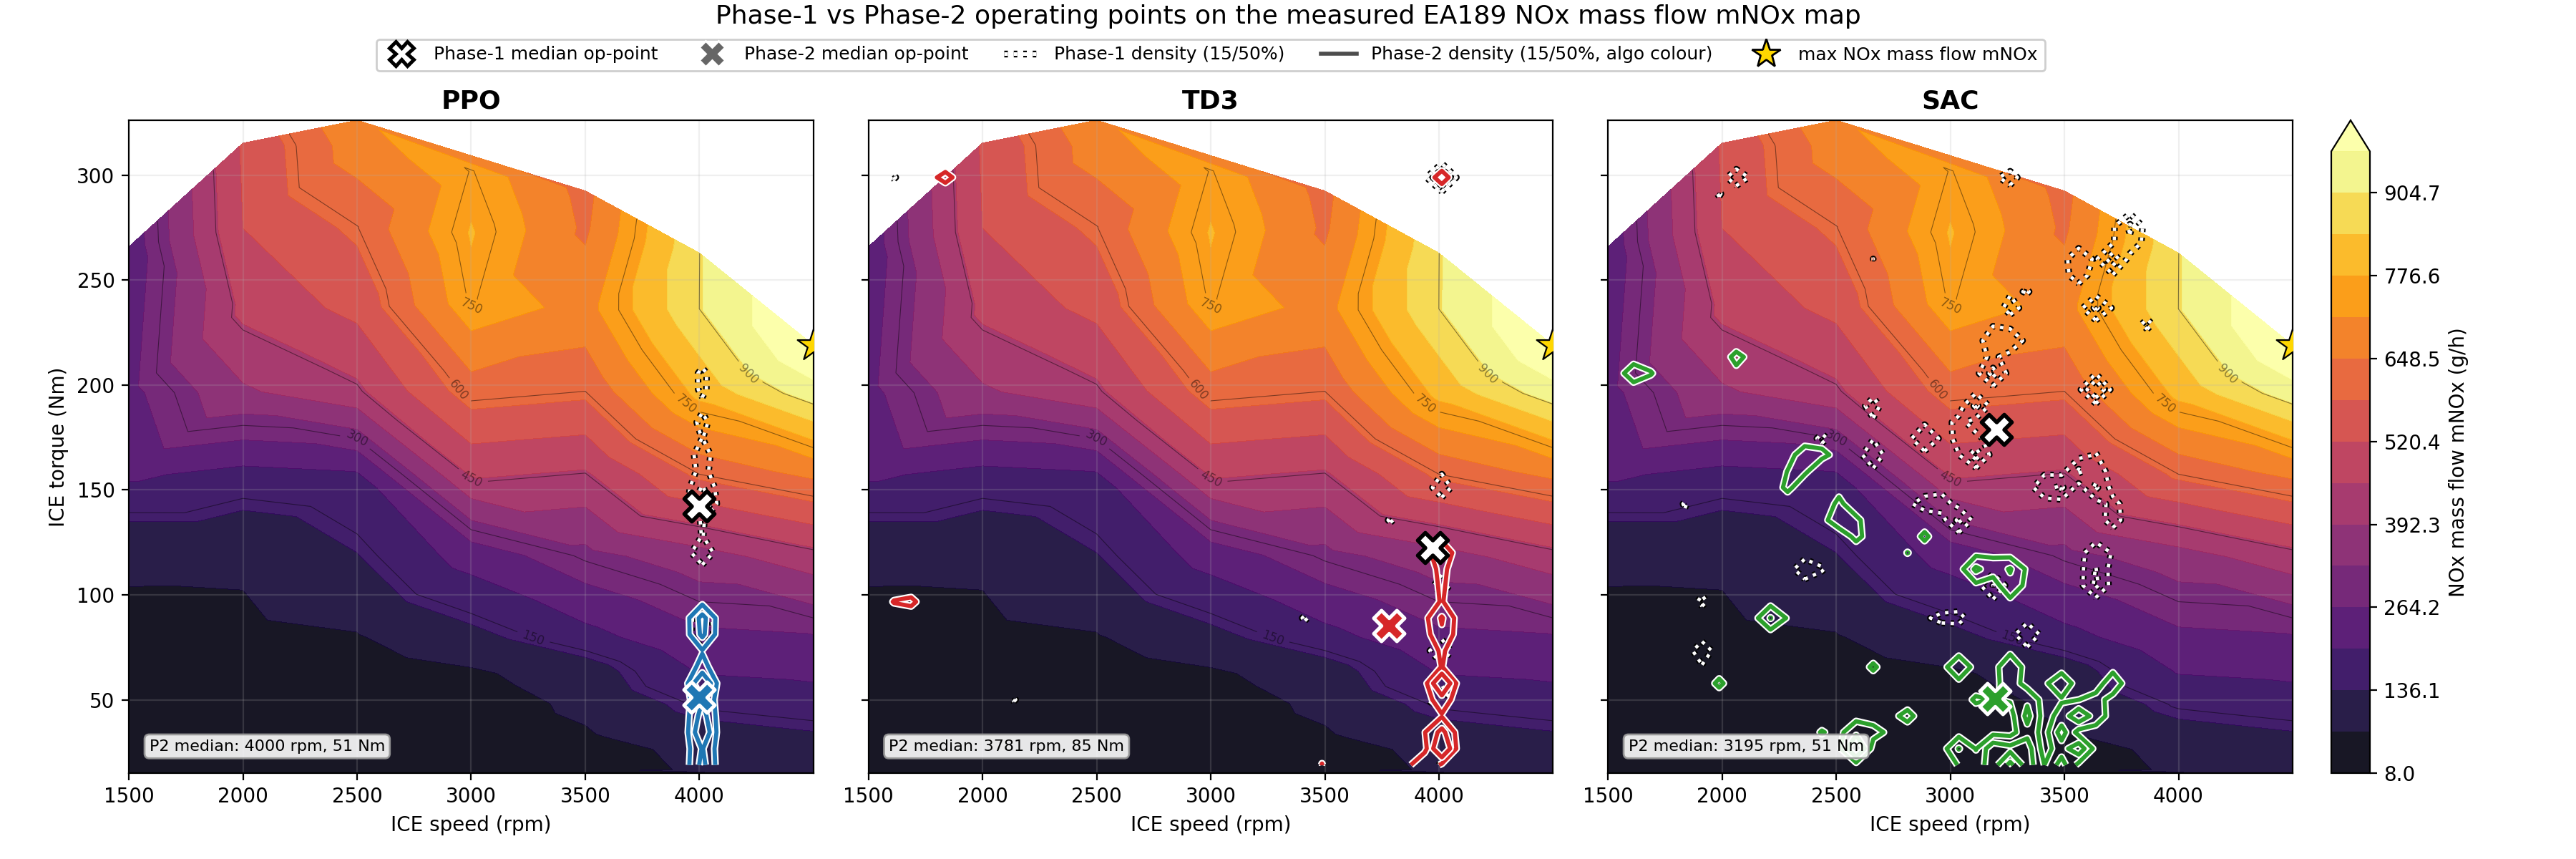
\includegraphics[width=\textwidth]{imgs/analysis_plots/phase2/engine_map_nox_overlay.png}
  \caption[Phase-1 vs Phase-2 operating points over the measured NOx map]{Engine operating points over the measured EA189 \ac{NOx} mass-flow-rate ($\dot m_{\mathrm{NO}_{x},\mathrm{tp}}$) map, interpolated from the same 74 bench points as the \ac{BSFC} map. White markers/contours show the Phase~1 median operating point and density; coloured markers/contours show Phase~2. All three agents move from the bright high-\ac{NOx} band into the dark low-\ac{NOx} band.}
  \label{fig:phase2_engine_map_nox}
\end{figure}

\begin{figure}[H]
  \centering
  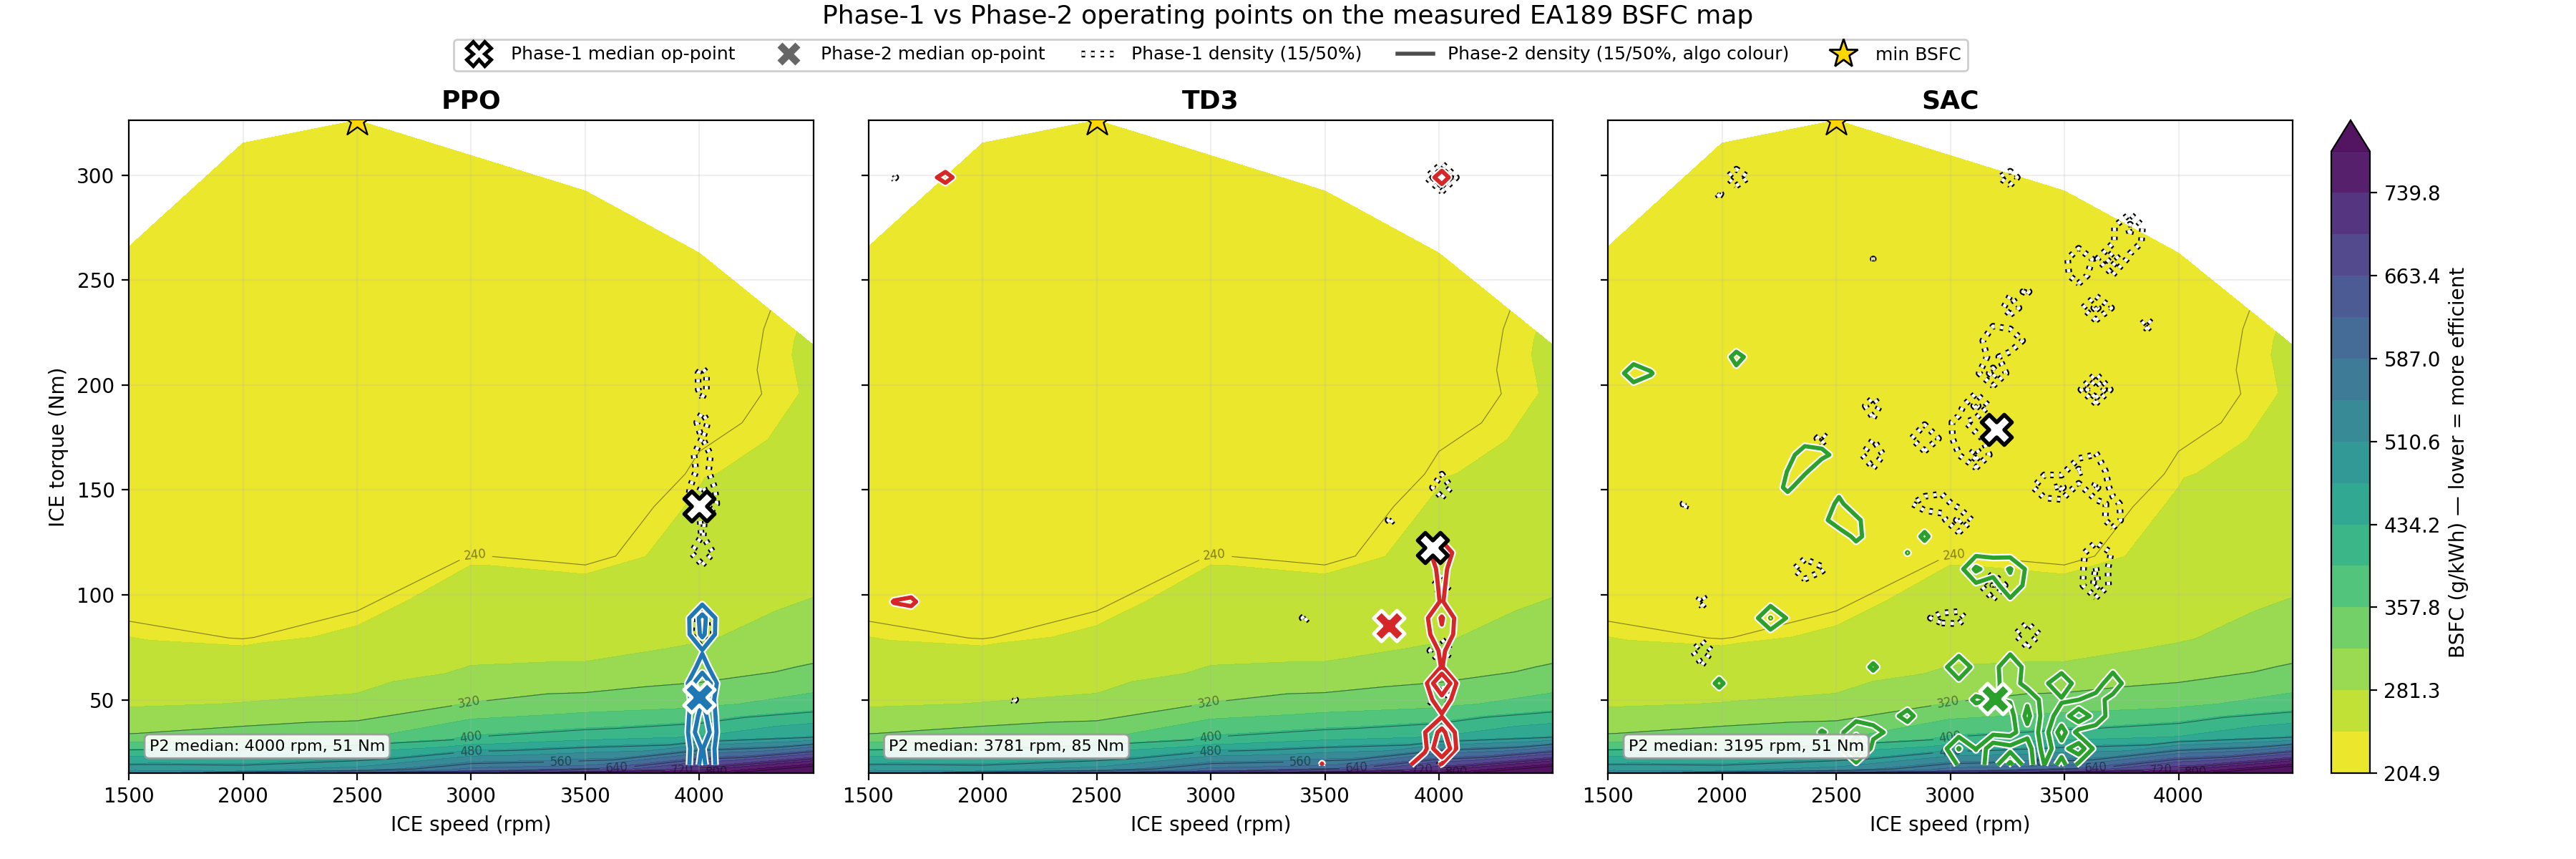
\includegraphics[width=\textwidth]{imgs/analysis_plots/phase2/engine_map_bsfc_overlay.png}
  \caption[Phase-1 vs Phase-2 operating points over the measured BSFC map]{Engine operating points over the measured EA189 \ac{BSFC} map. White markers/contours show Phase~1, coloured markers/contours show Phase~2. The Phase~2 policies move to lower load, slightly away from the most efficient measured point (gold star), trading a small amount of brake-specific efficiency for the large \ac{NOx} reduction shown in \autoref{fig:phase2_engine_map_nox}.}
  \label{fig:phase2_engine_map_bsfc}
\end{figure}

\paragraph{Algorithm recommendation.}
Where Phase~1 SAC had the lowest speed tracking variance, Phase~2 highlights that \textbf{PPO is the most accurate candidate}; it transfers with the smallest tracking penalty and the lowest seed-to-seed variance. Meanwhile \textbf{SAC is the strongest emission performer} and the natural choice when minimum \ac{NOx} is the priority. \textbf{TD3 is excluded} as a candidate due to the training instability documented in \autoref{subsec:results_phase2_td3}. The validation that motivated Phase~2 is met for the two stable agents: emissions are reduced and the battery charge is maintained, without a meaningful loss of speed-tracking quality. The remaining gap to the Euro~6 limit, the staircase-versus-\ac{WLTC} caveat, and the TD3 instability are taken up in \autoref{chap:discussion}.

\section{Generalisation Evaluation on the WLTC}
\label{sec:wltc-comparison}

The preceding analysis was specific to the synthetic staircase speed trajectory used for training and evaluation. To assess whether the resulting policies generalise to a more realistic driving mission, the Phase~2 PPO and SAC agents are evaluated zero-shot on the standardised \ac{WLTC} and compared with a rule-based controller. This comparison is motivated by current industry practice, which still relies heavily on rule-based solutions because of their interpretability and reliability, as discussed in \autoref{sec:problem_description}. Frey et al. \cite{frey_data-based_2025} provide the reference benchmark used here by developing such a rule-based strategy and evaluating it on the \ac{WLTC}.

All ten PPO and SAC seeds are evaluated without retraining; TD3 is omitted because the Phase~2 results showed insufficient training stability. For a fair, charge-sustaining comparison, the \ac{RL} agents, which start and return to $\mathrm{SOC}\approx0.70$, are matched against the rule-based \emph{isoSOC} run ($\mathrm{SOC}\approx0.56$); both settings are charge-neutral over the cycle.

\subsection{Population-Level Picture (10 seeds)}

Table~\ref{tab:wltc-mean} aggregates the ten seeds per algorithm as mean\,$\pm$\,standard deviation. Both RL algorithms track the WLTC target more tightly than the rule-based controller (PPO RMSE $0.81$ vs $2.29$\,km/h),
demonstrating that the learned policies transfer zero-shot to an unseen, realistic cycle. However, they do so at higher tailpipe-\ac{NOx} and fuel cost: the phase-2 reward places no weight on fuel ($w_\text{fuel}=0$), so the agents keep the engine running almost continuously (PPO $0\%$ idle-off) and burn $1.6$--$2.2\times$ the rule-based fuel while emitting $\sim$17\% more \ac{NOx}.

\begin{table}[H]
  \centering
  \small
  \begin{tabular}{lrrrrrr}
    \toprule
    Controller & NOx & Fuel & RMSE & MAE & $\Delta$SOC & Eng.\ off \\
    & (mg/km) & (g) & (km/h) & (km/h) & & (\%) \\
    \midrule
    PPO (10)   & $172\pm13$ & $3060\pm52$  & $0.81\pm0.18$ & $0.61\pm0.16$ & $-0.027\pm0.006$ & $0\pm0$  \\
    SAC (10)   & $173\pm41$ & $2223\pm285$ & $1.64\pm0.68$ & $1.30\pm0.73$ & $+0.004\pm0.013$ & $13\pm24$ \\
    Rule-based & $147$      & $1376$       & $2.29$        & $1.73$        & $+0.003$         & $16$ \\
    \bottomrule
  \end{tabular}
  \caption[WLTC 10-seed mean comparison]{WLTC, 10-seed mean\,$\pm$\,std vs.\ the rule-based controller.}
  \label{tab:wltc-mean}
\end{table}

These averages must be read with care. The standard deviations are partly large and, more fundamentally, the ten seeds still inherit variations in the control policy and are not noisy realisations of one controller. Accordingly, averaging distinct strategies should be avoided since it describes no controller that actually exists and obscures the best achievable, individual behaviour. For the purpose of further development a \emph{single} seed must therefore be selected and carried forward, rather than the seed-averaged number.

\begin{figure}[htbp]
  \centering
  \centering
  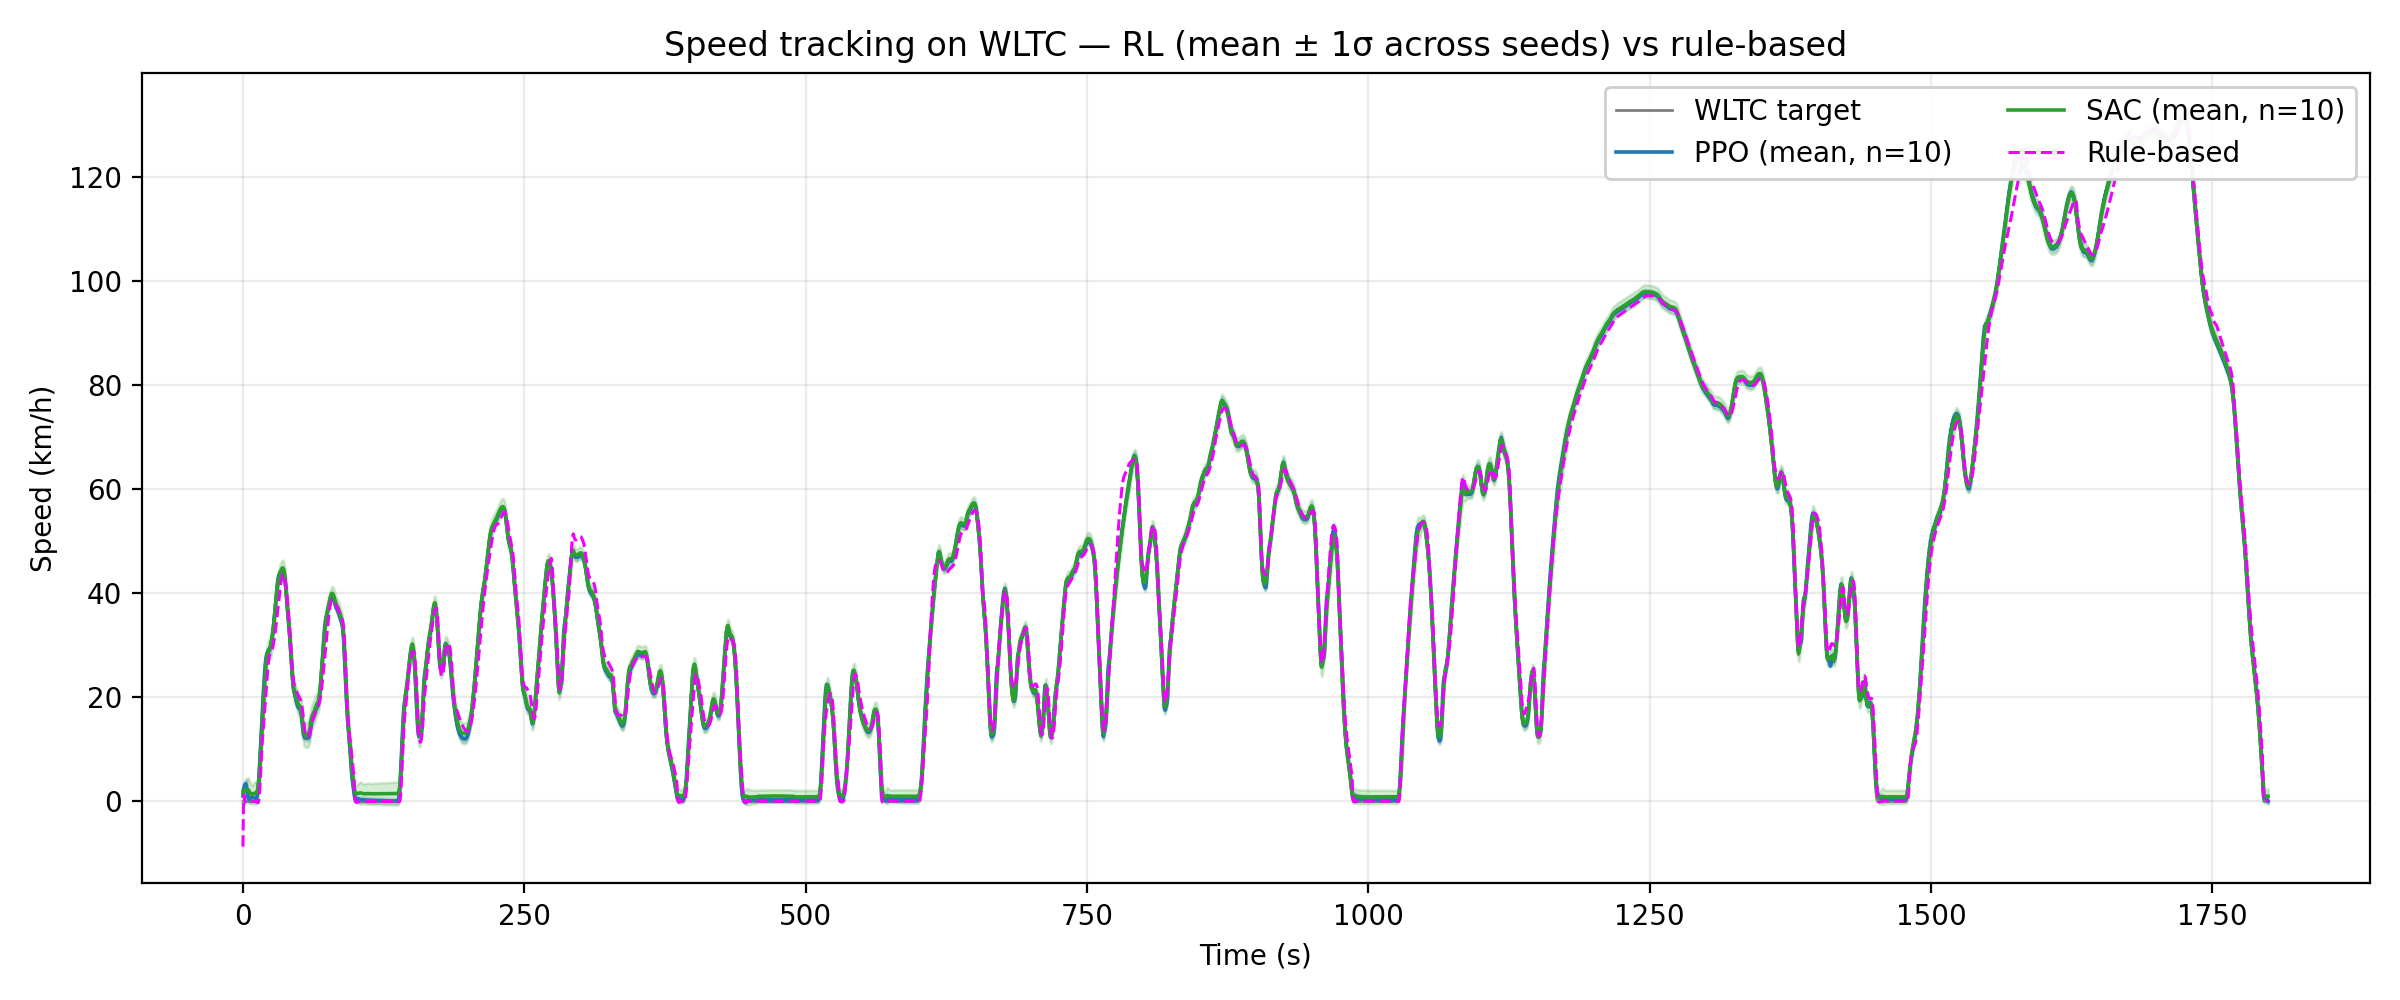
\includegraphics[width=0.85\textwidth]{imgs/plots/wltc_comparison/speed_tracking_wltc.png}
  \caption[WLTC speed-tracking comparison]{Speed tracking on the WLTC. RL mean\,$\pm$\,$1\sigma$ across $10$ seeds per algorithm vs. the rule-based controller. Both RL algorithms follow the target trace closely across the full cycle.}
  \label{fig:wltc-tracking}
\end{figure}

\begin{figure}[htbp]
  \centering
  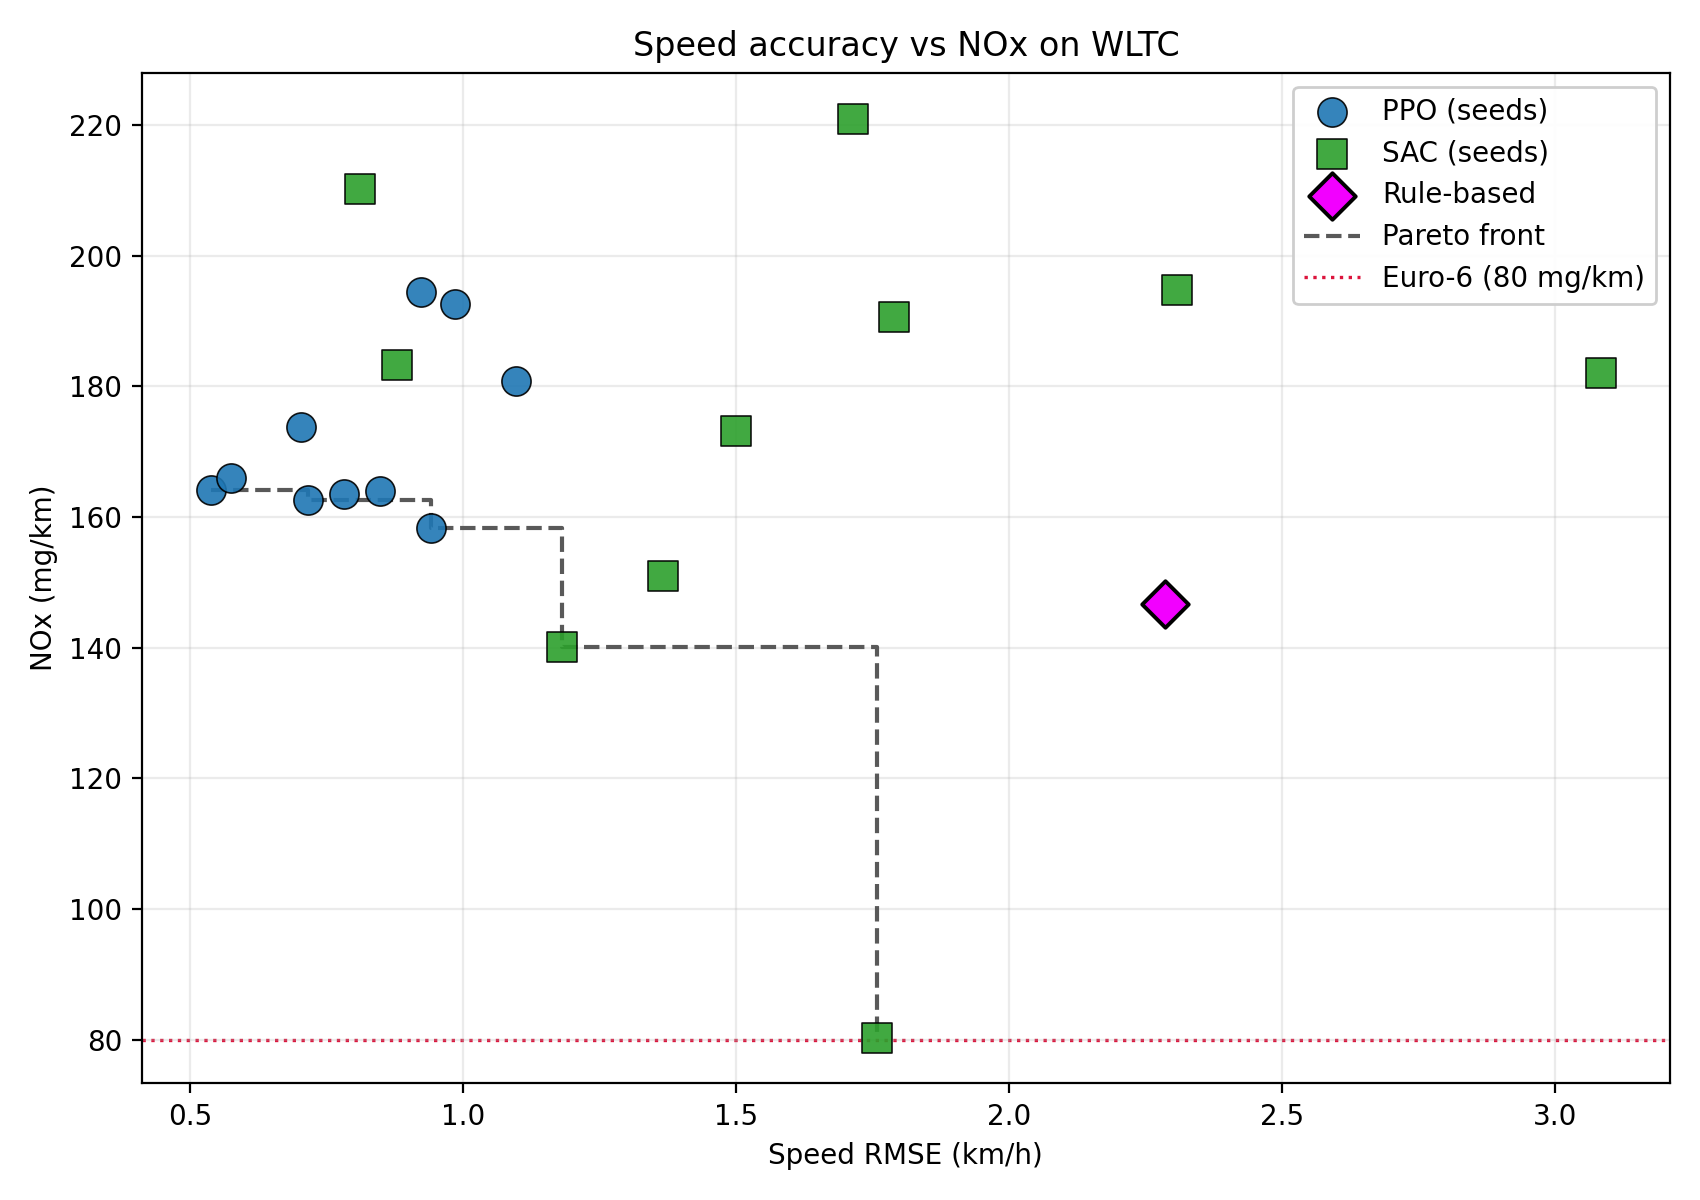
\includegraphics[width=0.7\textwidth]{imgs/plots/wltc_comparison/pareto_wltc.png}
  \caption[WLTC speed--NOx Pareto comparison]{Speed RMSE vs. tailpipe NOx on the WLTC, one marker per seed. The single SAC seed on the Euro-6 line (80\,mg/km) is seed~7, the best candidate.}
  \label{fig:wltc-pareto}
\end{figure}

\begin{figure}[htbp]
  \centering
  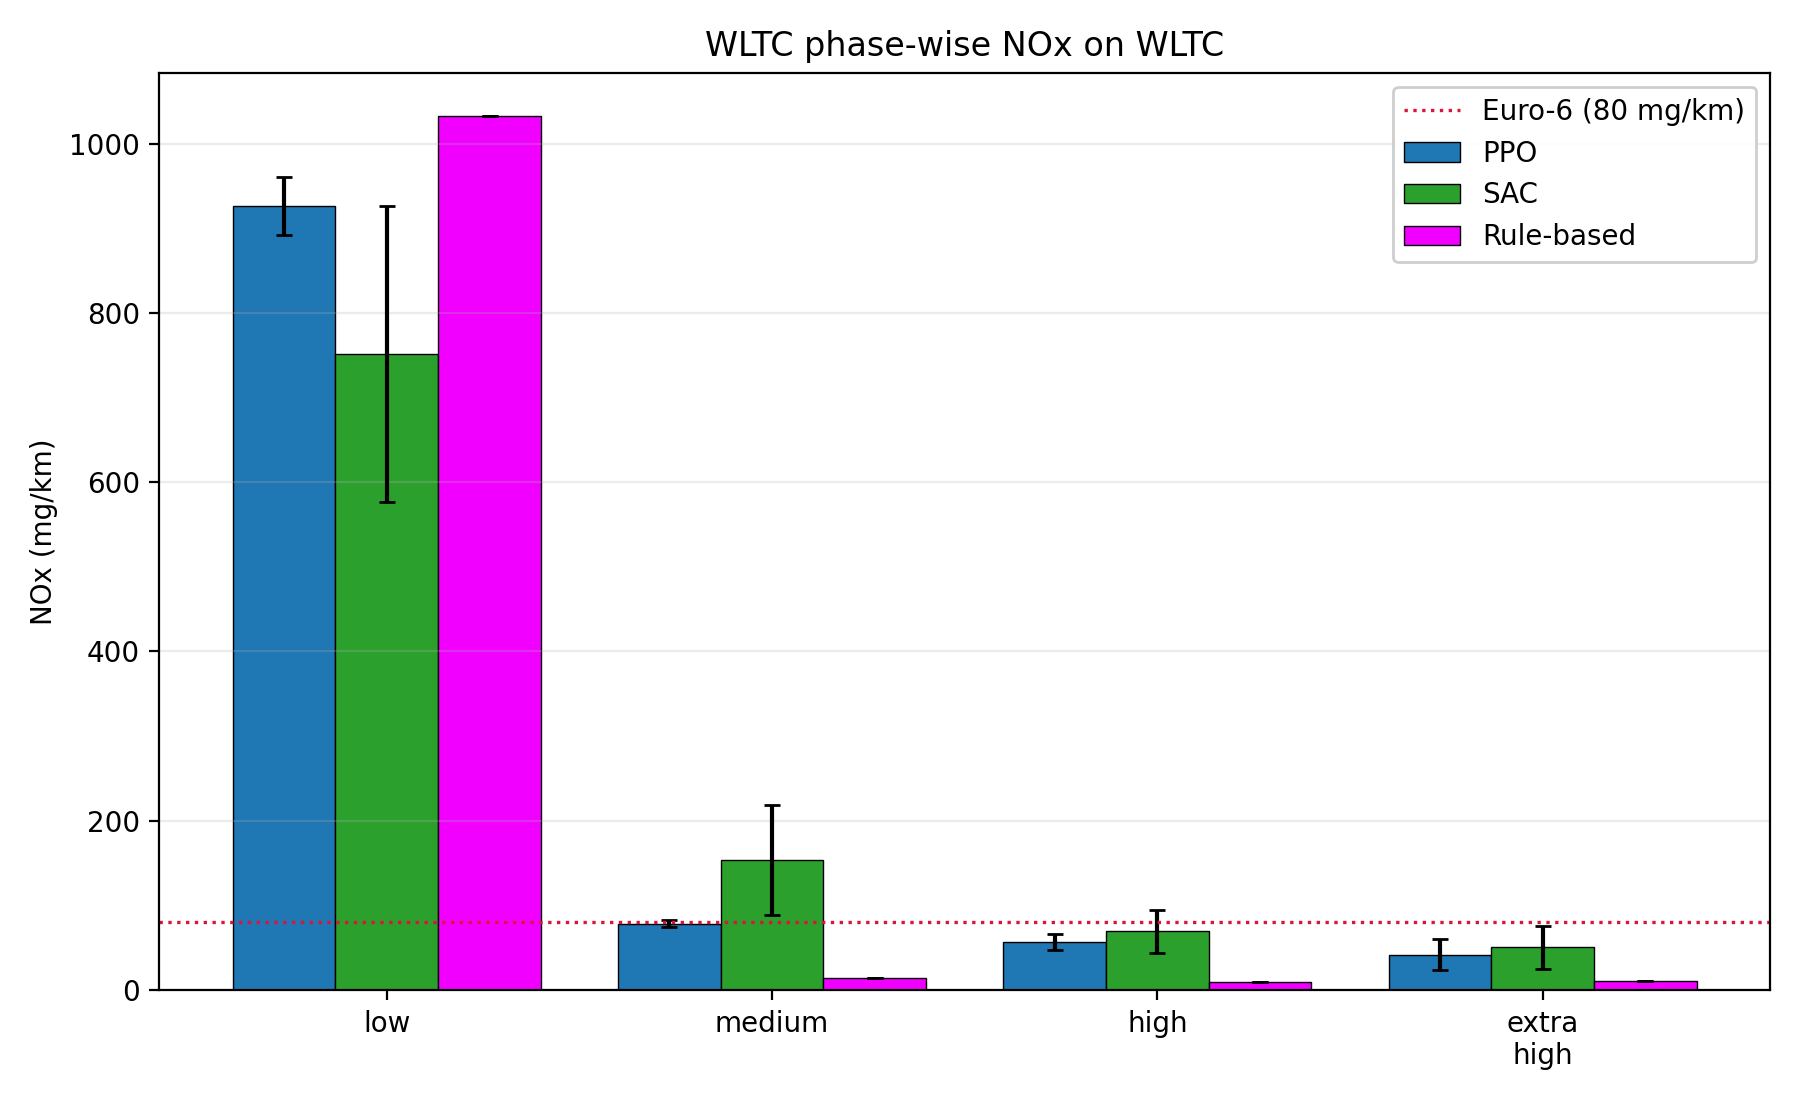
\includegraphics[width=0.65\textwidth]{imgs/plots/wltc_comparison/phase_nox_wltc.png}
  \caption[WLTC phase-wise NOx comparison]{WLTC phase-wise tailpipe NOx (mg/km), per-algorithm seed mean vs. the rule-based controller, against the Euro-6 80\,mg/km limit.}
  \label{fig:wltc-phasenox}
\end{figure}

\subsection{Best-Seed Comparison}

Selecting one seed per algorithm with the composite score used throughout phase~2 yields \textbf{PPO seed~2} and \textbf{SAC seed~7}
(Table~\ref{tab:wltc-best}).

\begin{table}[H]
  \centering
  \small
  \begin{tabular}{lrrrrrr}
    \toprule
    Controller & NOx & Fuel & RMSE & MAE & $\Delta$SOC & Eng.\ off \\
    & (mg/km) & (g) & (km/h) & (km/h) & & (\%) \\
    \midrule
    PPO seed~2 & $158$ & $3087$ & $0.94$ & $0.75$ & $-0.024$ & $0$  \\
    SAC seed~7 & $80$  & $1730$ & $1.76$ & $1.09$ & $+0.010$ & $57$ \\
    Rule-based & $147$ & $1376$ & $2.29$ & $1.73$ & $+0.003$ & $16$ \\
    \bottomrule
  \end{tabular}
  \caption[WLTC best-seed comparison]{WLTC, best seed per algorithm vs. the rule-based controller.}
  \label{tab:wltc-best}
\end{table}

The selected seeds reverse the unfavourable population-level reading. \emph{SAC seed~7 outperforms the rule-based controller on both \ac{NOx} and speed tracking}: it reduces tailpipe \ac{NOx} by $\sim$45\% (80\,mg/km vs.\ 147\,mg/km, i.e.\ to the Euro~6 limit), tracks the target more accurately (RMSE $1.76$ vs.\ $2.29$\,km/h), and remains charge-sustaining ($\Delta\text{SOC}=+0.010$). This performance is achieved by switching the engine off for $57\%$ of the cycle --- far more than the rule-based controller's $16\%$ --- at the cost of $\sim$26\% higher fuel consumption. The \ac{EM2} command spans the full feasible range, supporting \ac{SOC} sustainment and vehicle propulsion, but remains concentrated around $50$. Compared with the staircase cycle, braking is used more frequently, which is consistent with the greater variability of the \ac{WLTC} speed trajectory. The \ac{ICE} speed distribution has a much larger mass at 0\,rpm due to the engine-off phases, while fuel injection shows engine start-up spikes followed by rapid cutback to approximately half of the spike value. The action summary and the resulting velocity, \ac{SOC}, and tailpipe \ac{NOx} emissions are depicted in \autoref{fig:wltc_sac_action_summary} and \autoref{fig:wltc_sac_seed7_evaluation_results}, respectively.
PPO seed~2, by contrast, attains the best speed tracking of all controllers ($0.94$\,km/h) but does not beat the rule-based baseline on \ac{NOx} and retains the always-on, high-fuel behaviour. \textbf{SAC seed~7 is therefore the selected candidate for continued development.}

% --------------------------------------------------------------------- %

\begin{figure}[H]
  \centering
  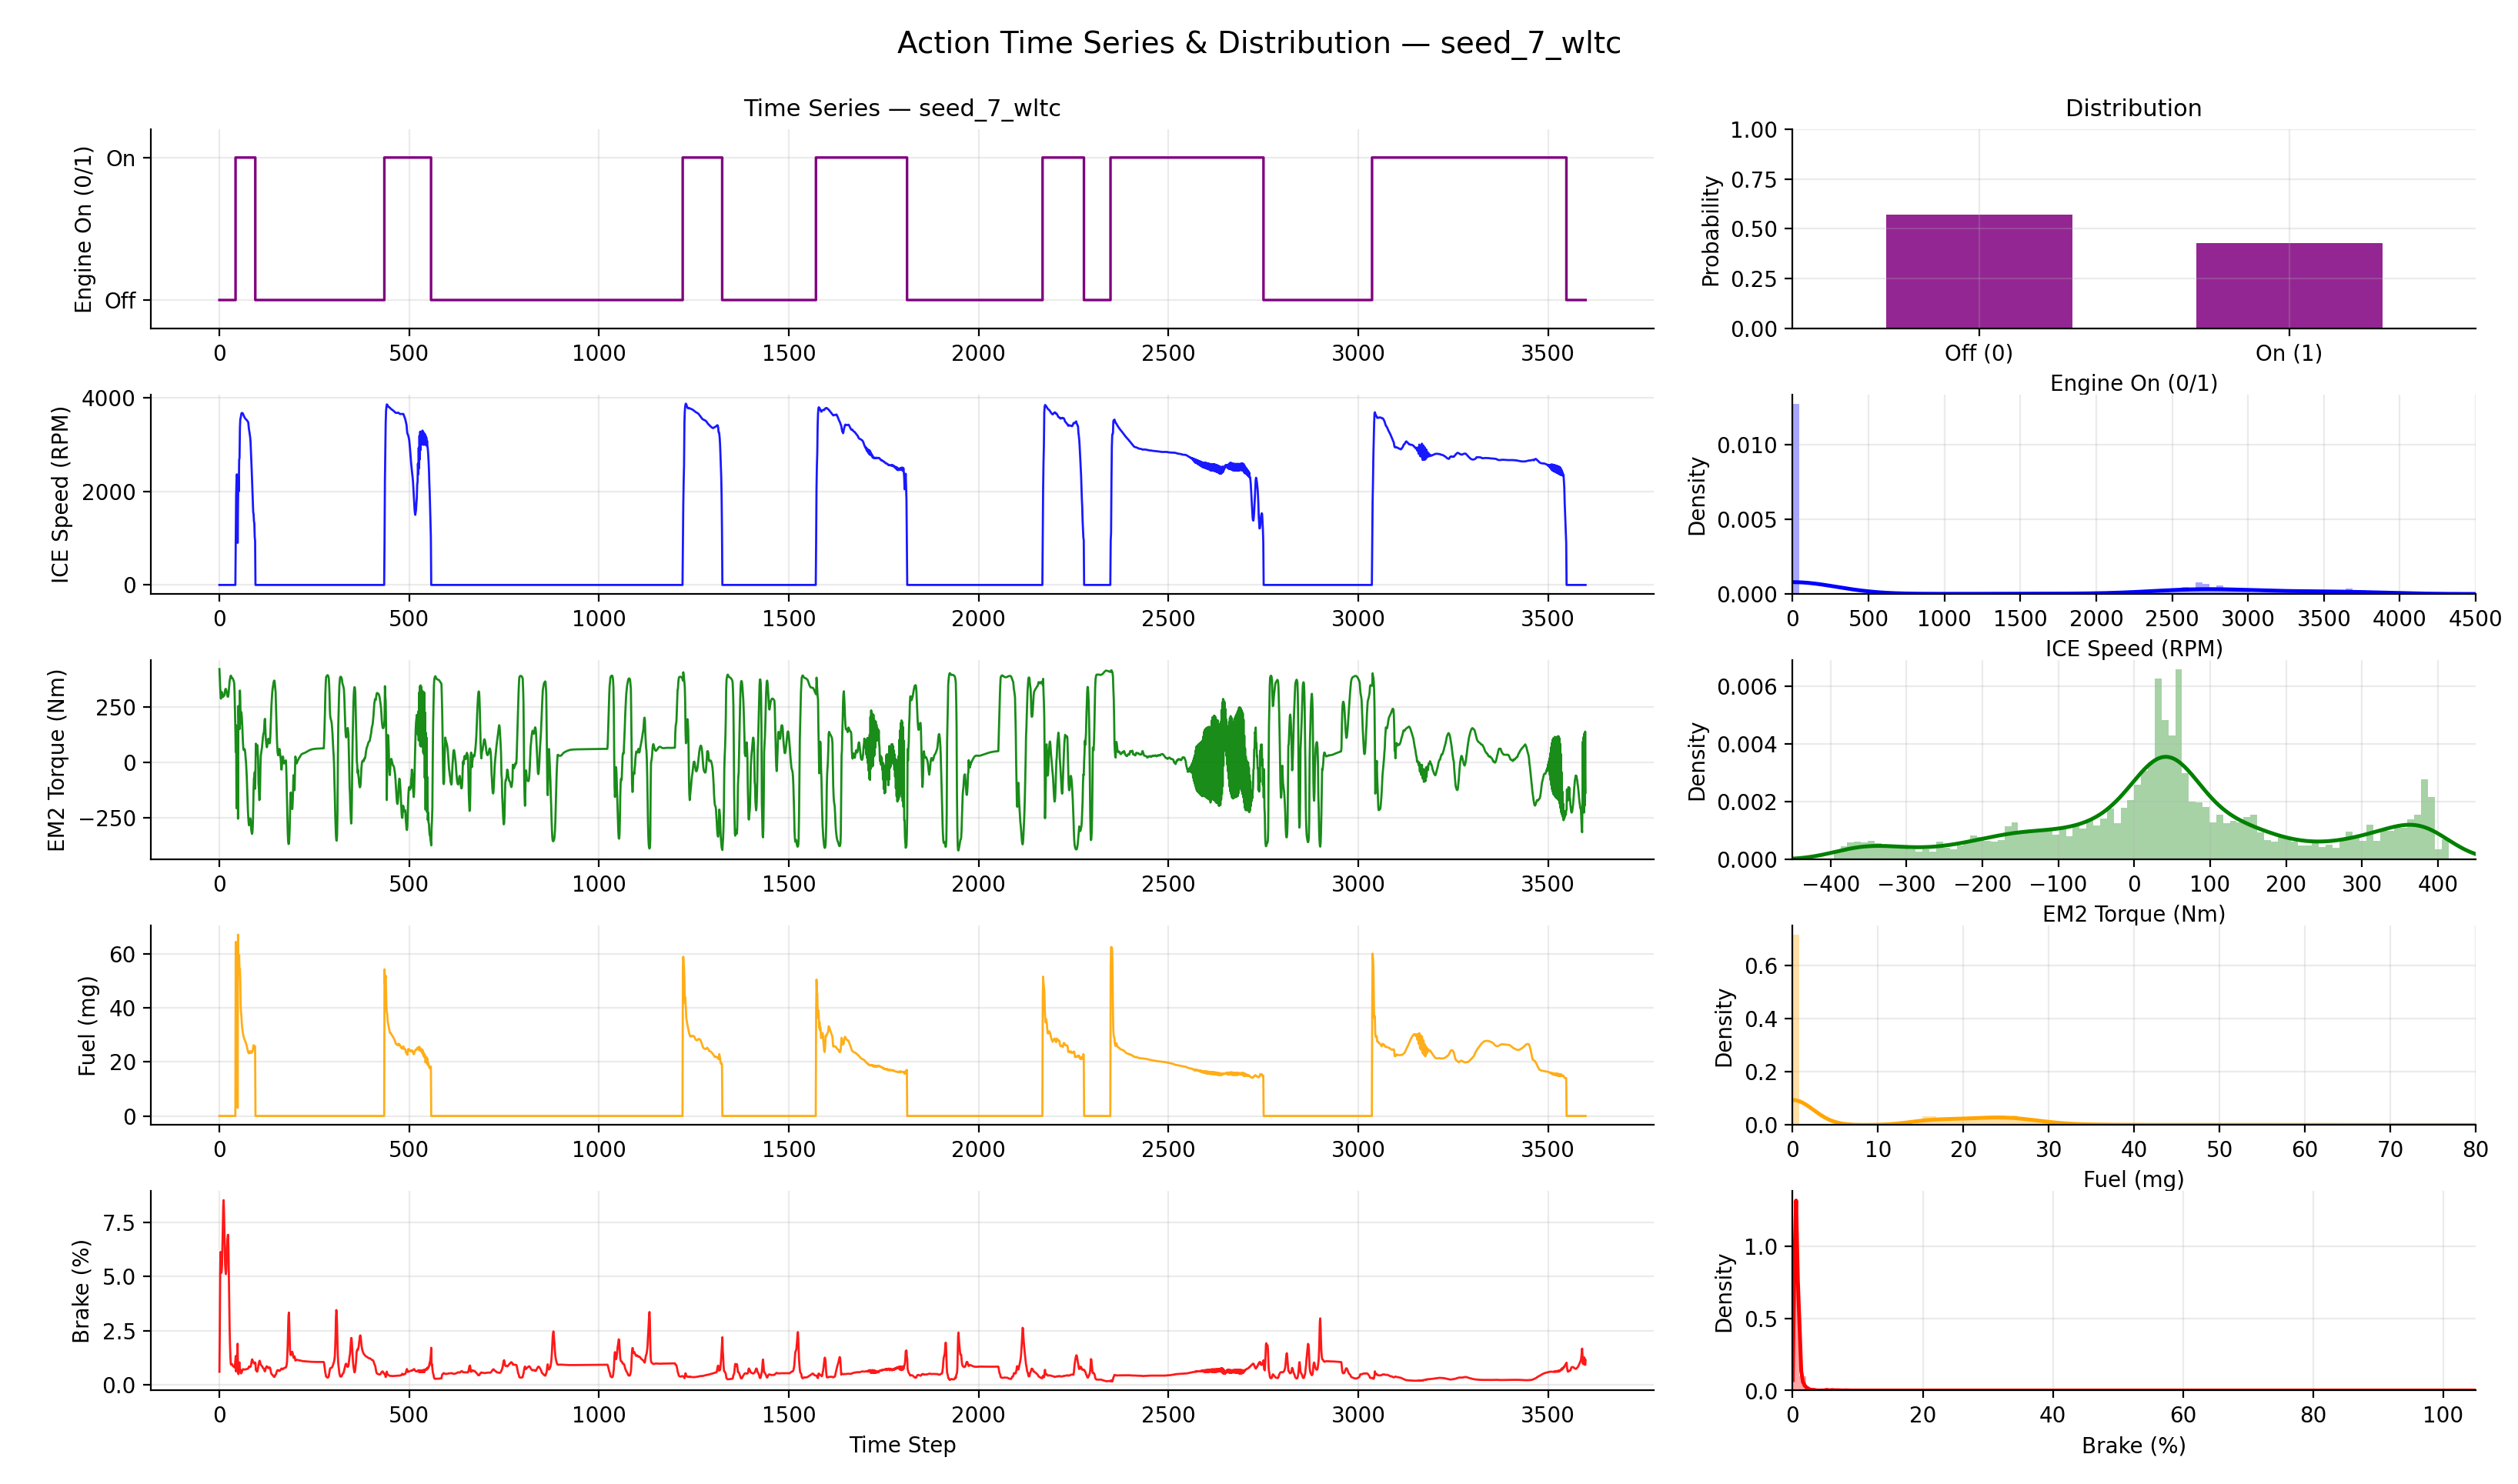
\includegraphics[width=\textwidth]{imgs/plots/wltc_comparison/seed_7_wltc_action_summary.png}
  \caption[Best SAC seed action summary on WLTC]{Action summary for the best SAC checkpoint, seed~7, on the WLTC. The left panels show the SAC agent's actions during the WLTC; the right panels show the corresponding densities.}
  \label{fig:wltc_sac_action_summary}
\end{figure}

\begin{figure}[H]
  \centering
  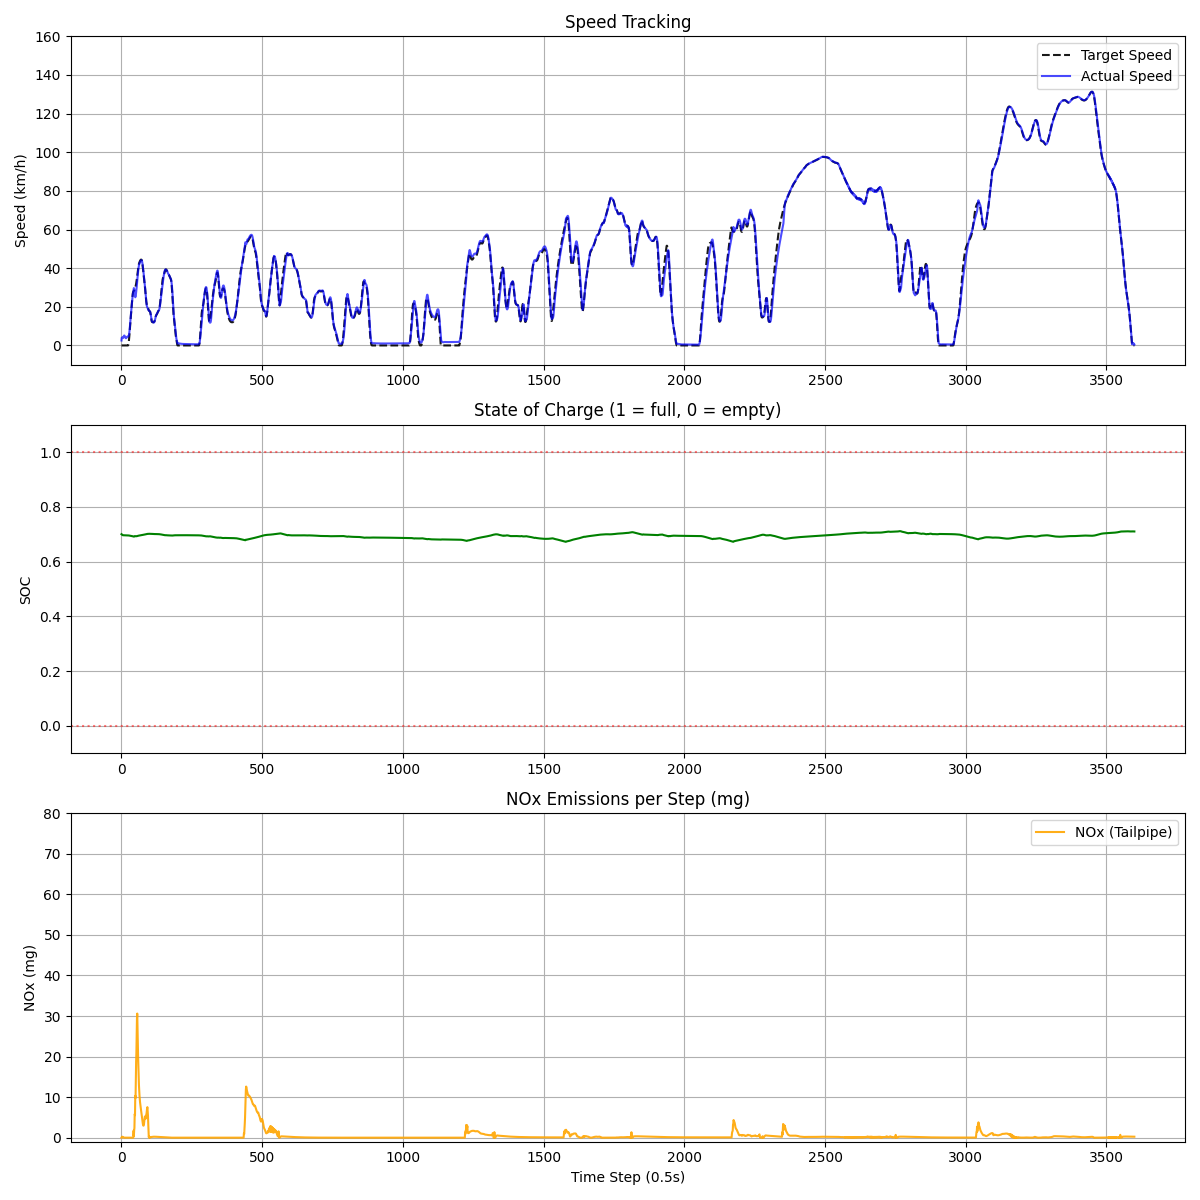
\includegraphics[width=0.55\textwidth]{imgs/plots/wltc_comparison/seed_7_wltc_evaluation_results.png}
  \caption[Best SAC seed evaluation results on WLTC]{Evaluation results for the best SAC checkpoint, seed~7, on the WLTC. The panels show speed tracking, the \ac{SOC} trajectory, and tailpipe \ac{NOx} emissions over the evaluation cycle.}
  \label{fig:wltc_sac_seed7_evaluation_results}
\end{figure}
